
% \setchapterpreamble[ur]{%
% \dictum[G.~Box~\cite{box1987empirical}]{%
% All models are wrong, but some are useful.}%
% \vspace*{2cm}}



%%%%%%%%%%%%%%%%%%%%%%%%%%%%%%%%%%%%%%%%%%%%%%%%%%%%%%%%%%%%
\chapter{Higgs effective theory at its limits}
\label{chapter:validity}
%%%%%%%%%%%%%%%%%%%%%%%%%%%%%%%%%%%%%%%%%%%%%%%%%%%%%%%%%%%%

\firstword{A}{ suitable effective field theory} can universally
describe all signatures expected from new physics as long as the new
physics scale $\Lambda$ is much larger than the experimental momentum
transfer. However, the limited precision of the LHC means that Higgs
measurements are often only sensitive to models characterised by mass
scales just above the electroweak scale. In this chapter we discuss if
and when the EFT approach is nevertheless useful, and how its validity
can be improved.

In \autoref{sec:validity_introduction} we estimate the new physics
scales probed by LHC Higgs measurements and formulate our strategy to
test the dimension-six approach. The validity of the effective
approach at the LHC depends on details of the matching procedure,
which we discuss in
\autoref{sec:validity_matching}. \autoref{sec:validity_full_vs_effective}
contains the bulk of our results: the comparison of full models to
their EFT approximations for a variety of scenarios. We go into more
detail and analyse some practical questions in
\autoref{sec:validity_practical_questions}, and present our
conclusions in \autoref{sec:validity_conclusions}.

Most of the work presented in this chapter was previously published in
Reference~\cite{Brehmer:2015rna}, while the content of
\autoref{sec:validity_practical_questions} was published in
Reference~\cite{Biekotter:2016ecg}. A part of the content of this
chapter was also included in
Reference~\cite{deFlorian:2016spz}. Nearly all of the results and most
of their presentation in this chapter\,---\,including most plots and
tables as well as a significant part of the text\,---\,are identical
to that in these three publications.



%%%%%%%%%%%%%%%%%%%%%%%%%%%%%%%%%%%%%%%%%%%%%%%%%%%%%%%%%%%%
\section{Introduction}
\label{sec:validity_introduction}
%%%%%%%%%%%%%%%%%%%%%%%%%%%%%%%%%%%%%%%%%%%%%%%%%%%%%%%%%%%%

%%%%%%%%%%%%%%%%%%%%%%%%%%%%%%%%%%%%%%%%%%%%%%%%%%%%%%%%%%%%
% \subsection{Energy scales in Higgs measurements}
% \label{sec:validity_introduction_scales}
%%%%%%%%%%%%%%%%%%%%%%%%%%%%%%%%%%%%%%%%%%%%%%%%%%%%%%%%%%%%

There is no doubt that effective field theories work extraordinarily
well as long as there is a scale hierarchy between the experimentally
probed energy and the new physics scale, $E \ll \Lambda$. On the other
hand, one expects the EFT expansion to break down at $E \geq \Lambda$,
where an infinite number of operators contribute at the same size and
the effective model is neither predictive nor renormalisable. The
validity of the EFT in the intermediate region, $E \lesssim \Lambda$,
is less obvious and will depend on the specific underlying model as
well as on the observable studied.

In which of these categories do the LHC Higgs measurements fall?
There is no immediately obvious answer, since Higgs production does
not probe only a single experimental energy scale. While the momentum
transfer is bounded from below by the Higgs mass $m_h$, selection criteria
necessary to separate a signal from the QCD backgrounds often require
a higher momentum transfer $E > m_h$. More importantly, most of the
information on operators with derivatives comes from high-energy
tails, as demonstrated in \autoref{sec:foundations_heft_pheno}. During
Run~1, significant event numbers have been recorded approximately
within the range~\cite{Corbett:2015ksa}
%
\begin{equation}
  m_h \leq E \lesssim \ord{400~\gev} \,,
  \label{eq:validity_experimental_energy_scale}
\end{equation}
%
depending on the process, observable, collected amount of data, and
analysis methods.

This has to be compared to the new physics scale $\Lambda$ that LHC
Higgs measurements are able to probe. Assuming a $10\%$ precision on
total Higgs rate measurements and no loop suppression of new physics
effects, such a signature lies within the experimental reach of the
LHC if
%
\begin{equation}
  \left| \frac{\sigma \times \text{BR}}{\left( \sigma \times \text{BR} \right)_\text{SM}} - 1 \right|
  \approx \frac{g^2 m_h^2}{\Lambda^2}
  \gtrsim 10\%
  \qquad \Leftrightarrow \qquad 
  \Lambda \lesssim \frac{g \, m_h}{\sqrt{10\%} } \, \approx g \cdot 400~\gev \,.
  \label{eq:validity_probed_scale_estimation}
\end{equation}
%
where $g$ are the typical couplings of the underlying theory and
$\sigma \times \BR$ the Higgs production cross section times branching
ratio.
%
% For loop-induced new physics effects, the corresponding loop
% suppression factor pulls $\Lambda$ to even lower values,
% %
% \begin{equation}
%   \left| \frac{\sigma \times \text{BR}}{\left( \sigma \times \text{BR} \right)_\text{SM}} - 1 \right|
%   = \frac{ g^2 m_h^2}{16 \pi^2 \Lambda^2}
%   \gtrsim 10\%
%   \qquad \Leftrightarrow \qquad 
%   \Lambda < \frac{g \, m_h}{4 \pi \sqrt{10\%} } \, \approx g \,30~\gev \,.
%   \label{eq:validity_probed_scale_estimation_loops}
% \end{equation}

This simple estimate shows that the scale separation $E/\Lambda$ is
limited by the experimental precision and crucially depends on the
size of the couplings of the underlying physics. For very weakly coupled
theories, $g^2 \ll 1$, only new physics models with new particles at
or below the electroweak scale can leave measurable signatures in
Higgs observables, and the EFT approach clearly does not make
sense. For truly strongly coupled theories, $1 < g \lesssim 4 \pi$,
new physics scenarios up to $\Lambda \lesssim 5~\tev$ are relevant,
and the EFT expansion converges flawlessly. In fact, the EFT approach
to Higgs observables has largely been motivated by the desire to
describe models based on a strongly interacting electroweak symmetry
breaking~\cite{Giudice:2007fh}. For moderately weakly to moderately
strongly coupled theories, $1/2 \lesssim g^2 \lesssim 2$, the LHC
Higgs programme is sensitive to scales
%
\begin{equation}
  280~\gev \lesssim \Lambda \lesssim 560~\gev \,.
  \label{eq:validity_probed_scale_weakly_interaction}
\end{equation}
%
This corresponds exactly to the intermediate region
$E \lesssim \Lambda$ discussed at the beginning of this chapter. In
this simple argument we ignored that new physics might also change
distributions and especially affect the high-energy tails or off-shell
regions.
%
% In particular the increased statistics and Higgs production cross
% sections at Run~2 will enable us to add a wide range of
% distributions and off-shell processes to the Higgs observables.  A
% well-known example is weak boson fusion, where the details of the
% ultraviolet completion can have a huge effect for example on the
% transverse momenta of the tagging jets~\cite{bad_one, spins,
% phi_jj,higgs_pole}.

A thorough global fit of Higgs results including kinematic information
confirms the rough estimate given in
\autoref{eq:validity_probed_scale_weakly_interaction}~\cite{Corbett:2015ksa}.
Related to this is our work in \autoref{chapter:information}, where we
develop methods that let us calculate the maximum new physics scale
that can be probed in a given process.

We conclude that for moderately weakly coupled scenarios of new
physics, the limited precision of LHC Higgs measurements cannot
guarantee a clear scale hierarchy, and the effective field theory
approach cannot be trusted blindly. But this does not mean that an
analysis of LHC data in terms of a truncated dimension-six Lagrangian
cannot be useful. Instead, the applicability of the dimension-six
model now depends on the nature of the underlying physics as well as
on the process and observable, and has to be carefully checked for
each situation.

From a practical perspective, the dimension-six operators work
flawlessly as a framework to fit Higgs data including kinematic
distributions~\cite{Corbett:2015ksa}. Even if the LHC constraints do
not induce a hierarchy of scales, and the EFT expansion does not
converge, there appears to be no problem in using the truncated
dimension-six Lagrangian as a phenomenological model. Translating
limits on the dimension-six model to specific new-physics scenarios
then induces model-dependent and process-dependent theory
uncertainties~\cite{Berthier:2015gja}.



%%%%%%%%%%%%%%%%%%%%%%%%%%%%%%%%%%%%%%%%%%%%%%%%%%%%%%%%%%%%
% \subsection{Questions for the EFT approach}
%%%%%%%%%%%%%%%%%%%%%%%%%%%%%%%%%%%%%%%%%%%%%%%%%%%%%%%%%%%%

\newparagraph
%
In this chapter we analyse the usefulness of the dimension-six
description of the Higgs sector with a comprehensive comparison
between full models and their dimension-six approximation. We select
four specific models of new physics, map them onto dimension-six
operators, and compare the predictions of the full and the effective
model for a range of Higgs observables.

Our benchmark cases are moderately weakly interacting extensions of
the Higgs sector of the Standard Model by a scalar singlet, a scalar
doublet, coloured scalar top partners, and a massive vector triplet.
For each of these models we define a number of parameter points
designed to highlight phenomenological features of the model and to be
within the experimental reach of the LHC Higgs programme.

The corresponding EFT descriptions are constructed by integrating out
the heavy fields and expanding the effective action to
$\ord{1/\Lambda^2}$. In other words, we match the theories to the
dimension-six operators of the linear Higgs EFT introduced in
\autoref{sec:foundations_heft_operators}. The details of this matching
procedure are a key element of our analysis and will be discussed in
detail in the next section.

For all these scenarios, we calculate the Higgs couplings, and in a
next step rates and distributions for selected Higgs production modes
and decay channels. The key questions we aim to address are:
%
\begin{itemize}
\item Which masses and couplings predict Higgs signatures relevant for
  the LHC? Is the corresponding new physics scale sufficiently
  separated from the experimental momentum transfer?
%
\item Which observables are correctly described by the dimension-six
  model?  Where does the EFT description break down?
%
\item Does this breakdown pose a problem for LHC analyses?
\end{itemize}
%
In this way, we analyse what problems the lack of a clear hierarchy of
scales leads to in practice, and discuss how these might affect global
fits. Turning the argument around, we ask whether and when the
analysis of a UV-complete model offers an advantage compared to the
effective theory.

% It will turn out that two limitations of the EFT description will
% guide us through the different models. First, we need to ensure that
% the new physics scale and with it all new particles are properly
% decoupled, in particular when we go beyond total cross
% sections. Second, when we define our effective field theory in terms
% of a Higgs-Goldstone doublet, it is crucial that the electroweak
% vacuum expectation value (VEV) does not have a destabilising effect on
% the hierarchy of scales.

\newparagraph
%
After this broad survey of the applicability of dimension-six
operators, we focus on the vector triplet scenario and Higgs
production in weak boson fusion to discuss some practical
aspects. First, we analyse which kinematic observables are
particularly useful to characterise the validity of the EFT approach
in WBF Higgs production. We then discuss whether the square of
dimension-six operators should be included in calculations while
neglecting dimension-eight operators interfering with the SM. Both
contribute to cross sections at $\ord{1/\Lambda^4}$. Finally, we show
how the EFT validity and its breakdown affect the limit-setting
procedure when the EFT is used as an intermediate parametrisation.

% Related to the work presented in this chapter,
% Appendix~\ref{sec:appendix_simplified} briefly discusses whether the
% description of WBF Higgs production at very high momentum transfer,
% where the EFT approach struggles, can be improved with a simplified
% model that includes an additional resonance.

\newparagraph
%
In addition and partly simultaneously to our work, published in
References~\cite{Brehmer:2015rna, Biekotter:2016ecg}, the
applicability of EFTs to Higgs physics at the LHC was studied in a
range of different situations~\cite{Biekoetter:2014jwa,
  Arnesen:2008fb, Englert:2014cva, deVries:2014apa, Craig:2014una,
  Dawson:2015gka, Edezhath:2015lga, Gorbahn:2015gxa,
  Edelhaeuser:2015zra, Drozd:2015kva, Englert:2015hrx,
  Contino:2016jqw, Freitas:2016iwx, deFlorian:2016spz}. The
differences to our work lie in the considered new physics scenarios
and observables. A lot of attention focused on Higgs production in
weak boson fusion and its sensitivity to UV
physics~\cite{Alwall:2007ed, Hagiwara:2009wt, Englert:2012xt,
  Brehmer:2014pka}. Similar points were discussed for
Higgs-strahlung~\cite{Biekoetter:2014jwa}, for the production of
(potentially off-shell) Higgs bosons in gluon
fusion~\cite{Azatov:2014jga, Buschmann:2014sia, Dawson:2015gka,
  Drozd:2015kva, Azatov:2016xik}, and for electroweak precision
observables as well as Higgs decays to
photons~\cite{Freitas:2016iwx}. With the notable exception of
Reference~\cite{Freitas:2016iwx}, these other studies generally do not
discuss ambiguities in the matching procedure, a central aspect of the
research presented here.

Validity issues from a lacking scale hierarchy are not unique to the
EFT approach. As discussed at the end of
\autoref{sec:foundations_heft_alternatives}, pseudo-observables rely
on the same expansion in $1/\Lambda$, and the breakdown of this
expansion has been studied in Reference~\cite{Greljo:2015sla}.

Finally, similar concerns have fuelled an intense investigation in the
context of dark matter searches~\cite{Shoemaker:2011vi,
  Busoni:2013lha, Buchmueller:2013dya, Busoni:2014sya, Racco:2015dxa,
  Bauer:2016pug}.  In that field, EFT-based predictions are usually
robust for early-universe and late-time annihilation rates and for
dark matter-nucleon scattering, but the required hierarchy of scales
often breaks down for dark matter signals at colliders.



%%%%%%%%%%%%%%%%%%%%%%%%%%%%%%%%%%%%%%%%%%%%%%%%%%%%%%%%%%%%
\section{Matching intricacies}
\label{sec:validity_matching}
%%%%%%%%%%%%%%%%%%%%%%%%%%%%%%%%%%%%%%%%%%%%%%%%%%%%%%%%%%%%

%%%%%%%%%%%%%%%%%%%%%%%%%%%%%%%%%%%%%%%%%%%%%%%%%%%%%%%%%%%%
\subsection{Ambiguities}
\label{sec:validity_matching_ambiguities}
%%%%%%%%%%%%%%%%%%%%%%%%%%%%%%%%%%%%%%%%%%%%%%%%%%%%%%%%%%%%

Before discussing the individual models and presenting our results, we
have to define how we construct the effective models.  Matching the
dimension-six Lagrangian to a full model is a three-step procedure.
Its starting point is the definition of a heavy mass scale $\Lambda$.
Second, we integrate out the degrees of freedom above $\Lambda$ as
described in \autoref{sec:foundations_matching}, which leads to an
infinite tower of higher-dimensional operators.  Finally, this
effective action is truncated so that only the dimension-six terms,
suppressed by $1 / \Lambda^2$, remain.

The matching is not unambiguous: on the one hand, $\Lambda$ is usually
not uniquely defined. A typical case is a new physics scenario with
only one heavy mass scale $M$ in the Lagrangian, but also some mixing
terms of the new fields with the SM Higgs doublet. In the unbroken
electroweak phase the only new physics scale is then
%
\begin{equation}
  \Lambda_1 = M \,.
\end{equation}
%
But after electroweak symmetry breaking, the electroweak VEV $v$
contributes through the mixing term to the actual physical masses $m$
of the new particles. This defines additional scales of the form
%
\begin{equation}
  \Lambda_2^2 = m^2 = M^2 \pm g v^2 \,,
\end{equation}
%
where $g$ is a combination of couplings or mixing angles. Of course
there can be many such scales.

Further ambiguities arise in the third step since we can choose which
parameters to keep constant while expanding in $1/\Lambda$. For
instance we can choose to express the Wilson coefficients in terms of
Lagrangian couplings or in terms of mixing angles. Again, the first
choice corresponds to the natural choice in the unbroken phase of the
electroweak symmetry, while the latter is often only defined in the
broken phase.

For both the cutoff scale and the Wilson coefficients, switching from
one choice to another is equivalent to including additional
contributions suppressed by more powers of $v^2/\Lambda^2$ to the
Wilson coefficients of the dimension-six operators. In the first
example,
%
\begin{equation}
  \frac {f_x} {m^2} \, \ope{x}
  = \frac  {f_x}  {M^2 \pm g v^2}\, \ope{x}
  = \left( \frac  {f_x}  {M^2} \mp \frac { f_x g v^2}{M^4} \right) \ope{x}
  + \ord{1/M^6} \,.
\end{equation}

It should be stressed that these choices affect observables at
$\ord{1/\Lambda^4}$, the same order in the EFT expansion as the
leading effects from dimension-eight operators, which we always
neglect. From a purely theoretical point of view these terms are
subleading, and indeed in the obvious validity regime of the EFT they
are irrelevant. However, as we discussed in the previous section, this
is not the situation we find at the LHC. Here $v^2/\Lambda^2$ is not
very small and these formally suppressed terms may be important in
practice.

These ambiguities in the matching procedure therefore raise the
question if we can improve the agreement between full model and
dimension-six Lagrangian by incorporating effects of the non-zero
electroweak VEV in the matching. To answer this question we now define
two different matching prescriptions.



%%%%%%%%%%%%%%%%%%%%%%%%%%%%%%%%%%%%%%%%%%%%%%%%%%%%%%%%%%%%
\subsection{Default vs.\ $v$-improved matching}
%%%%%%%%%%%%%%%%%%%%%%%%%%%%%%%%%%%%%%%%%%%%%%%%%%%%%%%%%%%%

Our \emph{default matching} follows a purely theoretical motivation
and represents the conventional approach for the linear Higgs
EFT. These operators are formulated in terms of the doublet $\phi$ and
based on the assumption $\Lambda \gg v$, so the EFT should be matched
to the full theory in the unbroken phase of the electroweak
symmetry. An obvious choice for the matching scale is then the mass
scale of new particles in the limit of $v \to 0$, which, as in our
simple example above, we denote
%
\begin{equation}
  \Lambda_{\text{default}} = M \,.
\end{equation}
%
For simplicity we assume there is only one such scale, \ie that all
new particles are mass-degenerate in the unbroken electroweak
phase. Otherwise the new particles would have to be integrated out
consecutively at different scales $M_i$. We then expand the effective
action, expressed in parameters of the Lagrangian, and drop all terms
of $\ord{\Lambda^{-4}}$.

Alternatively, we define a \emph{$v$-improved matching} procedure that
accounts for additional terms suppressed by $v^2 / \Lambda^2$ in the
Wilson coefficients of the dimension-six Lagrangian. This corresponds
to matching the linear EFT in the broken electroweak phase. In the
first matching step, we define $\Lambda$ as the physical mass $m$ of
the new particles in the broken phase including contributions from
$v$,
%
\begin{equation}
  \Lambda_{\text{$v$-improved}} = m \,.
\end{equation}
%
Again, multiple particles with substantial mass splittings will
require a multi-step matching procedure. The Wilson coefficients are
expressed in terms of phenomenologically relevant quantities such as
mixing angles and physical masses, again defined in the broken
phase. This is a somewhat subjective criterion that depends on model
and process\,---\,the $v$-improved matching procedure is not uniquely
defined, but rather a general guideline.



%%%%%%%%%%%%%%%%%%%%%%%%%%%%%%%%%%%%%%%%%%%%%%%%%%%%%%%%%%%%
\subsection{Making sense of $v$-improvement}
%%%%%%%%%%%%%%%%%%%%%%%%%%%%%%%%%%%%%%%%%%%%%%%%%%%%%%%%%%%%

Let us try to understand the $v$-improved matching from a different
perspective. Integrating out heavy particles generates an infinite
number of operators with different mass dimensions. Some of the
operators of dimension eight or higher are of the form
%
\begin{equation}
  \ope{i}^{(d=6 + 2n)} = ( \phisq)^n \, \ope{i}^{(6)} \,,
  \label{eq:validity_dim8_phisq_dim6}
\end{equation}
%
where $\ope{i}^{(6)}$ is a dimension-six operator. The tower of
higher-dimensional operators can be re-organised as
%
\begin{align}
  \lgr{EFT}
  %
  &\equiv \lgr{SM}
    + \sum_{d=6}^\infty \sum_i \frac {f_i^{(d)}} {\Lambda^{d-4}} \, \ope{i}^{(d)} \notag \\
  %
  &= \lgr{SM}
  + \sum_i \sum_{n=0}^\infty \frac {f_i^{(6+2n)}} {\Lambda^{2+2n}} \, \left( \phisq \right)^n \, \ope{i}^{(6)}
  + \sum_{d=8}^\infty \sum_k \frac {f_k^{(d)}}  {\Lambda^{d-4}} \, \ope{k}^{(d)} \,,
\end{align}
%
where $\smash{\ope{k}^{(d)}}$ are the dimension-eight and higher
operators of a different form than
\autoref{eq:validity_dim8_phisq_dim6}.  A $v$-improved matching
corresponds to replacing $\phisq \to v^2 / 2$ in (part of) the first
sum\footnote{The argument is slightly more complicated if additional
  powers of $\phi$ appear in $\smash{\ope{i}^{(6)}}$. One can then
  also take into account terms where instances of $\phi$ in
  $\smash{\ope{i}^{(6)}}$ are replaced by the VEV and fields in the
  prefactor are left alone. This effectively adds a combinatorial
  factor to
  \autoref{eq:validity_v-improvement_resummation}.}~\cite{Brehmer:2015rna,
  Freitas:2016iwx}:
%
\begin{equation}
  \lgr{$v$-improved dim-6} = \lgr{SM}
  + \sum_i
  \underbrace{  \frac 1 {\Lambda^2} \left[  \sum_{n=0}^\infty f_i^{(6+2n)}  \left( \frac {v^2} {2\Lambda^{2}} \right)^n \right] }_{(f_i^{(6)} / \Lambda^2)_{\text{$v$-improved}}}
  \ope{i}^{(6)} \,.
  \label{eq:validity_v-improvement_resummation}
\end{equation}
%
So from the perspective of the unbroken phase of the electroweak
symmetry, $v$-improvement corresponds to a \emph{partial resummation
  of dimension-eight and higher operators} into the Wilson
coefficients of the dimension-six operators.

Let us illustrate this with the example of
\autoref{sec:validity_matching_ambiguities}, where a heavy particle
with mass scale $M$ in the unbroken phase has a coupling $g$ to Higgs
doublets. Matching the theory in the unbroken electroweak phase, we
find dimension-six operators of the form
% 
\begin{equation}
  \raisebox{-22pt}{
    %\fbox{
    \fmfframe(0,-35)(0,-35){ %(L,T) (R,B)
      \begin{fmfgraph*}(80,120)
        \feynmansetup
        \fmfleft{i4,i3,i2,i1}
        \fmfright{o4,o3,o2,o1}
        \fmf{plain}{i2,v1,i3}
        \fmf{plain}{o3,v3,o2}
        \fmf{dbl_dashes}{v1,v2,v3}
        \fmf{phantom,tension=0.2}{v4,v2}
        \fmf{phantom,tension=0.2}{v5,v2}
        \fmf{phantom,tension=2}{i1,v4,v5,o1}
        \fmf{phantom,tension=0.2}{v6,v2}
        \fmf{phantom,tension=0.2}{v7,v2}
        \fmf{phantom,tension=2}{i4,v6,v7,o4}
        \fmfv{label=\small $M$,label.dist=2.5,label.angle=-90}{v2}
      \end{fmfgraph*}
    }} %}
  \to
  \raisebox{-22pt}{
    %\fbox{
    \fmfframe(0,5)(0,5){ %(L,T) (R,B)
      \begin{fmfgraph*}(50,40)
        \feynmansetup
        \fmfleft{i2,i1}
        \fmfright{o2,o1}
        \fmf{plain}{i2,v1,i1}
        \fmf{plain}{o1,v1,o2}
        \fmfv{decoration.shape=circle,decoration.size=5}{v1}
      \end{fmfgraph*}
    }} %}
  = \frac {f_i^{(6)}} {M^2} \; \ope{i}^{(6)} \,.
\end{equation}
%
The effect of the coupling $g$ to the Higgs doublet only appears at
dimension eight and higher, for instance as
%
\begin{equation}
  \raisebox{-22pt}{
    %\fbox{
    \fmfframe(0,-5)(0,-35){ %(L,T) (R,B)
      \begin{fmfgraph*}(80,120)
        \feynmansetup
        \fmfleft{i4,i3,i2,i1}
        \fmfright{o4,o3,o2,o1}
        \fmf{plain}{i2,v1,i3}
        \fmf{plain}{o3,v3,o2}
        \fmf{dbl_dashes}{v1,v2,v3}
        \fmf{dashes,tension=0.4,label=\small $\phi$,label.side=right,label.dist=1.5}{v4,v2}
        \fmf{dashes,tension=0.4,label=\small $\phi$,label.side=left,label.dist=1.5}{v5,v2}
        \fmf{phantom,tension=2}{i1,v4,v5,o1}
        \fmf{phantom,tension=0.4}{v6,v2}
        \fmf{phantom,tension=0.4}{v7,v2}
        \fmf{phantom,tension=2}{i4,v6,v7,o4}
        %\fmfv{label=\small $g$,label.dist=2.5,label.angle=-90}{v2}
      \end{fmfgraph*}
    }} %}
  \to 
  \raisebox{-22pt} {
    %\fbox{
    \fmfframe(0,-10)(0,-40){ %(L,T) (R,B)
      \begin{fmfgraph*}(50,130)
        \feynmansetup
        \fmfleft{i4,i3,i2,i1}
        \fmfright{o4,o3,o2,o1}
        \fmf{plain}{i2,v2,i3}
        \fmf{plain}{o3,v2,o2}
        \fmf{dashes,tension=0.4}{v4,v2}
        \fmf{dashes,tension=0.4}{v5,v2}
        \fmf{phantom,tension=1.2}{i1,v4}
        \fmf{phantom,tension=0.3}{v4,v5}
        \fmf{phantom,tension=1.2}{v5,o1}
        \fmf{phantom,tension=0.4}{v6,v2}
        \fmf{phantom,tension=0.4}{v7,v2}
        \fmf{phantom,tension=1.2}{i4,v6}
        \fmf{phantom,tension=0.3}{v6,v7}
        \fmf{phantom,tension=1.2}{v7,o4}
        \fmfv{decoration.shape=circle,decoration.size=5}{v2}
      \end{fmfgraph*}
    }} %}
  = \frac {g\, f_i^{(6)}} {M^4} \; {\phisq } \; \ope{i}^{(6)} \,.
\end{equation}
%
The $v$-improved matching replaces $M \to m$ as the suppression scale
of the dimension-six operator,
%
\begin{alignat}{3}
  \raisebox{-22pt}{
    % \fbox{
    \fmfframe(0,5)(0,5){ %(L,T) (R,B)
      \begin{fmfgraph*}(50,40)
        \feynmansetup
        \fmfleft{i2,i1}
        \fmfright{o2,o1}
        \fmf{plain}{i2,v1,i1}
        \fmf{plain}{o1,v1,o2}
        \fmfv{decoration.shape=circle,decoration.size=5,decoration.filled=shaded}{v1}
      \end{fmfgraph*}
    }} %}
  \;
  &=
  &\;
  \raisebox{-22pt}{
    %\fbox{
    \fmfframe(0,5)(0,5){ %(L,T) (R,B)
      \begin{fmfgraph*}(50,40)
        \feynmansetup
        \fmfleft{i2,i1}
        \fmfright{o2,o1}
        \fmf{plain}{i2,v1,i1}
        \fmf{plain}{o1,v1,o2}
        \fmfv{decoration.shape=circle,decoration.size=5}{v1}
      \end{fmfgraph*}
    }} %}
  \;
  &+ 
  &\;
  \raisebox{-22pt} {
    %\fbox{
    \fmfframe(0,-10)(0,-40){ %(L,T) (R,B)
      \begin{fmfgraph*}(50,130)
        \feynmansetup
        \fmfleft{i4,i3,i2,i1}
        \fmfright{o4,o3,o2,o1}
        \fmf{plain}{i2,v2,i3}
        \fmf{plain}{o3,v2,o2}
        \fmf{dashes,tension=0.4}{v4,v2}
        \fmf{dashes,tension=0.4}{v5,v2}
        \fmf{phantom,tension=1.2}{i1,v4}
        \fmf{phantom,tension=0.3}{v4,v5}
        \fmf{phantom,tension=1.2}{v5,o1}
        \fmf{phantom,tension=0.4}{v6,v2}
        \fmf{phantom,tension=0.4}{v7,v2}
        \fmf{phantom,tension=1.2}{i4,v6}
        \fmf{phantom,tension=0.3}{v6,v7}
        \fmf{phantom,tension=1.2}{v7,o4}
        \fmfv{decoration.shape=circle,decoration.size=5}{v2}
        \fmfv{decoration.shape=cross,decoration.size=6,label=\small $v$,label.angle=180,label.dist=4}{v4}
        \fmfv{decoration.shape=cross,decoration.size=6,label=\small $v$,label.angle=0,label.dist=4}{v5}
      \end{fmfgraph*}
    }} %}
  \; \hspace{7pt}
  &+ \; \dots \notag \\
%
  \frac {f_i^{(6)}} {m^2} \; \ope{i}^{(6)} \; \hspace{5pt}
  &= 
  &\; \frac {f_i^{(6)}} {M^2} \; \ope{i}^{(6)} \; \hspace{5pt}
  &+ 
  &\; \; \frac {g \, f_i^{(6)}} {M^4} \; \frac {v^2} 2 \; \ope{i}^{(6)} \;
  &+ \; \dots \,,
\end{alignat}
%
equivalent to a partial absorption of the dimension-eight and higher
operators with the replacement $\phisq \to v^2/2$.

\newparagraph
%
But such musings are not required to apply a $v$-improved matching in
practice. In fact, from an experimental point of view (or in the
broken electroweak phase), physical masses and mixing angles are
simply the natural choices to describe a model. We then expect that
the $v$-improved matching procedure can improve the validity of the
dimension-six model. To be precise, we have to distinguish between an
expansion in $v/\Lambda$ and $E/\Lambda$. We expect the $v$-improved
matching prescription to lead to a better agreement with the full
models in situations where the expansion in $v/\Lambda$ is relevant,
while it cannot help with the expansion in $E/\Lambda$, corresponding
to genuine new dimension-eight operators not of the form in
\autoref{eq:validity_dim8_phisq_dim6}. We come back to this difference
in \autoref{sec:validity_triplet}.

Again, the truncation of the EFT Lagrangian is formally justified as
long as $v \ll \Lambda$ and we only probe energies $E \ll \Lambda$.
In this limit the dimension-eight operators as well as the
$\Lambda$-suppressed terms in the Wilson coefficients are negligible;
our two matching procedures then give identical results. In the
absence of a large enough scale separation, our bottom-up approach
allows us to treat them independently. In this way we can use the
$v$-improved matching to enhance the validity of the dimension-six
Lagrangian.

% The external energy scale depends on the specific process and
% observable, \eg $E_{\text{phys}} \sim m_h$ for on-shell Higgs coupling
% measurements, $E_{\text{phys}} \sim m_{4 \ell}$ for off-shell Higgs
% coupling measurements, $E_{\text{phys}} \sim m_{hh}$ for Higgs pair
% production at threshold, or $E_{\text{phys}} \sim p_{T,h}$ for boosted
% single or double Higgs production. In kinematic distributions the
% high-energy tails can probe significantly larger energy scales.  This
% implies that the energy range where the EFT description is applicable
% is model-dependent and observable-dependent. Successively adding
% higher-dimensional operators should improve the situation, as long as
% the key scales $E_{\text{phys}}, \Lambda$ are sufficiently
% separated. Of course, the EFT description fails spectacularly in the
% presence of new resonances in the relevant energy range, and we have
% to adjust the field content of the effective Lagrangian.



%%%%%%%%%%%%%%%%%%%%%%%%%%%%%%%%%%%%%%%%%%%%%%%%%%%%%%%%%%%%
\section{Full models vs.\ effective theory}
\label{sec:validity_full_vs_effective}
%%%%%%%%%%%%%%%%%%%%%%%%%%%%%%%%%%%%%%%%%%%%%%%%%%%%%%%%%%%%

The main aim of this chapter is to compare a comprehensive set of LHC
predictions from specific new physics models to their corresponding
effective field theory predictions. In this way we test the
applicability of the dimension-six model for four different, more or
less UV-complete, scenarios of underlying physics:
%
\begin{enumerate}
\item a scalar singlet extension with mixing effects and a second
  scalar resonance;
\item a two-Higgs doublet model, adding a variable Yukawa structure, a
  CP-odd, and a charged Higgs;
\item scalar top partners, contributing to Higgs couplings at one
  loop; and
\item a vector triplet with gauge boson mixing.
\end{enumerate}
%
This ensemble of models covers a wide range of $CP$-even new physics
signatures in the Higgs sector.

After describing our technical setup, we analyse these four scenarios
one by one. For each model we first define the theory and introduce
the main phenomenological features at the LHC. We discuss the
decoupling in the Higgs sector, and derive the dimension-six
setup. Finally, we define a number of benchmark points and give a
detailed account of the full and dimension-six phenomenology at the
LHC.

Effects in the SM-like Higgs couplings will be parametrised with the
relative shifts from the SM values
%
\begin{equation}
  \Delta_x \equiv \frac {g_{hxx}} {g_{hxx}^{\text{SM}}} - 1\,,
\end{equation}
%
as defined in \autoref{eq:foundations_kappa_delta}. Unlike in the
published version~\cite{Brehmer:2015rna}, we express the effective
Lagrangian in the HISZ basis with the ten dimension-six operators of
\autoref{eq:foundations_operators_even}.



%%%%%%%%%%%%%%%%%%%%%%%%%%%%%%%%%%%%%%%%%%%%%%%%%%%%%%%%%%%%
\subsection{Setup}
%%%%%%%%%%%%%%%%%%%%%%%%%%%%%%%%%%%%%%%%%%%%%%%%%%%%%%%%%%%%

Our comparison covers the most relevant observables for LHC Higgs
physics. Acceptance and background rejection cuts are kept to a
minimum to be able to test the effective field theory approach over as
much of the phase space as possible.

In the case of Higgs production through gluon fusion, we analyse the
production process with a Higgs decay to four leptons or to photons,
%
\begin{align}
  g g &\to h \to 4 \ell \,,\notag \\
  g g &\to h \to \gamma \gamma \,.
  \label{eq:validity_gg_4l_process}
\end{align}
%
For the photons we do not apply any cuts, while for $\ell = e, \mu$ we
require
%
\begin{equation}
  m_{4 \ell} > 100 \ \gev \quad \text{and} \quad
  m_{\ell^+\ell^-}^\text{same flavour} > 10 \ \gev \,
\end{equation}
%
to avoid too large contributions from the $Z$ peak and
bremsstrahlung.

For Higgs production in weak boson fusion (WBF), we first evaluate the
pure production process
%
\begin{equation}
  u d \to h \, u d \,,
\label{eq:validity_wbf_proc}
\end{equation}
%
which is the dominant partonic contribution at the LHC, without any
cuts. We also consider WBF production with a decay
%
\begin{equation}
  u d
  \to W^+ W^- \, u d
  \to (\ell^+ \nu) \, (\ell^- \bar{\nu}) \, u d \,,
\end{equation}
%
where we require the standard WBF cuts\footnote{For a definition of
  all kinematic quantities, see Appendix~\ref{sec:appendix_pheno}.}
%
\begin{align}
  p_{T,j} &> 20 \ \gev \,, &
 \Delta \eta_{jj} &> 3.6 \,, &
  m_{jj} &> 500 \ \gev \,, \notag \\
  p_{T,\ell} &> 10 \ \gev  \,, &
  \met &> 10 \ \gev \,.
  \label{eq:validity_wbf_cuts}
\end{align}
%
The WBF kinematics can introduce new scales and a dependence on the UV
structure of the model. This has been widely discussed in the context
of perturbative unitarity~\cite{Cornwall:1974km, Cornwall:1973tb,
  LlewellynSmith:1973yud, Weldon:1984th, Weldon:1984wt, Gunion:1990kf,
  Corbett:2015lfa}. Deviations from the SM Higgs-gauge couplings in
the EFT may lead to an increasing rate at very large
energies~\cite{Han:2009em}, well outside the EFT validity range
$E / \Lambda \ll 1$.  We demonstrate this signature in the high-energy
tail of the distribution of the transverse mass
%
\begin{equation}
  m_T^2 = \left( E_{T,\ell \ell } + E_{T,\nu \nu }
  \right)^2 - \left( \mathbf{p}_{T,\ell \ell } +
  \mathbf{p}_T^{\text{miss}} \right)^2 
  \label{eq:validity_mT}
\end{equation}
%
with
%
\begin{equation}
  E_{T,\ell \ell } = \sqrt{\mathbf{p}_{T,\ell \ell }^2 + m_{\ell \ell}^2} \,, \quad
  E_{T,\nu \nu } = \sqrt{\met^2 + m_{\ell \ell }^2} \,.
\end{equation} 

As the last production mode of single Higgs bosons, we evaluate
Higgs-strahlung
%
\begin{equation}
  q q \to V h
\end{equation}
%
with $V = W^\pm, Z$. We do not simulate the Higgs and gauge boson
decays, assuming that we can always reconstruct for example the full
$Zh \to \ell^+ \ell^- \, b \bar{b}$ final state. No cuts are applied.

Finally, Higgs pair production,
%
\begin{equation}
  g g \to h h \,,
\end{equation}
%
is well known to be problematic when it comes to the effective theory
description~\cite{Baur:2002rb, Gillioz:2012se, Dawson:2012mk}. Again,
neither Higgs decays nor kinematic cuts are expected to affect our
analysis, hence we leave them out.

\newparagraph
%
We test all these channels for the singlet and doublet Higgs sector
extensions. For the top partner and vector triplet models we focus on
the WBF and Higgs-strahlung modes.

In the EFT simulations we always include the square of the
dimension-six operator contributions. We discuss and
justify this choice in \autoref{sec:validity_squares}.
%
% While these terms are technically of the same mass dimension as
% dimension-eight operators, which we neglect, we keep them to avoid
% negative values of the squared matrix element in extreme phase-space
% regions. Notice that these situations do not necessarily imply a
% breakdown of the EFT expansion. On the contrary, they may appear in
% scenarios where new physics contributions dominate over the SM part,
% while the EFT expansion is fully valid (with $E/\Lambda \ll 1$). In
% such cases, the bulk effects stem from the squared dimension-six terms
% instead of the interference with the SM, while the effects from
% dimension-eight operators are smaller and can be safely neglected. We
% will discuss this aspect in more detail in the next section.
%
We restrict our analysis to the leading order in $\alpha_s$ and
$\alpha_{ew}$, which is sufficient given the size of new physics
effects that the LHC is sensitive to. We always take into account
interference terms between Higgs and gauge amplitudes.

For tree-level processes we generate event samples with
\toolfont{MadGraph~5}~\cite{Alwall:2014hca}, using our own model
implementations in \toolfont{FeynRules}~\cite{Alloul:2013bka}, which
provides the corresponding UFO files~\cite{Degrande:2011ua}.  For the
dimension-six predictions we resort to a modified version of the
\toolfont{HEL} model file~\cite{Alloul:2013naa}.

The Higgs-gluon and Higgs-photon couplings are evaluated with the full
one-loop form fac\-tors~\cite{Djouadi:2005gi}, including top, bottom,
and $W$ loops, as well as new particles present in the respective
models. For Higgs pair production, we use a modified version of
Reference~\cite{higgspaircode}, see also
Reference~\cite{Hespel:2014sla}.

Other loop effects are analysed using reweighting: we generate event
samples using appropriate general couplings. Next, we compute the
one-loop matrix element for each phase space point and reweight the
events with the ratio of the renormalised one-loop matrix element
squared to the tree-level model. For the one-loop matrix elements we
utilise \toolfont{FeynArts} and \toolfont{FormCalc}~\cite{Hahn:2000kx}
with our own model files that include the necessary counterterms. The
loop form factors are handled with dimensional regularisation in the
't~Hooft-Veltman scheme, and written in terms of standard loop
integrals. These are further reduced via Passarino-Veltman
decomposition and evaluated with the help of
\toolfont{LoopTools}~\cite{Hahn:1998yk}.

Generally we create event samples of at least $10^5$ events per
benchmark point and process for $pp$ collisions at
$\sqrt{s} = 13$~\tev. We use the \toolfont{CTEQ6L}
pdf~\cite{Pumplin:2002vw} and the default dynamical choices of the
factorisation and renormalisation scale implemented in
\toolfont{MadGraph}. For this broad survey of EFT validity we limit
ourselves to parton level and do not apply a detector simulation. The
mass of the SM-like Higgs is fixed to
$m_h = 125$~\gev~\cite{Aad:2015zhl}, for the top mass we take
$m_t = 173.2$~\gev~\cite{Tevatron:2014cka, ATLAS:2014wva}. The Higgs
width in each model is based on calculations with
\toolfont{Hdecay}~\cite{Djouadi:1997yw}, which we rescale with the
appropriate coupling modifiers and complement with additional decay
channels where applicable.



%%%%%%%%%%%%%%%%%%%%%%%%%%%%%%%%%%%%%%%%%%%%%%%%%%%%%%%%%%%%
\subsection{Singlet extension}
\label{sec:validity_singlet}
%%%%%%%%%%%%%%%%%%%%%%%%%%%%%%%%%%%%%%%%%%%%%%%%%%%%%%%%%%%%

%%%%%%%%%%%%%%%%%%%%%%%%%%%%%%%%%%%%%%%%%%%%%%%%%%%%%%%%%%%%
\subsubsection{Model setup}
%%%%%%%%%%%%%%%%%%%%%%%%%%%%%%%%%%%%%%%%%%%%%%%%%%%%%%%%%%%%

The simplest extension of the minimal Higgs sector of the Standard
Model is by a real scalar singlet $S$~\cite{Silveira:1985rk,
  Schabinger:2005ei, Patt:2006fw, Pruna:2013bma, Lopez-Val:2014jva,
  Robens:2015gla, Robens:2016xkb}. For the sake of simplicity we
consider a minimal version of the singlet model, in which a discrete
$\mathbb{Z}_2$ parity forbids additional terms in the potential. The
theory is then given by
%
\begin{equation}
  \lgr{singlet}
  \supset (D_\mu\phi)^\dagger\, (D^\mu\phi)
  + \frac 1 2 \, \partial_\mu S \, \partial^\mu S
  - V(\phi,S) \,,
  \label{eq:validity_singlet_lagrangian}
\end{equation}
%
where the scalar potential has the form
%
\begin{align}
  V(\phi,S) =
  \mu^2_1\, \phisq
  + \lambda_1 \left( \phisq \right)^2
  + \mu^2_2\,S^2 + \lambda_2\,S^4
  + \lambda_3 \left( \phisq \right) S^2
  \label{eq:validity_singlet_potential}
\end{align}
%
and the $\mu_i$ and $\lambda_i$ are real parameters. The new scalar
$S$ can mix with the SM doublet $\phi$ if the singlet develops a
VEV,
%
\begin{equation}
  \langle S\rangle = \frac {v_s} {\sqrt{2}} \,,
\end{equation}
%
leading to a mixing angle of
%
\begin{equation}
  \tan(2\alpha) = \frac{\lambda_3vv_s}{\lambda_2 v_s^2 - \lambda_1v^2}\,.
  \label{eq:validity_singlet_mixing_angle}
\end{equation}
%
Details on the parametrisation and Higgs mass spectrum are given in
Appendix~\ref{sec:appendix_models_singlet}.



%%%%%%%%%%%%%%%%%%%%%%%%%%%%%%%%%%%%%%%%%%%%%%%%%%%%%%%%%%%%
\subsubsection{Signatures and decoupling patterns}
%%%%%%%%%%%%%%%%%%%%%%%%%%%%%%%%%%%%%%%%%%%%%%%%%%%%%%%%%%%%

The additional scalar singlet affects Higgs physics in three
ways. First, it mixes with the Higgs via the mixing angle $\alpha$,
which leads to a universal rescaling of all Higgs couplings to
fermions and vectors. Second, it modifies the Higgs
self-coupling. Finally, it introduces a new, heavy resonance $H$
coupled to the Standard Model through mixing.

The key parameter is the portal interaction between the doublet and
the singlet fields $\lambda_3(\phisq)\,S^2$, which is responsible for
the mixed mass eigenstates. The mixing reduces the couplings of the
SM-like Higgs $h$ to all other Standard Model particles universally,
%
\begin{align}
  \Delta_x = \cos \alpha - 1 \quad 
  \label{eq:validity_singlet_shift}
\end{align}
% 
where $x=W,Z,t,b,\tau,g,\gamma,\dots$ includes all SM fermions and
vectors. It also affects the self-coupling of the light Higgs, which
takes on the form
%
\begin{equation}
  g_{hhh} =
  6 \cos^3 \! \alpha \; \lambda_1 v
  - 3 \cos^2 \! \alpha \, \sin \alpha \; \lambda_3 v_s
  + 3 \cos \alpha \, \sin^2 \! \alpha \; \lambda_3 v
  - 6 \sin^3 \! \alpha \; \lambda_2 v_s \,.
\end{equation}

The parameter $\sin\alpha$ quantifies the departure from
the SM limit $\alpha \to 0$.  This limit can be attained in two ways:
first, a small mixing angle can be caused by a weak portal
interaction,
%
\begin{equation}
  \left| \tan(2\alpha) \right|
  = \left| \frac{\lambda_3\,v\,v_s}{\lambda_2 v_s^2 - \lambda_1 v^2} \right|
  \ll 1 \quad \text{if} \quad \lambda_3 \ll 1 \,.
  \label{eq:validity_singlet_limit1}
\end{equation}
%
The Higgs couplings to SM particles approach their SM values, but
there is no large mass scale associated with this limit. In the
extreme case of $\lambda_2,\lambda_3 \ll \lambda_1$ we find a small
$| \alpha |  \approx | \lambda_3/\lambda_1| \,  v_s/(2v)$ even for
$v_s \lesssim v$.  This situation mirrors the ``alignment without
decoupling'' scenario in the Two-Higgs-doublet model
(2HDM)~\cite{Gunion:2002zf, Craig:2013hca} or the
MSSM~\cite{Carena:2013ooa, Delgado:2013zfa}. It relies on a weak
portal coupling and a small scale separation, which cannot be properly
described by an effective field theory.

As a second possibility, the additional singlet can introduce a large
mass scale $v_s \gg v$, giving us
% 
\begin{equation}
  \tan \alpha \approx \frac{\lambda_3}{2\lambda_2}\,\frac{v}{v_s}
  \ll 1 \quad \text{if} \quad v \ll v_s \,,
  \label{eq:validity_singlet_limit2}
\end{equation}
% 
where $\lambda_3/(2\lambda_2)$ is an effective coupling of up to order
one. In this limit the heavy Higgs mass is given by
%
\begin{equation}
  m_H \approx \sqrt{2\lambda_2} \, v_s \,.
\end{equation}
%
In terms of $m_H$, the Higgs couplings scale as
%
\begin{equation}
  \Delta_x = - \frac{\alpha^2}{2} + \ord{\alpha^3}
  \approx - \frac{\lambda_3^2}{4 \lambda_2}\, \left( \frac{v}{m_H} \right)^2 \,.
  \label{eq:validity_singlet_decoup}
\end{equation}
%
This shift is suppressed by two powers of a heavy mass scale,
corresponding to the effect of a dimension-six operator. If we require
effects large enough to be measurable at the LHC,
$|\Delta_x| \gtrsim 10\%$, this implies
%
\begin{equation}
  m_H \lesssim \frac {\lambda_3} {2 \lambda_2 \sqrt{10 \%}} \, v  = \frac {\lambda_3} {\lambda_2} \cdot 390~\gev \,.
 \label{eq:validity_singlet_delta3}
\end{equation}
%
If we assume that the two quartic couplings are perturbative and their
ratio is around $\lambda_3/\lambda_2 \sim 1$, the LHC reach in the
Higgs coupling analysis translates into heavy Higgs masses of up to
400~GeV, confirming our estimate in
\autoref{eq:validity_probed_scale_estimation}.



%%%%%%%%%%%%%%%%%%%%%%%%%%%%%%%%%%%%%%%%%%%%%%%%%%%%%%%%%%%%
\subsubsection{Dimension-six description}
%%%%%%%%%%%%%%%%%%%%%%%%%%%%%%%%%%%%%%%%%%%%%%%%%%%%%%%%%%%%

In the EFT approach the singlet model only generates $\ope{\phi,2}$ at
dimension six~\cite{Gorbahn:2015gxa}. Before electroweak symmetry
breaking, the only mass scale in the Lagrangian that describes the new
physics is $\mu_2^2 < 0$. Defining the Wilson coefficients suppressed
by this new physics scale gives clearly wrong results, as we show in
the analogous case for the two-Higgs-doublet model in the next
section. Instead we identify the leading contribution to the heavy Higgs
mass as the new physics scale in our default matching, in agreement
with the logic in \autoref{sec:validity_matching}. Following the
discussion of decoupling patterns above this means
%
\begin{equation}
  \Lambda_{\text{default}} = \sqrt{2\lambda_2} \, v_s \approx m_H \,.
\end{equation}
%
The corresponding Wilson coefficient, expressed in terms of Lagrangian
parameters, is
%
\begin{equation}
  f_{\phi,2}^{\text{default}} = \frac{\lambda_3^2}{2\lambda_2} \,.
\end{equation}

For the $v$-improved matching, we instead use the actual physical mass
%
\begin{equation}
    \Lambda_{\text{$v$-improved}} = m_H \,.
\end{equation}
%
In the broken phase the Higgs couplings are fully expressed through
the mixing angle $\alpha$ as given in
\autoref{eq:validity_singlet_shift}. We define
%
\begin{equation}
  f_{\phi,2}^{\text{$v$-improved}} = 2 ( 1 - \cos \alpha) \frac {m_H^2} {v^2} \,,
\end{equation} 
%
which ensures that the Higgs couplings agree exactly between the full
model and the $v$-improved dimension-six description.



%%%%%%%%%%%%%%%%%%%%%%%%%%%%%%%%%%%%%%%%%%%%%%%%%%%%%%%%%%%%
\subsubsection{Benchmark points}
%%%%%%%%%%%%%%%%%%%%%%%%%%%%%%%%%%%%%%%%%%%%%%%%%%%%%%%%%%%%

\begin{table}
  \begin{tabular}{c c rrrr c rrr c rrr}
    \toprule
    %
    \multirow{2}{*}{} && \multicolumn{4}{c}{Singlet} &&
    \multicolumn{3}{c}{Default EFT} && \multicolumn{3}{c}{$v$-improved EFT} \\
    %
    \cmidrule{3-6} \cmidrule{8-10} \cmidrule{12-14}
    %
    && $m_H$ & $\sin\alpha$ & $v_s/v$ & $\Delta_x$ &&
    $\Lambda$ & ${f}_{\phi,2}$ & $\Delta_x$ &&
    $\Lambda$ & ${f}_{\phi,2}$ & $\Delta_x$ \\
    %
    \midrule
    %
    S1 && $500$ & $0.2$ & $10$ & $-0.020$ && $491$ & $0.14$ & $-0.018$ && $500$ & $0.15$ & $-0.020$ \\
    S2 && $350$ & $0.3$ & $10$ & $-0.046$ && $336$ & $0.14$ &  $-0.037$ && $350$ & $0.16$ & $-0.046$ \\
    S3 && $200$ & $0.4$ & $10$ & $-0.083$ && $190$ & $0.04$ & $-0.031$ && $200$ & $0.06$ & $-0.083$ \\
    S4 && $1000$ & $0.4$ & $10$ & $-0.083$ && $918$ & $2.60$ & $-0.092$ && $1000$ & $3.13$ & $-0.083$ \\
    S5 && $500$ &  $0.6$ & $10$ & $-0.200$ && $407$ &$1.26$ & $-0.231$ && $500$ &  $1.24$ & $-0.200$ \\
    %
    \bottomrule
    \end{tabular}
    \caption[Benchmarks for the singlet extension]{Benchmarks for the singlet extension.
      We show the model parameters and the universal coupling modification for the complete
      model, as well as the cutoff scales $\Lambda$, Wilson coefficients $\bar{f}_{\phi,2}$, and the
      universal coupling modification in the EFT approach for the default and $v$-improved
      matching schemes. All mass scales are given in \gev.}
  \label{tbl:validity_singlet_benchmarks}
\end{table}

We start our numerical analysis by defining five singlet benchmark
points in \autoref{tbl:validity_singlet_benchmarks}, with heavy Higgses
ranging from $200$ to $1000$~\gev. The first three scenarios are in
agreement with current experimental and theoretical constraints.  This
includes direct mass bounds from heavy Higgs searches at colliders,
Higgs coupling measurements, electroweak precision observables,
perturbative unitarity and vacuum stability~\cite{Pruna:2013bma,
  Lopez-Val:2014jva, Robens:2015gla}. Note that for S4 and S5 the
combination of large heavy Higgs masses together with large mixing
angles is incompatible with perturbative unitarity and electroweak
precision constraints.  We nevertheless keep these benchmarks for
illustration purposes.



%%%%%%%%%%%%%%%%%%%%%%%%%%%%%%%%%%%%%%%%%%%%%%%%%%%%%%%%%%%%
\subsubsection{Higgs couplings and total production rates}
%%%%%%%%%%%%%%%%%%%%%%%%%%%%%%%%%%%%%%%%%%%%%%%%%%%%%%%%%%%%

\autoref{tbl:validity_singlet_benchmarks} also shows the universal
shift $\Delta_x$ of the light Higgs couplings, both for the full
singlet model and its dimension-six approximations. For the default
matching, we find reasonable agreement with the full model for the
scenarios with a heavy additional Higgs, while large discrepancies
appear when the new physics is lighter. In particular, note the
difference between S3 and S4. Both describe the same coupling shift
$\Delta_x = - 0.08$. But while S3 realises this with a weakly coupled
light scalar, which the default EFT cannot describe, S4 features a
heavier and more strongly coupled new particle, and the EFT
description works better.  In all cases, the $v$-improved EFT by
construction predicts the Higgs couplings correctly.

\begin{table}
  \begin{tabular}{c c rrr c rrr}
    \toprule
    %
    \multirow{2}{*}{}
    && \multicolumn{3}{c}{$\sigma_\text{default EFT} / \sigma_\text{singlet}$}
    && \multicolumn{3}{c}{$\sigma_\text{$v$-improved EFT} / \sigma_\text{singlet}$} \\
    %
    \cmidrule{3-5} \cmidrule{7-9}
    %
    && ggF & WBF & $Vh$ && ggF & WBF & $Vh$ \\
    %
    \midrule
    %
    S1 && $1.006$ & $1.006$ & $1.004$ && $1.001$ & $1.001$ & $1.000$ \\
    S2 && $1.019$ & $1.021$ & $1.019$ && $1.000$ & $1.001$ & $1.000$ \\
    S3 && $1.119$ & $1.118$ & $1.118$ && $1.000$ & $0.999$ & $1.000$ \\
    S4 && $0.982$ & $0.982$ & $0.982$ && $0.999$ & $0.999$ & $1.000$ \\
    S5 && $0.925$ & $0.925$ & $0.925$ && $0.999$ & $0.999$ & $1.000$ \\
    %
    \bottomrule
  \end{tabular}
  \caption[Total Higgs production rates in the singlet extension]{Cross-section
    ratios of the matched dimension-six EFT
    approximation to the full singlet model at the LHC. We show the
    leading Higgs production channels for all singlet benchmark
    points. The statistical uncertainties on these ratios are below
    0.4\%.}
  \label{tbl:validity_singlet_rates}
\end{table}

In \autoref{tbl:validity_singlet_rates} we show how well the
effective models describe the total Higgs production cross sections in
gluon fusion, WBF and Higgs-strahlung. These numbers confirm what we
expect from the coupling modifications: while the default
dimension-six model predicts qualitatively similar shifts in the total
rates, there are rate deviations of up to $10 \%$. In the $v$-improved
EFT we find that the Higgs couplings and total rates agree exactly
with the full model predictions. The dimension-six operators are
sufficient to capture the coupling shifts, but a significant
part of their coefficients are formally of $\ord{v^4/\Lambda^4}$.



%%%%%%%%%%%%%%%%%%%%%%%%%%%%%%%%%%%%%%%%%%%%%%%%%%%%%%%%%%%%
\subsubsection{Distributions}
%%%%%%%%%%%%%%%%%%%%%%%%%%%%%%%%%%%%%%%%%%%%%%%%%%%%%%%%%%%%

\begin{figure}
  \includegraphicsdummy[width=0.49\textwidth]{fig/validity/Singlet_4l.pdf}%
  \includegraphicsdummy[width=0.49\textwidth]{fig/validity/Singlet_VH.pdf}\\%
  \includegraphicsdummy[width=0.49\textwidth]{fig/validity/Singlet_WBF.pdf}%
  \includegraphicsdummy[width=0.49\textwidth]{fig/validity/Singlet_HH.pdf}%
  \caption[Kinematic distributions in the singlet extension]{Selected kinematic
    distributions in the singlet model.  The
    different curves show the SM, the full singlet model, and the
    dimension-six model. Top left: $m_{4\ell}$ distribution in
    the $gg \to h \to 4 \ell$ channel for S2. Top right: $m_{Vh}$
    distribution in $Vh$ production for S1.  Bottom left: $m_T$
    distribution in the WBF $h \to \ell^+ \ell^- \; \met$ channel for
    S5. Bottom right: $m_{hh}$ distribution in Higgs pair production
    for S4. For $m_{hh}$ we show several contributions in the full
    theory and the dimension-six approach. In all plots, the error
    bars give the statistical uncertainties.}
  \label{fig:validity_singlet_distributions}
\end{figure}


The most obvious source of discrepancy between the full model and the
EFT is the heavy resonance $H$. It can for example be produced in
gluon fusion and then observed as a peak in the $m_{4\ell}$
distribution. By construction, it will not be captured by the
dimension-six model. We illustrate this in the upper left panel of
\autoref{fig:validity_singlet_distributions}. For Higgs-strahlung
production (\autoref{fig:validity_singlet_distributions}, upper right
panel), where the novel $H$ resonance does not appear in an
intermediate Born-level propagator and hence has no impact, we instead
find excellent agreement between both descriptions over the entire
phase space.

The second Higgs has an additional, more subtle effect.  In the full model,
both Higgs exchange diagrams are needed to unitarise $WW$
scattering. Correspondingly, the EFT description breaks perturbative
unitarity roughly at the scale~\cite{Han:2009em}
%
\begin{equation}
  m_{WW}^2
  %
  \sim \frac{16 \pi } {\frac {f_{\phi,2}}{\Lambda^2} \left( 1 - \frac{f_{\phi,2} v^2 /\Lambda^2}{4 (1+f_{\phi,2} v^2 /\Lambda^2)} \right)}
  %
  \approx \left( \frac {1.7\ \tev} {\sin \alpha} \right)^2 \,.
  \label{eq:validity_singlet_unitarity_violation}
\end{equation}
%
In our benchmark point S5, this is around 2.8~TeV. The incomplete
cancellation between Higgs and gauge amplitudes means that the
dimension-six model tends to have a larger rate at energies already
below this scale. For this specific benchmark choice, this can be seen
in the lower left panel of
\autoref{fig:validity_singlet_distributions}, where we show the
distribution of the transverse mass defined in
Equation\,\eqref{eq:validity_mT} in the process
$ u d \to W^+ W^- \, ud \to (\ell^+ \nu) \, (\ell^- \bar{\nu}) \, ud$,
to which WBF production of both $h$ and $H$ contributes.  We observe
that the dimension-six model predicts a slightly higher rate at large
$m_T$ than both the full singlet model and the SM. Given the very mild
signal, which results from the fast decrease in the parton densities
and the small mixing angle for realistic scenarios, such an effect is
likely of no relevance for LHC physics.

A more interesting channel to study in the singlet model is Higgs pair
production. The Higgs self-coupling is the only Higgs coupling which
gains a momentum dependence at tree level in the EFT. The approximate
cancellation between the two leading SM amplitudes at
threshold~\cite{Plehn:1996wb, Li:2013rra} induces a second relevant
scale and with it a sensitivity to small deviations in the Higgs
couplings.

In the bottom right panel of
\autoref{fig:validity_singlet_distributions} we give the $m_{hh}$
distribution in the full and dimension-six models.  In addition, we
show how the distributions would look in the full model without a $H$
state, and in the EFT without the momentum-dependent (derivative)
terms from $\ope{\phi,2}$.  Already at threshold and far away from the
$H$ resonance, the interference of the SM-like terms with the $H$
diagrams makes up a significant part of the amplitude.  In the EFT the
derivative terms are similarly relevant already at low energies. Close
to threshold, the ($v$-improved) dimension-six model approximates the
full theory well. But this agreement detoriates already at moderately
larger energies, and clearly breaks down towards the $H$ pole.



%%%%%%%%%%%%%%%%%%%%%%%%%%%%%%%%%%%%%%%%%%%%%%%%%%%%%%%%%%%%
\subsubsection{Summary}
%%%%%%%%%%%%%%%%%%%%%%%%%%%%%%%%%%%%%%%%%%%%%%%%%%%%%%%%%%%%

If we limit ourselves to Higgs properties relevant for single Higgs
production at the LHC, the modifications from a singlet extension are
very simple: all Standard Model couplings acquire a common scaling
factor, and no relevant new Lorentz structures appear at tree-level.
The dimension-six setup reproduces this effect correctly: the reduced
couplings to all SM fields alone do not require a large hierarchy of
scales. A standard matching procedure that expands the coefficients to
leading order in $v^2/\Lambda^2$ may lead to sizeable deviations from
the full model. However, a $v$-improved EFT construction that takes
into account higher orders in $v^2/\Lambda^2$ yields perfect agreement
with the full theory. In other words, many of the dimension-eight and
higher operators generated from the singlet model are of the form
$( \phisq)^n \ope{i}^{(6)}$. After EWSB they can be resummed into the
Wilson coefficients of the dimension-six operators as given by
\autoref{eq:validity_v-improvement_resummation}.

Higgs pair production is different. There is a large contribution from
off-shell $H$, while in the EFT the $h$ self-coupling involves a
derivative. These different structures lead to discrepancies between
full and effective description that increase with momentum
transfer. Of course, the effective theory by definition does not
include the second resonance, hence it fails whenever a heavy Higgs
appears on-shell in the full theory.



%%%%%%%%%%%%%%%%%%%%%%%%%%%%%%%%%%%%%%%%%%%%%%%%%%%%%%%%%%%%
\subsection{Two-Higgs-doublet model}
\label{sec:validity_2hdm}
%%%%%%%%%%%%%%%%%%%%%%%%%%%%%%%%%%%%%%%%%%%%%%%%%%%%%%%%%%%%

%%%%%%%%%%%%%%%%%%%%%%%%%%%%%%%%%%%%%%%%%%%%%%%%%%%%%%%%%%%%
\subsubsection{Model setup}
%%%%%%%%%%%%%%%%%%%%%%%%%%%%%%%%%%%%%%%%%%%%%%%%%%%%%%%%%%%%

The two-Higgs-doublet model (2HDM)~\cite{Gunion:1989we, Branco:2011iw}
adds a second scalar $SU(2)_L$ doublet $\phi_2$ to the SM Higgs
sector. The combined potential reads
%
\begin{multline}
  V(\phi_1,\phi_2) =
  m^2_{11}\,\phi_1^\dagger\phi_1
  + m^2_{22}\,\phi_2^\dagger\phi_2
  + \frac{\lambda_1}{2} \, (\phi_1^\dagger\phi_1)^2
  + \frac{\lambda_2}{2} \, (\phi_2^\dagger\phi_2)^2
  + \lambda_3 \, (\phi_1^\dagger\phi_1)\,(\phi_2^\dagger\phi_2)  \\
  + \lambda_4 \, |\phi_1^\dagger\,\phi_2|^2
  + \left[ - m^2_{12}\,\phi_1^\dagger\phi_2
    + \frac{\lambda_5}{2} \, (\phi_1^\dagger\phi_2)^2 + \hc \right] \,.
  \label{eq:validity_2hdm_potential}
\end{multline}
%
The mass terms $m^2_{ij}$ and the dimensionless self-couplings
$\lambda_i$ are real parameters. The doublet VEVs
$\langle \phi_j^0 \rangle = v_j / \sqrt{2} $ are parametrised by their
ratio $\tan \beta = v_2/v_1$.  For the Yukawa couplings, there are
four possible scenarios that avoid tree-level flavour-changing neutral
currents (FCNCs)~\cite{Glashow:1976nt}:
%
\begin{itemize}
\item type I, where all fermions couple to just one Higgs doublet
  $\phi_2$;
\item type II, where up-type (down-type) fermions couple exclusively
  to $\phi_2$ ($\phi_1$);
\item lepton-specific, with a type-I quark sector and a type-II lepton
  sector; and
\item flipped, with a type-II quark sector and a type-I lepton sector.
\end{itemize}
%
In all four cases, the absence of tree-level FCNCs is protected by a
global $\mathbb{Z}_2$ discrete symmetry $\phi_i \to (-1)^{i}\,\phi_i$
(for $i=1,2$). This symmetry is softly broken by the mixed mass term
$m_{12}$. For simplicity, we restrict our discussion to type I and
type II.

The physical degrees of freedom are two neutral $CP$-even scalars
$h^0$, $H^0$, one neutral $CP$-odd scalar $A^0$, and a set of charged
scalars $H^\pm$, parametrised by the mixing angle between the
$CP$-even scalars $\alpha$. For a detailed account of the model setup,
see Appendix~\ref{sec:appendix_models_2hdm}.



%%%%%%%%%%%%%%%%%%%%%%%%%%%%%%%%%%%%%%%%%%%%%%%%%%%%%%%%%%%%
\subsubsection{Signatures and decoupling patterns}
%%%%%%%%%%%%%%%%%%%%%%%%%%%%%%%%%%%%%%%%%%%%%%%%%%%%%%%%%%%%

The 2HDM predicts two types of LHC signatures: first, scalar and VEV
mixing lead to modified light Higgs couplings. Unlike in the singlet
extension, these coupling modifications are not universal and reflect
the more flexible flavour structure as well as the multiple scales of
the model. Second, there are three new heavy resonances $H^0$, $A^0$,
and $H^\pm$, which should have near-degenerate masses to avoid
custodial symmetry breaking.

The couplings of the light Higgs to weak bosons $V=W,Z$ scale with the
mixing angles $\alpha$ and $\beta$ as
%
\begin{equation}
  \Delta_V = \sin (\beta - \alpha) - 1
  = - \frac{\cos^2 \! (\beta - \alpha)}{2} + \ord{\cos^4 \! (\beta - \alpha)} \,.
  \label{eq:validity_2hdm_higgs_vector_coupling}
\end{equation}
%
We can insert the leading contribution of a mass-degenerate heavy
Higgs sector and find~\cite{Lopez-Val:2013yba}
%
\begin{equation}
  \Delta_V \approx \frac{\sin^2 \! (2\beta)}{8} \, \left(\frac{v}{m_{A^0}} \right)^4 \,.
  \label{eq:validity_2hdm_decoup}
\end{equation}
%
While in the singlet model the light Higgs coupling to gauge bosons is
shifted at $\ord {v^2/m_H^2}$, see
\autoref{eq:validity_singlet_decoup}, the same coupling is now
affected at $\ord{v^4/m_{A^0}^4}$, corresponding to a dimension-eight
effect.

The couplings to the fermions on the other hand are modified at
$\ord{v^2 / m_{A_0}^2}$~\cite{Lopez-Val:2013yba}. For up-type quarks,
we find
%
\begin{equation}
  1 + \Delta_t = \dfrac {\cos \alpha} {\sin \beta} \,.
\end{equation}
%
The couplings to down-type quarks and leptons are
%
\begin{equation}
  1 + \Delta_b = 1 + \Delta_\tau = \frac {\cos \alpha} {\sin \beta}
\end{equation}
%
in a type-I model and
%
\begin{equation}
  1 + \Delta_b = 1 + \Delta_\tau = - \frac {\sin \alpha} {\cos \beta}
  \label{eq:validity_2hdm_last_coupling}
\end{equation}
%
in a type-II 2HDM.

Finally, a $H^\pm$ loop contributes to the Higgs-photon coupling. The
expression for this coupling shift is given in
\autoref{eq:appendix_models_2hdm_haa} in
Appendix~\ref{sec:appendix_models_2hdm}.

\newparagraph
%
Two aspects turn the decoupling in the general 2HDM into a challenge:
first, delayed decoupling effects appear after electroweak symmetry
breaking~\cite{Haber:2000kq}. For example, in type-II models we
find~\cite{Lopez-Val:2013yba}
%
\begin{equation}
  \Delta_b
  %
  % = - \tan \beta \, \sqrt{|2 \Delta_V|} + \Delta_V + \ord{\Delta_V^{3/2}}
  %
  \approx - \tan \beta \, \frac{\sin (2\beta)} 2 \, \left( \frac{v}{m_{A^0}} \right)^2 \,.
  \label{eq:validity_2hdm_delayed}
\end{equation}
%
This correction to the bottom Yukawa coupling corresponds to a
dimension-six effect, and already moderate values of $\tan \beta$
significantly delay the decoupling of the heavy 2HDM states in the
Yukawa sector.

Second, unlike in the MSSM, the Higgs self-couplings $\lambda_i$ and
$m_{12}$ are not bounded from above. In combinations of the form
$\lambda_i v^2$, potentially enhanced with factors of $\tan \beta$,
they contribute to the masses of the heavy Higgs bosons and to the
interactions of the SM-like Higgs state, effectively inducing new
energy scales.

Such additional mass scales driven by $v$ lead to problems with any
EFT derived from and matched to the full theory assuming only one new
physics scale. While this should not be viewed as a problem of the EFT
approach in general, it will require a $v$-improved matching
procedure.



%%%%%%%%%%%%%%%%%%%%%%%%%%%%%%%%%%%%%%%%%%%%%%%%%%%%%%%%%%%%
\subsubsection{Dimension-six description}
%%%%%%%%%%%%%%%%%%%%%%%%%%%%%%%%%%%%%%%%%%%%%%%%%%%%%%%%%%%%

We first follow our default procedure and match the effective theory
to the 2HDM in the unbroken electroweak phase. To this end, we first
rotate $\phi_1$ and $\phi_2$ into the so-called Higgs basis, where
only one Higgs doublet obtains a vacuum expectation value,
$\langle \phi_l \rangle = v/\sqrt{2}$,
$\langle \phi_h \rangle = 0$~\cite{Glashow:1976nt, Davidson:2005cw}.
This doublet $\phi_l$ is then identified with the SM-like Higgs
doublet, while the other doublet $\phi_h$ is integrated out. Its
decoupling is described by the mass scale
%
\begin{align}
  \Lambda_{\text{default}}^2 = m^2_{11} \, \sin^2 \! \beta + m^2_{22} \, \cos^2 \! \beta + m^2_{12} \, \sin (2\beta) \,.
\end{align}

At tree level, the 2HDM generates a number of dimension-six operators,
whose Wilson coefficients depend on the flavour structure. While the
up-type Yukawa coupling is always modified in the same way, the
down-type and lepton couplings are different for type-I and
type-II. With the definition
%
\begin{equation}
  \overbar{\lambda} \equiv \frac{\sin (2\beta) } 2
    \left[\frac{\lambda_1} 2 - \frac{\lambda_2} 2 
    + \left(\frac{\lambda_1} 2 + \frac{\lambda_2} 2
    - \lambda_3 - \lambda_4 - \lambda_5 \right) \cos (2\beta) \right]
\end{equation}
%
we find
%
\begingroup%
\allowdisplaybreaks%
\begin{align}
  f_t &= - \frac {\overbar{\lambda} y_t} {\tan \beta} \,, \notag \\
  %
  f_b &=
                 \begin{cases}
                   - \dfrac {\overbar{\lambda} y_b} {\tan \beta}  & \quad \text{type I} \,, \\
                   \overbar{\lambda} y_b \tan \beta  & \quad \text{type II} \,,
                 \end{cases}
                                                       \notag \\
  %
  f_\tau &=
                 \begin{cases}
                   - \dfrac {\overbar{\lambda} y_\tau} {\tan \beta}  & \quad \text{type I} \,, \\
                   \overbar{\lambda} y_\tau \tan \beta  & \quad \text{type II} \,.
                 \end{cases}
  \label{eq:validity_2hdm_matching1}
\end{align}%
\endgroup
%
Here $y_t$, $y_b$, $y_\tau$ refer to the SM values of the respective
Yukawa couplings, $y_f = \sqrt{2} m_f / v$.

The contribution of the $H^\pm$ loop to the Higgs-photon coupling is
mapped onto $\ope{BB}$ with a Wilson coefficient
%
\begin{multline}
  f_{BB} = \frac {\left(\tan \beta + \cot \beta \right) } {3072 \,
    \pi^2} \, \Biggl [\left(\lambda_1 + \lambda_2 - 2 \lambda_3 + 6
    \lambda_4 + 6 \lambda_5 - 8 \frac
    {m_{h^0}^2} {v^2} \right) \sin (2 \beta) \\
%
  + 2 ( \lambda_1 - \lambda_2) \sin (4 \beta) + (\lambda_1 + \lambda_2
  - 2 \lambda_3 - 2 \lambda_4 - 2 \lambda_5 ) \sin (6 \beta) \Biggr]
  \,.
  \label{eq:validity_2hdm_matching2}
\end{multline}
%
In the effective Lagrangian there are no non-decoupling terms of
$\ord{\Lambda^0}$, because the charged Higgs loop decouples in the
limit $m_{A^0} \to \infty$ with finite $\lambda_i$. If instead we keep
$m_{12}$ fixed and let one of the couplings $\lambda_i$ grow with
$m_{A^0}$, the charged Higgs does not decouple.
%
% Interestingly,
% Equations\,\eqref{eq:validity_2hdm_matching1} to
% \eqref{eq:validity_2hdm_matching2} show that in this model it is
% possible to realise alignment without decoupling
% scenarios~\cite{Gunion:2002zf, Craig:2013hca, Carena:2013ooa,
%   Delgado:2013zfa}, where the limit of SM-like couplings is achieved
% via very small prefactors of $(v/m_{A^0})^2$, while the additional
% Higgs states can remain moderately light\,---\,and hence potentially
% within LHC reach.
%
We derive these results in Appendix~\ref{sec:appendix_models_2hdm}.

Upon electroweak symmetry breaking, the physical heavy Higgs masses
$m_{H^0}$, $m_{A^0}$, and $m_{H^{\pm}}$ acquire contributions
$\sim \lambda_i v^2$ from the electroweak VEV in addition to the heavy
scale $\Lambda_{\text{default}}$ defined above. We therefore again
consider an alternative $v$-improved matching where the matching scale
is
%
\begin{equation}
  \Lambda_{\text{$v$-improved}} = m_{A^0} \,.
\end{equation}
%
In this setup, the Wilson coefficients in
Equations~\eqref{eq:validity_2hdm_matching1} and
\eqref{eq:validity_2hdm_matching2} remain unchanged. The two matching
schemes can exhibit significant differences in the 2HDM since the
pseudoscalar mass
$m^2_{A^0} = m_{12}^2/(\sin\beta\cos\beta) -\lambda_5\,v^2$ does not
coincide with $\Lambda_{\text{default}}$ over wide ranges of the
parameter space.



%%%%%%%%%%%%%%%%%%%%%%%%%%%%%%%%%%%%%%%%%%%%%%%%%%%%%%%%%%%%
\subsubsection{Benchmark points}
%%%%%%%%%%%%%%%%%%%%%%%%%%%%%%%%%%%%%%%%%%%%%%%%%%%%%%%%%%%%

\begin{table} 
  \begin{tabular}{c c rrrrrrr }
    \toprule
    %
    \multirow{2}{*}{} && \multicolumn{7}{c}{2HDM} \\
    %
    \cmidrule{3-9}
    %
    && Type & $\tan\beta$ & $\alpha/\pi$
    & $m_{12} $ & $m_{H^0} $ & $m_{A^0} $ & $m_{H^\pm}$ \\
    %
    \midrule
    %
    D1 && I & $1.5$ & $-0.086$ & $45$ & $230$ & $300$ & $350$ \\
    D2 && II & $15$ & $-0.023$ & $116$ & $449$ & $450$ & $457$ \\
    D3 && II & $10$ & $0.032$ & $157$ & $500$ & $500$ & $500$ \\
    D4 && I & $20$ & $0$ & $45$ & $200$ & $500$ & $500$ \\
    %
    \bottomrule
  \end{tabular}
 \caption[Benchmarks for the 2HDM model]{Benchmarks
   for the 2HDM extension. We show the model
   parameters and the heavy Higgs masses. All masses are in GeV.}
 \label{tbl:validity_2hdm_benchmarks}
\end{table}

In \autoref{tbl:validity_2hdm_benchmarks} we define four benchmark
points for the 2HDM. They are in agreement with all constraints at the
time of publication of Reference~\cite{Brehmer:2015rna}, implemented with
the help of \toolfont{2HDMC}~\cite{Eriksson:2009ws},
\toolfont{HiggsBounds}~\cite{Bechtle:2008jh, Bechtle:2011sb},
\toolfont{SuperIso}~\cite{Mahmoudi:2008tp}, and
\toolfont{HiggsSignals}~\cite{Bechtle:2013xfa}. To better illustrate
certain model features, in some scenarios we tolerate deviations
between $1\,\sigma$ and $2\,\sigma$ in the Higgs couplings
measurements.

The key physics properties of the different 2HDM scenarios can be
summarised as follows:
%
\begin{enumerate}
\item[D1] \emph{Moderate decoupling}: with Higgs couplings shifts of
  up to $2\sigma$ in terms of the LHC constraints.  This generates
  $\Delta_{\tau,b,t} \approx \mathcal{O}(15\%)$ as well as a large
  $h^0 H^+ H^-$ coupling. Additional Higgs masses around
  $250\dots350$~GeV can leave visible imprints.
%
\item[D2] \emph{Supersymmetric}: reproducing the characteristic mass
  splittings and Higgs self-couplings of the MSSM with light
  stops~\cite{Carena:2013ytb}.
%
\item[D3] \emph{Sign-flipped bottom Yukawa}: this is possible in
  type-II models at large $\tan\beta$, as shown in
  Equation\,\eqref{eq:validity_2hdm_delayed}~\cite{Ferreira:2014naa}. This
  can be viewed as a manifestation of a delayed
  decoupling~\cite{Haber:2000kq}.
%
\item[D4] \emph{Fermiophobic heavy Higgs}: possible only in type-I
  models for $\sin\alpha =0$. The heavy Higgs $H^0$ is relatively
  light, but essentially impossible to observe at the
  LHC~\cite{Hespel:2014sla}.
\end{enumerate}

In Tables~\ref{tbl:validity_2hdm_eft_default} and
\ref{tbl:validity_2hdm_eft_v-improved} we show the heavy scales
$\Lambda$ and the Wilson coefficients for the EFT in the two matching
schemes. With the exception of benchmark D2, the suppression scales
are drastically different. The matching in the unbroken phase is
particularly pathological in benchmark D1, where
$\Lambda_{\text{default}}^2$ is negative and the signs of the Wilson
coefficients are switched compared to the $v$-improved matching.

\begin{table}
  \begin{tabular}{c c rrrrr }
    \toprule
    %
    \multirow{2}{*}{}
    && \multicolumn{5}{c}{Default EFT} \\
    %
    \cmidrule{3-7} 
    %
    && $|\Lambda|$~[GeV] & $f_t$ & $f_{b}$  & $f_{\tau}$ & $f_{BB}$ \\
    %
    \midrule
    %
    D1 && $100$ & $0.12$ & $0.003$ & $0.001$ & $0.009$ \\
    D2 && $448$ & $0.00$ & $-0.006$ & $-0.002$  & $-0.001$ \\
    D3 && $99$ & $-0.07$ & $0.206$ & $0.077$ &  $-0.016$\\
    D4 && $142$ & $0.00$ & $0.000$ & $0.000$ &  $-0.023$\\
    %
    \bottomrule
  \end{tabular}
  \caption[Default EFT description for the 2HDM benchmarks]{Matching scales and Wilson coefficients for the effective
    theory matched to the 2HDM, based on the default matching in the unbroken phase.}
 \label{tbl:validity_2hdm_eft_default}
\end{table}

\begin{table}
  \begin{tabular}{c c rrrrr}
    \toprule
    %
    \multirow{2}{*}{}
    && \multicolumn{5}{c}{$v$-improved EFT} \\
    %
    \cmidrule{3-7} 
    %
    && $\Lambda$~[GeV] & $f_t$ & $f_{b}$  & $f_{\tau}$ & $f_{BB}$ \\
    %
    \midrule
    %
    D1 && $300$ & $-0.12$ & $-0.003$ & $-0.001$ & $-0.009$ \\
    D2 && $450$ & $0.00$ & $-0.006$ & $-0.002$ & $-0.001$ \\
    D3 && $500$ & $-0.07$ & $0.206$ & $0.077$ & $-0.016$ \\
    D4 && $500$ & $0.00$ & $0.000$ & $0.000$ & $-0.023$ \\
    %
    \bottomrule
  \end{tabular}
  \caption[$v$-improved EFT description for the 2HDM benchmarks]{Matching scales and Wilson coefficients for the effective
    theory matched to the 2HDM, based on the $v$-improved matching in the unbroken phase
    with $\Lambda = m_{A^0}$.}
 \label{tbl:validity_2hdm_eft_v-improved}
\end{table}



%%%%%%%%%%%%%%%%%%%%%%%%%%%%%%%%%%%%%%%%%%%%%%%%%%%%%%%%%%%%
\subsubsection{Higgs couplings and total production rates}
%%%%%%%%%%%%%%%%%%%%%%%%%%%%%%%%%%%%%%%%%%%%%%%%%%%%%%%%%%%%

\autoref{tbl:validity_2hdm_couplings_tree} shows the tree-level
coupling shifts of the light Higgs in the three models. The results
confirm that the default matching defined in the unbroken phase does
not reproduce the coupling patterns of the full model at all. We
conclude that an EFT matched to the 2HDM in the unbroken electroweak
phase is essentially useless, and we have to rely on $v$-improved
matching. For simplicity, we will from now on leave out the results
based on the default matching, which only confirm these initial
results.

The $v$-improved matching, on the other hand, essentially captures
most of the coupling shifts. It still fails to describe shifts in the
couplings to weak bosons, which correspond to a dimension-eight
operator as discussed above.\footnote{Note that the operator
  $\ope{BB}$ does contribute to the $h^0 VV$ coupling, representing
  the effect of a charged Higgs loop. But as our results show, this
  effect is negligible.} Unlike in the singlet model, the $v$-improved
EFT also struggles with scenarios of very light new physics such as
D1. Still, all in all it performs well in situations with a modest
scale hierarchy such as benchmark D2.

A particularly interesting scenario is described by benchmark D3. In
the full model, the bottom Yukawa is exactly sign-flipped, a signature
hardly visible at the LHC.  Generating such a signature from
higher-dimensional operators requires their contributions at
$\ord{v^2/\Lambda^2}$ to be twice as large as the SM Yukawa
coupling. The EFT fails to capture this coupling shift fully, leading
to a significantly different prediction for the Higgs decay into
bottom quarks.

\begin{table}
  \begin{tabular}{c c rr c rrr c rrr}
    \toprule
    %
    \multirow{2}{*}{}
    && \multicolumn{2}{c}{$\Delta_V$} && \multicolumn{3}{c}{$\Delta_t$}
    && \multicolumn{3}{c}{$\Delta_b=\Delta_\tau$} \\
    %
    \cmidrule{3-4} \cmidrule{6-8} \cmidrule{10-12}
    %
    && 2HDM & EFT
    && 2HDM & dEFT & $v$EFT
    && 2HDM & dEFT & $v$EFT \\
    %
    \midrule
    %
    D1 && $-0.05$ & $0.00$ && $0.16$ & $-0.74$ & $0.08$ && $0.16$ & $-0.74$ & $0.08$ \\
    D2 && $0.00$ & $0.00$ && $0.00$ & $0.00$ & $0.00$ && $0.07$ & $0.07$ & $0.07$ \\
    D3 && $-0.02$ & $0.00$ && $0.00$ & $0.46$ & $0.02$ && $-2.02$ & $-46.5$ & $-1.84$ \\
    D4 && $0.00$ & $0.00$ && $0.00$ & $0.00$ & $0.00$ && $0.00$ & $0.00$ & $0.00$ \\
    %
\bottomrule
  \end{tabular}
  \caption[Tree-level couplings in the 2HDM]{Normalised
    tree-level couplings of the light Higgs in our
    2HDM benchmarks. We compare the full 2HDM model to the EFT based on the default
    matching (``dEFT'') and to the EFT with $v$-improved matching (``$v$EFT'').}
  \label{tbl:validity_2hdm_couplings_tree}
\end{table}

In \autoref{tbl:validity_2hdm_couplings_loop} we repeat this analysis
for the loop-induced couplings of an on-shell Higgs to gluons and
photons. A large part of these coupling shifts stems from the modified
Higgs-top and Higgs-$W$ couplings. This means that in scenarios where
the effective theory describes these tree-level couplings accurately,
we also find good agreement between full and effective model for the
loop-induced couplings. Separating the $H^\pm$ contribution to the
Higgs-photon coupling from these indirect effects, we find that
$\ope{BB}$ captures its effect very well.

\begin{table}
  \begin{tabular}{c c rr c rr c rr}
    \toprule
    %
    \multirow{2}{*}{}
    && \multicolumn{2}{c}{$\Delta_g$}
    && \multicolumn{2}{c}{$\Delta_\gamma$}
    && \multicolumn{2}{c}{$\Delta_\gamma^{\text{direct}}$}\\
    %
    \cmidrule{3-4} \cmidrule{6-7} \cmidrule{9-10}
    %
    && 2HDM & $v$EFT 
    && 2HDM & $v$EFT 
    && 2HDM & $v$EFT \\
    % && \multicolumn{2}{c}{2HDM} & \multicolumn{2}{c}{$v$EFT} \\
    %
    \midrule
    %
    D1 && $0.16 + 0.00 \,\im$ & $0.08$ && $-0.16$ & $-0.10$ && $-0.05$ &  $-0.07$ \\
    D2 && $0.00 + 0.00 \,\im$ & $0.00$ && $0.00$ & $0.00$ &&  $0.00$ &  $0.00$ \\
    D3 && $0.07 - 0.09 \,\im$ & $0.02$ && $-0.08$ & $-0.05$ && $-0.05$ &  $-0.05$ \\
    D4 && $0.00 + 0.00 \,\im$ & $0.00$ && $-0.05$ & $-0.05$ && $-0.05$ &  $-0.05$ \\
    %
    \bottomrule
  \end{tabular}
  \caption[Loop-induced couplings in the 2HDM]{Normalised
    couplings of the light Higgs to gluons and
    photons in the 2HDM benchmarks and the corresponding descriptions
    in the $v$-improved EFT (``$v$EFT'').
    In the full model, the bottom loop leads to small
    imaginary parts of $\Delta_g$ and $\Delta_\gamma$. For the
    Higgs-photon coupling, these imaginary parts are always smaller than
    $1\%$ of the real part of the amplitude and neglected here. The coupling
    shift $\Delta_\gamma^{\text{direct}}$ in the last two columns ignores the indirect
    effects from modified Higgs-fermion couplings, allowing us to 
    analyse separately how well the $H^\pm$ loop is captured by $\ope{BB}$.}
  \label{tbl:validity_2hdm_couplings_loop}
\end{table}

\autoref{tbl:validity_2HDM_rates} compares total production rates at
the LHC. Depending on the benchmark, the dimension-six truncation
leads to up to $10 \%$ departures, in agreement with the coupling
deviations.

\begin{table}
    \begin{tabular}{c c rrr}
      \toprule
      \multirow{2}{*}{}
      && \multicolumn{3}{c}{$\sigma_\text{$v$-improved EFT} / \sigma_\text{2HDM}$} \\
      %
      \cmidrule{3-5}
      %
      && ggF & WBF & $Vh$ \\
      \midrule
      D1 && $0.872$ & $1.109$ & $1.108$ \\
      D2 && $1.001$ & $1.000$ & $1.000$ \\
      D3 && $1.022$ & $1.042$ & $1.042$ \\
      D4 && $1.001$ & $1.001$ & $1.003$ \\
      %
      \bottomrule
    \end{tabular}
    \caption[Total Higgs production rates in the 2HDM]{Cross
      section ratios of the $v$-improved dimension-six
      approximation to the full 2HDM at the LHC. The statistical
      uncertainties on these ratios are below 0.4\%.}
  \label{tbl:validity_2HDM_rates}
\end{table}



%%%%%%%%%%%%%%%%%%%%%%%%%%%%%%%%%%%%%%%%%%%%%%%%%%%%%%%%%%%%
\subsubsection{Distributions}
%%%%%%%%%%%%%%%%%%%%%%%%%%%%%%%%%%%%%%%%%%%%%%%%%%%%%%%%%%%%

As for the singlet model, the indirect signatures from the 2HDM are mostly
reflected in the coupling patterns discussed above, and new
kinematic effects do not play a significant role.  In the left panel of
\autoref{fig:validity_2hdm_distributions} we illustrate the coupling
deviations in gluon-fusion Higgs production with a decay
$h\to \tau^+ \tau^-$, showing how the full 2HDM and the ($v$-improved)
EFT give substantially different predictions for the size of the Higgs
signal.

While on-shell Higgs decays to photons are generally well described by
the EFT, this changes for off-shell Higgs production. At
$m_{\gamma \gamma} \gtrsim 2 m_{H^\pm}$, the $H^\pm$ in the loop can
resolve the charged Higgs, enhancing the size of its contribution
significantly. This effect is not captured by the effective operator
and leads to a different behaviour of the amplitude
$g g \to h^0 \to \gamma \gamma$ between the full and the effective model,
as shown in the right panel of
\autoref{fig:validity_2hdm_distributions}. However, the tiny rate
and the large combinatorial background mean that this discrepancy will
be irrelevant for LHC phenomenology. Similar threshold effects have
been computed for the top-induced Higgs-gluon coupling and appear to
be similarly irrelevant in practice~\cite{Buschmann:2014twa}.

\begin{figure}
  \includegraphicsdummy[width=0.49\textwidth]{fig/validity/2HDM_tautau.pdf}%
  \includegraphicsdummy[width=0.49\textwidth]{fig/validity/2HDM_AA.pdf}%
  \caption[Kinematic distributions in the 2HDM]{Left: $m_{\tau \tau}$ distribution in the
    $gg \to \tau^+ \tau^-$ channel. Right: off-shell behaviour of the
    process $gg \to h^0 \to \gamma \gamma$ in 2HDM benchmark D1, only
    taking into account the Higgs diagrams. At
    $m_{\gamma \gamma} \gtrsim 2 m_{H^\pm} = 700\ \gev$, the charged
    Higgs threshold is visible.}
  \label{fig:validity_2hdm_distributions}
\end{figure}

The situation in Higgs pair production resembles the observations in
the singlet model~\cite{Baur:2003gp, Hespel:2014sla,
  Baglio:2014nea}. The agreement can be even worse already at
threshold if Higgs-top coupling shifts are not correctly captured by
the effective model.



%%%%%%%%%%%%%%%%%%%%%%%%%%%%%%%%%%%%%%%%%%%%%%%%%%%%%%%%%%%%
\subsubsection{Summary}
%%%%%%%%%%%%%%%%%%%%%%%%%%%%%%%%%%%%%%%%%%%%%%%%%%%%%%%%%%%%

Eventually, the 2HDM discussion leads us to a similar conclusion as
the singlet model: as long as the mixing is small and Higgs-gauge
coupling shifts are negligible, all that the LHC probes in single
Higgs production is a set of three coupling modifications $\Delta_t$,
$\Delta_b$, $\Delta_\tau$, and the charged Higgs loop contribution to
the Higgs-photon coupling. These aspects of Higgs phenomenology are
generally well captured by an appropriately defined EFT. Problems
arise in scenarios with very light new Higgs bosons, when the
Higgs-$W$ and Higgs-$Z$ couplings are modified, and in the special
case of Higgs pair production.

A naive construction of the EFT by matching the effective
dimension-six Lagrangian to the 2HDM in the gauge symmetric phase
clearly fails to describe the modified Higgs boson dynamics in typical
2HDM scenarios; a $v$-improved matching procedure is more suitable.



%%%%%%%%%%%%%%%%%%%%%%%%%%%%%%%%%%%%%%%%%%%%%%%%%%%%%%%%%%%%
\subsection{Scalar top partners}
\label{sec:validity_stops}
%%%%%%%%%%%%%%%%%%%%%%%%%%%%%%%%%%%%%%%%%%%%%%%%%%%%%%%%%%%%

%%%%%%%%%%%%%%%%%%%%%%%%%%%%%%%%%%%%%%%%%%%%%%%%%%%%%%%%%%%%
\subsubsection{Model setup}
%%%%%%%%%%%%%%%%%%%%%%%%%%%%%%%%%%%%%%%%%%%%%%%%%%%%%%%%%%%%

New coloured scalar particles are, strictly speaking, not an extension
of the SM Higgs sector, but they can lead to interesting modifications
of the LHC observables. We consider a scalar top-partner sector
mimicking the stop and sbottom sector of the MSSM. Its Lagrangian has
the form
%
\begin{align}
  \lgr{top partners} &\supset
  %
  (D_{\mu} \tilde{Q})^\dagger  D^\mu \tilde{Q}
  + (D_\mu \tilde{t}_R )^* D^\mu \tilde{t}_R
  - M^2 \, \tilde{Q}^\dagger \tilde{Q}
  - M^2\, {\tilde{t}_R}^* \tilde{t}_R \notag \\
  %
  &\phantom{{}={}} - \kappa_{LL} \, (\phi \cdot \tilde{Q})^\dagger \, (\phi \cdot\tilde{Q})
  - \kappa_{RR} \, ({\tilde{t}_R}^*{\tilde{t}_R}) \, (\phi^\dagger\,\phi) \notag \\
  %
  &\phantom{{}={}} - \left[ \kappa_{LR} \, M \, {\tilde{t}_R}^*\,(\phi \cdot \tilde{Q}) + \hc \right] \,.
  \label{eq:validity_stop_lagrangian}
\end{align}
%
Here, $\tilde{Q}$ and ${\tilde{t}_R}$ are the additional isospin
doublet and singlet in the fundamental representation of
$SU(3)_C$. Their mass terms can be different, but for the sake of
simplicity we unify them to a single heavy mass scale $M$. The singlet
state ${\tilde{b}_{R}}$ is assumed to be heavier and integrated
out.

This leaves us with three physical degrees of freedom, the scalars
$\tilde{t}_1$, $\tilde{t}_2$ and $\tilde{b}_2= \tilde{b}_L$. The
eigenvalues of the stop mass matrix
%
\begin{equation}
  \mathcal{M}_{\tilde{t}}
  = \twomat {M^2 + \kappa_{LL} \, \dfrac{v^2}{2}} {\kappa_{LR} \, \dfrac{Mv}{\sqrt{2}} }
  {\kappa_{LR} \, \dfrac{Mv}{\sqrt{2}}} {M^2 + \kappa_{RR}\,\dfrac{v^2}{2}}
  \label{eq:validity_stops_mass}
\end{equation}
%
define two masses $m_{\tilde{t}_1} < m_{\tilde{t}_2}$ and a mixing
angle $\theta_{\tilde{t}}$. Again, we provide a detailed description
of the model setup in Appendix~\ref{sec:appendix_models_stops}.



%%%%%%%%%%%%%%%%%%%%%%%%%%%%%%%%%%%%%%%%%%%%%%%%%%%%%%%%%%%%
\subsubsection{Signatures and decoupling patterns}
%%%%%%%%%%%%%%%%%%%%%%%%%%%%%%%%%%%%%%%%%%%%%%%%%%%%%%%%%%%%

The main new physics effects in the Higgs sector are loop-induced
modifications of the Higgs interactions, most notably to $\Delta_g$,
$\Delta_\gamma$, $\Delta_W$, and $\Delta_Z$, possibly including new
Lorentz structures. The Yukawa couplings do not change at one loop
because we do not include gauge boson partners. As a side remark, the
2HDM described in \autoref{sec:validity_2hdm} combined with the
scalar top partners given here corresponds to an effective
description of the Minimal Supersymmetric Standard Model in the limit
of infinitely heavy gauginos, sleptons, and light-flavour squarks.

In the limit of small $\theta_{\tilde{t}}$, the leading correction to
the $hVV$ coupling scales as
%
\begin{equation}
  \Delta_V
  \approx
  \frac{\kappa_{LL}^2}{16 \pi^2} \, \left( \frac{v}{m_{\tilde{t}_{1}}} \right)^2 \,.
  \label{eq:validity_stops_couplings}
\end{equation}
%
This shift can be sizeable for relatively low stop and sbottom masses
combined with large couplings $\kappa_{ij}$ to the Higgs sector.

As already noted for the 2HDM, the decoupling of the heavy scalars
becomes non-trivial in the presence of a Higgs VEV. Following
\autoref{eq:validity_stops_mass}, the masses of the heavy scalars
$m_{\tilde{t}_1}$, $m_{\tilde{t}_2}$ are not only controlled by the
mass scale in the symmetric phase of the electroweak symmetry $M$, but
they receive additional contributions of the type $\kappa_{LR} \, vM$,
$\kappa_{LL} v^2$, or $\kappa_{RR} v^2$ after electroweak symmetry
breaking. This leads to a mass splitting of order $v$ between masses
of order $M$, which is increased by large values of the couplings
$\kappa_{i}$.
%
% This means that in the full model the
% decoupling is best described in terms of $m_{\tilde{t}_{1}} < M$.



%%%%%%%%%%%%%%%%%%%%%%%%%%%%%%%%%%%%%%%%%%%%%%%%%%%%%%%%%%%%
\subsubsection{Dimension-six description}
%%%%%%%%%%%%%%%%%%%%%%%%%%%%%%%%%%%%%%%%%%%%%%%%%%%%%%%%%%%%

This motivates us to again define two different matching
schemes. First, we stick to our default prescription and carry out the
matching of the linear EFT Lagrangian to the full model in the
unbroken phase. The matching scale is then dictated by the intrinsic
mass scale of the heavy fields,
%
\begin{equation}
  \Lambda_{\text{default}} = M \,,
\end{equation}
%
and is completely oblivious to contributions to the masses from the
electroweak VEV. The suppression scale of loop effects in the complete
model and this matching scale in the EFT only agree in the limit
$M - m_{\tilde{t}_{1}} \sim v \ll M$.

In this dimension-six approach the stop loops generate a number of
operators~\cite{Henning:2014wua, Drozd:2015kva, Drozd:2015rsp},
%
\begingroup%
\allowdisplaybreaks%
\begin{align}
  f_{\phi,1}
  &= - \frac{1}{2(4\pi)^2} \,
    \left[\kappa_{LL}^2 - \frac{\kappa_{LL}\,\kappa_{LR}^2}{2}
    + \frac{\kappa_{LR}^4}{10} \right] \,, \notag \\
  %
  f_{\phi,2}
  &= \frac{1}{4(4\pi)^2}\,
    \left[ 2\kappa_{RR}^2
    -  \kappa_{RR} \kappa_{LR}^2
    + \frac{\kappa_{LR}^4}{5} \right] \,, \notag \\
  %
  f_{GG}
  &= \frac{g_s^2}{24\,(4\pi)^2} \,
    \left[ \kappa_{LL} + \kappa_{RR} - \kappa_{LR}^2\right] \,, \notag \\
  %
  f_{BB}
  &= - \frac{1}{36\,(4\pi)^2} \,
    \left[ \kappa_{LL} + 16 \kappa_{RR} - \frac {67} {10} \kappa_{LR}^2 \right]\,, \notag \\
  %
  f_{WW}
  &= - \frac{1}{4\,(4\pi)^2} \,
    \left[\kappa_{LL} - \frac{3}{10} \kappa_{LR}^2 \right] \,, \notag \\
  %
  f_{BW}
  &= \frac{1}{12\,(4\pi)^2} \,
    \left[2 \kappa_{LL} - \frac{11}{5} \kappa_{LR}^2 \right] \,, \notag \\
  %
  f_B
  &= \frac{1}{20\,(4\pi)^2} \,
    \kappa_{LR}^2 \,, \notag \\
  %
  f_{W}
  &= \frac{1}{20\,(4\pi)^2} \,
    \kappa_{LR}^2 \,.
    \label{eq:validity_stops_wilson_coefficients}
\end{align}%
\endgroup
%
Unlike the tree-level effects in the previous two models, the top
partner loops do not only induce modifications to the SM Higgs
couplings, but induce new Lorentz structures. Note that some of these
operators are tightly constrained from electroweak precision data, see
\autoref{sec:foundations_heft_operators}. We will ignore these
constraints for our discussion of Higgs physics.

In addition, we define a $v$-improved matching. As in the 2HDM, we
pick the matching scale as a physical mass in the broken phase,
%
\begin{equation}
  \Lambda = m_{\tilde{t}_{1}} \,.
\end{equation}
%
The Wilson coefficients $f_i$ are the same as in
\autoref{eq:validity_stops_wilson_coefficients}.



%%%%%%%%%%%%%%%%%%%%%%%%%%%%%%%%%%%%%%%%%%%%%%%%%%%%%%%%%%%%
\subsubsection{Benchmark points}
%%%%%%%%%%%%%%%%%%%%%%%%%%%%%%%%%%%%%%%%%%%%%%%%%%%%%%%%%%%%

\begin{table}
\begin{tabular}{c c rrrr c rrr}
  \toprule
  %
  \multirow{2}{*}{}
  && \multicolumn{8}{c}{Scalar top-partner model} \\
  %
  \cmidrule{3-10}
  %
  && $M$ & $\kappa_{LL}$ & $\kappa_{RR}$ & $\kappa_{LR}$
  && $m_{\tilde{t}_{1}}$ & $m_{{\tilde{t}_{2}}}$ & $\theta_{\tilde{t}}$ \\
  %
  \midrule
  %
  P1 && $500$ & $-1.16$ & $2.85$ & $0.147$ && $500$ & $580$ & $-0.15$ \\
  P2 && $350$ & $-3.16$ & $-2.82$ & $0.017$ && $173$ & $200$ & $-0.10$ \\
  P3 && $500$ & $-7.51$ & $-7.17$ & $0.012$ && $173$ & $200$ & $-0.10$ \\
  %
  \bottomrule
 \end{tabular}
 \caption[Benchmarks for the top partners]{Benchmarks for the
   scalar top-partner scenario. We show Lagrangian parameters (left)
   and physical parameters (right). All masses are given in GeV.}
  \label{tbl:validity_stops_benchmarks}
\end{table}

As \autoref{eq:validity_stops_couplings} suggests, sizeable loop
corrections to the $hVV$ coupling require light top partners with
unrealistically strong couplings to the Higgs
sector~\cite{Hollik:2008xn}. In
\autoref{tbl:validity_stops_benchmarks} we define a set of benchmark
points with this aim in mind. The corresponding Wilson coefficients in
our two matching schemes are given in
\autoref{tbl:validity_stops_eft}.

\begin{table}
  \begin{tabular}{c c rrrr c rrrr}
    \toprule
    %
    \multirow{2}{*}{}
    %
    && \multicolumn{4}{c}{EFT} && \multicolumn{4}{c}{EFT ($v$-improved)} \\
    %
    \cmidrule{3-6} \cmidrule{8-11}
    %
    && $\Lambda$ & $f_{\phi,2}$ & $f_{WW}$ & $f_W$
    && $\Lambda$ & $f_{\phi,2}$ & $f_{WW}$ & $f_W$ \\
    %
    \midrule
    %
    P1 && $500$ & $0.026$ & $0.000$ & $0.000$ && $500$ & $0.026$ & $0.000$ & $0.000$\\
    P2 && $350$ & $0.023$ & $0.005$ & $0.000$ && $173$ & $0.023$ & $0.005$ & $0.000$ \\
    P3 && $500$ & $0.152$ & $0.115$ & $-0.207$ && $173$ & $0.152$ & $0.115$ & $-0.207$ \\
    %
    \bottomrule
  \end{tabular}
  \caption[EFT description for the top-partner benchmarks]{Matching
    scales (in GeV) and selected Wilson coefficients
    for the top-partner benchmarks, both for default and $v$-improved
    matching.}
  \label{tbl:validity_stops_eft}
\end{table}

% For fixed masses and mixing, the Higgs couplings to the top partners
% depend on the interplay between $M^2$ and the coupling constants
% $\kappa$. For small mixing and large $M^2$, light top partner masses
% require large four-scalar couplings $\kappa_{ii}$.  Conversely, if
% $M^2$ is close to the physical masses, the Yukawa couplings can be
% small.  This illustrates the balance between the VEV-dependent
% (non-decoupling) and the explicit (decoupling) mass contributions. 



%%%%%%%%%%%%%%%%%%%%%%%%%%%%%%%%%%%%%%%%%%%%%%%%%%%%%%%%%%%%
\subsubsection{Higgs production rates and distributions}
%%%%%%%%%%%%%%%%%%%%%%%%%%%%%%%%%%%%%%%%%%%%%%%%%%%%%%%%%%%%

The contributions from scalar top partners to Higgs production in
gluon fusion are well known~\cite{Berger:2012ec, Dawson:2012di,
  Fajfer:2013wca, Ellis:2014dza, Chen:2014xwa} and the validity of the
EFT approach for this process has been thoroughly
scrutinised~\cite{Dawson:2015gka, Drozd:2015kva}. We therefore focus
on corrections to the $hVV$ coupling in WBF and Higgs-strahlung.

The total Higgs production rates in these channels are given in
\autoref{tbl:validity_partners_rates}.  In benchmark P1 the WBF cross
section is reduced by about $0.6 \%$ compared to the Standard Model,
with good agreement between effective and full description. Clearly,
such a scenario is not relevant for LHC measurements in the
foreseeable future. In more extreme corners of the parameter space the
loop effects in the full model grow, higher-dimensional terms in the
EFT become larger, the validity of the latter worsens, and
discrepancies between both increase.  In benchmarks P2 and P3 the WBF
rate is reduced by $9.1\%$ and $43.5\%$ with respect to the Standard
Model. By construction, the EFT based on the default matching captures
only the formally leading term at $\ord{v^2/\Lambda^2}$, leading to a
reduction of only $0.5\%$ and $2.0\%$. The corresponding difference
is, again, independent of kinematic variables, for example of the
tagging jet's transverse momentum.  With the $v$-improved matching,
the cross section is reduced by $2.4 \%$ and $17.7 \%$, still far from
the result of the full model.

\begin{table}
    \begin{tabular}{c c rr c rr}
      \toprule
      %
      \multirow{2}{*}{Benchmark}
      && \multicolumn{2}{c}{$\sigma_\text{EFT} / \sigma_\text{triplet}$}
      && \multicolumn{2}{c}{$\sigma_\text{$v$-improved EFT} / \sigma_\text{triplet}$} \\
      %
      \cmidrule{3-4}\cmidrule{6-7}
      %
      && WBF & $Vh$
      && WBF & $Vh$ \\
      %
      \midrule
      %
      P1 && $1.000$ & $0.999$ && $1.000$ & $0.999$ \\
      P2 && $1.095$ & $1.100$ && $1.074$ & $1.049$ \\
      P3 && $2.081$ & $1.904$ && $1.749$ & $1.363$ \\
      %
      \bottomrule
    \end{tabular}
    \caption[Total Higgs production cross sections in the top-partner model]{Cross
      section ratios of the matched dimension-six EFT
      approximation to the full scalar top-partner model at the LHC.  We
      give the results both for the default matching scheme with matching
      scale $\Lambda = M$ as well as for the $v$-improved matching at
      $\Lambda = m_{\tilde{t}_{1}}$. The statistical uncertainties on these
      ratios are below 0.4\%.}
  \label{tbl:validity_partners_rates}
\end{table}

The results for Higgs-strahlung look similar: in the moderate
benchmark P1 the predictions of the full model and the dimension-six
Lagrangian agree within $0.1 \%$, but in this scenario the overall
deviation from the Standard Model is negligible. In scenarios with
larger loop effects, the dimension-six prediction fails to capture
most of the full top-partner loops, with numerical results similar to
those given for WBF Higgs production. Again switching to the
$v$-improved matching does not improve the EFT approximation
significantly.

In \autoref{fig:validity_partners_distributions} we finally show that
these changes in the total rates do not have a dramatic effect on the
kinematic distributions. This is not surprising, since the largest
Wilson coefficient generated in our benchmark points is consistently
that of $\ope{\phi,2}$, see \autoref{tbl:validity_stops_eft}, which
corresponds to a universal rescaling of the SM Higgs couplings.

\begin{figure}
  \includegraphicsdummy[width=0.49\textwidth]{fig/validity/TopPartners_WBF.pdf}%
  \includegraphicsdummy[width=0.49\textwidth]{fig/validity/TopPartners_VH.pdf}%
  \caption[Kinematic distributions in the top-partner
  model]{Kinematic distributions for the top partner model in
    benchmark P2.  Left: tagging jet properties in WBF Higgs
    production.  Right: $m_{Vh}$ distribution in Higgs-strahlung.}
  \label{fig:validity_partners_distributions}
\end{figure}



%%%%%%%%%%%%%%%%%%%%%%%%%%%%%%%%%%%%%%%%%%%%%%%%%%%%%%%%%%%%
\subsubsection{Summary}
%%%%%%%%%%%%%%%%%%%%%%%%%%%%%%%%%%%%%%%%%%%%%%%%%%%%%%%%%%%%

Scalar top partners generate a large set of dimension-six operators
through electroweak loops. However, in realistic scenarios with a
large scale separation, the loop corrections for instance to the $hVV$
vertex are tiny.  Pushing for loop effects that are large enough to
leave a visible imprint in WBF and Higgs-strahlung requires breaking
the scale separation between the observed Higgs scalar and the top
partners dramatically. In that case the EFT fails already for the
total rates, kinematic distributions hardly add to this discrepancy.



%%%%%%%%%%%%%%%%%%%%%%%%%%%%%%%%%%%%%%%%%%%%%%%%%%%%%%%%%%%%
\subsection{Vector triplet}
\label{sec:validity_triplet}
%%%%%%%%%%%%%%%%%%%%%%%%%%%%%%%%%%%%%%%%%%%%%%%%%%%%%%%%%%%%

%%%%%%%%%%%%%%%%%%%%%%%%%%%%%%%%%%%%%%%%%%%%%%%%%%%%%%%%%%%%
\subsubsection{Model setup}
%%%%%%%%%%%%%%%%%%%%%%%%%%%%%%%%%%%%%%%%%%%%%%%%%%%%%%%%%%%%

Heavy vector bosons appear in many new physics scenarios, for instance
when a larger gauge group is spontaneously broken down to the SM gauge
group at higher energies. Such particles are often connected to the
gauge-Higgs sector of the SM, predicting signatures in Higgs
measurements~\cite{Low:2009di, Biekoetter:2014jwa,
  Pappadopulo:2014qza}. As an example, we study a massive vector
field\footnote{Note that such a model is not UV-complete: theories
  with massive vector bosons are not
  renormalisable~\cite{peskin1995introduction}. However, such a mass
  can easily be generated from a consistent gauge theory with a Higgs
  mechanism at a higher scale~\cite{Pappadopulo:2014qza}. The details
  of such an embedding do not matter here.}  $V^a_\mu$ which is a
triplet under $SU(2)_L$ and uncharged under $SU(3)_c$ and
$U(1)_Y$. This allow it to mix with the $W$ bosons of the Standard
Model and to couple to Higgs and fermion
currents~\cite{Pappadopulo:2014qza, Biekoetter:2014jwa}. For
simplicity, we assume $CP$ invariance and a flavour-universal coupling
to the fermion current. Following the conventions of
Reference~\cite{Pappadopulo:2014qza}, the Lagrangian then reads
%
\begin{align}
  \lgr{vector triplet}
  &\supset
   - \frac 1 4 \, V_{\mu\nu}^a V^{\mu\nu\, a}
  +\frac {M_V^2} 2 \, V_\mu^a V^{\mu\,a}  \notag \\
  %
  &\phantom{{}\supset{}}
  + \im \frac {g_V} 2 \, c_H \, V_{\mu}^a
  \left[\phi^\dagger \sigma^a \overleftrightarrow{D}^\mu \phi \right]
  +\frac {g_W^2} {2{g_V}} \, V_{\mu}^a \,
  \sum_f c_F \, \bar{f}_L \gamma^\mu \sigma^a f_L \notag \\
  % 
  &\phantom{{}\supset{}}
    + g_V^2 \, c_{VVHH} \, V_{\mu}^a V^{\mu a} \phisq \notag \\
  %
  &\phantom{{}\supset{}}
  + \frac {g_V} 2 \, c_{VVV} \,\varepsilon_{abc} \, V_\mu^a \, V_\nu^b \, D^{[\mu}V^{\nu]c}
  - \frac{g_W} 2 \, c_{VVW} \, \varepsilon_{abc} \, W^{\mu\nu} V_\mu^b V_\nu^c
 \label{eq:validity_vector_triplet_lagrangian}
\end{align}
%
with the field strength
$V_{\mu\nu}^a = D_\mu V_{\nu}^a - D_\nu V_{\mu}^a$ and where
$D_\mu V_\nu^a = \partial_\mu V_\nu^a+ g_V \varepsilon^{abc} V^b_\mu
V_\nu^c$.

The coupling $g_V$ characterises the interactions of the heavy vector,
while $g_W$ is the $SU(2)_L$ coupling constant. After mixing, the
original fields $V^a$ and $W^a$ combine to the mass eigenstates
$W^\pm$, $\xi^\pm$, and $\xi^0$, while a combination of the couplings
$g_W$ and $g_V$ becomes the observed weak gauge coupling $g$. The
parameters $c_{VVW}$ and $c_{VVV}$ are irrelevant for Higgs
phenomenology at the LHC. For more details, see
Appendix~\ref{sec:appendix_models_triplet}.



%%%%%%%%%%%%%%%%%%%%%%%%%%%%%%%%%%%%%%%%%%%%%%%%%%%%%%%%%%%%
\subsubsection{Signatures and decoupling patterns}
%%%%%%%%%%%%%%%%%%%%%%%%%%%%%%%%%%%%%%%%%%%%%%%%%%%%%%%%%%%%

In addition to the new heavy resonances $\xi^0$ and $\xi^\pm$, the
signature feature of the vector triplet is that the mixing of the new
states with the $W$ and $Z$ bosons affects the properties of the
electroweak gauge bosons at tree level. In particular, the shift from
the Lagrangian parameter $g_W$ to the observable weak coupling $g$
combined with the direct heavy vector coupling to the Higgs doublet
modifies the Higgs couplings as
%
\begin{align}
  \Delta_V
  &\approx
    \frac{g^2 c_F c_H}{4} \left(\frac{v}{M_V} \right)^2
    - \frac{3 g_V^2 c_H^2}{8} \left(\frac{v}{M_V} \right)^2 \notag \\
  %
  \Delta_f
  &\approx \frac{g^2 c_F c_H}{4} \left( \frac{v}{M_V} \right)^2
    - \frac{g_V^2 c_H^2}{8} \left( \frac{v}{M_V} \right)^2 \,.
    \label{eq:validity_vector_triplet_coupling_shifts}
\end{align}
%
In addition, contributions from virtual heavy states $\xi$ modify the
phase-space behaviour of Higgs signals in many ways.

Just as for the 2HDM and the top partners, the mass matrix for the
massive vectors contains both the intrinsic mass scale $M_V$ and terms
proportional to some power of $v$ multiplied by a combination of
couplings. The new vector states have degenerate masses
%
\begin{equation}
  m_\xi^2
  \approx
  M_V^2
  \left( 1 + g_V^2 c_{VVHH} \frac{v^2}{M_V^2}
    + \frac{g_V^2 c_H^2}{4} \frac{v^2}{M_V^2}
    + \ord{\frac {v^4} {M_V^4} } \right) \,.
  \label{eq:validity_vector_triplet_masses}
\end{equation}
%
Even if there appears to be a clear scale separation $M_V \gg v$,
large values of $g_V$, $c_{VVHH}$, or $c_H$ can change $m_\xi$
significantly and thus induce a second mass scale.

% Just as for
% the top partners, a problem for the dimension-six approach arises from
% virtual $\xi$ diagrams contributing for example to WBF Higgs
% production. If $m_\xi < M_V \equiv \Lambda$ the lightest new particles
% appearing in Higgs production processes have masses below the matching
% scale of the linear representation.  The way out of a poor agreement
% between the full model and its dimension-six description is again
% switching to a $v$-improved matching in the broken phase with matching
% scale $\Lambda = m_\xi$.


%%%%%%%%%%%%%%%%%%%%%%%%%%%%%%%%%%%%%%%%%%%%%%%%%%%%%%%%%%%%
\subsubsection{Dimension-six description}
%%%%%%%%%%%%%%%%%%%%%%%%%%%%%%%%%%%%%%%%%%%%%%%%%%%%%%%%%%%%

The obvious choice of the matching scale in the unbroken electroweak
phase is the heavy mass scale in the Lagrangian
%
\begin{equation}
  \Lambda_{\text{default}} = M_V \,,
\end{equation}
%
which we use for our default matching scheme.

Integrating out the heavy vector triplet at tree level generates a
number of operators with Wilson coefficients
%
\begin{align}
  f_{WW} &= c_F \, c_H \,, &
  f_{\phi 2} &= \frac 3 4 \, c_H \left( c_H \, g_V^2 - 2 \,c_F \, g^2 \right) \,, \notag \\
  f_{BB} &= c_F \, c_H  \,,  &
  f_{\phi 3} &= -3 \, \lambda \, c_H \left( c_H \, g_V^2 - 2 \, c_F \,  g^2 \right) \,, \notag  \\
  f_{BW} &= c_F \, c_H   \,, &
  f_{f} &= - \frac 1 4 \, y_f \, c_H \left( c_H \, g_V^2 - 2 \, c_F \, g^2 \right)  \,,\notag  \\
  f_W &= - 2 \, c_F \,c_H \,.
  \label{eq:validity_vector_triplet_coefficients}
\end{align}
%
Additional four-fermion contributions are irrelevant for Higgs
physics. Loop-induced contributions are further suppressed and do
not add qualitatively new features, hence we neglect them here.

Once again, we compare this default matching to an alternative
$v$-improved matching, where as a cutoff we now use the physical mass 
%
\begin{equation}
  \Lambda_{\text{$v$-improved}} = m_{\xi} \,.
  \label{eq:validity_vector_triplet_v-improved_cutoff}
\end{equation}
%
The coefficients in \autoref{eq:validity_vector_triplet_coefficients}
remain unchanged.\footnote{In the spirit of $v$-improvement we could
  alternatively parametrise the Wilson coefficients with the physical
  mixing angles between the $W$, $Z$ and $V$ bosons, but this does not
  significantly change the results.}

Unlike the previous models, the vector triplet generates $\ope{W}$,
$\ope{WW}$, and $\ope{BB}$ at tree level. As discussed in
Section~\ref{sec:foundations_heft_pheno}, these induce new kinematic
structures in the $hWW$ and $hZZ$ couplings.



%%%%%%%%%%%%%%%%%%%%%%%%%%%%%%%%%%%%%%%%%%%%%%%%%%%%%%%%%%%%
\subsubsection{Benchmark points}
%%%%%%%%%%%%%%%%%%%%%%%%%%%%%%%%%%%%%%%%%%%%%%%%%%%%%%%%%%%%

\begin{table}
    \begin{tabular}{c c rrrrrr}
      \toprule
      %
      \multirow{2}{*}{}
      && \multicolumn{6}{c}{Triplet model} \\
      %
      \cmidrule{3-8}
      %
      && $M_V$ & $g_V$ & $c_H$ & ${c}_{F}$ & ${c}_{VVHH}$ & $m_\xi$ \\
      %
      \midrule
      %
      T1 && $591$ & $3.0$ & $-0.47$ & $-5.0$ & $2.0$ & $1200$ \\
      T2 && $946$ & $3.0$ & $-0.47$ & $-5.0$ & $1.0$ & $1200$ \\
      T3 && $941$ & $3.0$ & $-0.28$ & $3.0$ & $1.0$ & $1200$ \\
      T4 && $1246$ & $3.0$ & $-0.50$ & $3.0$ & $-0.2$ & $1200$ \\
      T5 && $846$ & $1.0$ & $-0.56$ & $-1.32$ & $0.08$ & $849$ \\
      %
      \bottomrule
    \end{tabular}
    \caption[Benchmark points for the vector triplet model]{Benchmark points
      for the vector triplet model. The masses are given in GeV.}
  \label{tbl:validity_vector_triplet_benchmarks}
\end{table}

As for the other models, we study a set of benchmark points defined in
\autoref{tbl:validity_vector_triplet_benchmarks} and
\autoref{tbl:validity_vector_triplet_eft}. Unlike additional scalars,
light new vector triplets with masses just above the electroweak scale
are unrealistic given the constraints from electroweak precision
measurements and direct searches. We therefore focus on new vector
bosons around the TeV scale. The different setups are motivated
phenomenologically, from experimental constraints, or based on
specific UV completions:
%
\begin{itemize}
\item[T1-2] \emph{Higgs-gauge dynamics}: designed for large
  momentum-dependent effects in the $hVV$ couplings. $\ope{W}$ and
  $\ope{WW}$ receive large Wilson coefficients, while $\ope{\phi,2}$,
  $\ope{\phi,3}$, and $\ope{f}$ vanish along the line
  % 
  \begin{equation}
    \frac {c_H} {c_F} = 2 \frac {g^2} {g_V^2} \,.
  \end{equation}
  %
  The large couplings also imply a large difference between $M_V$ and
  $m_\xi$.
  % 
\item[T3] \emph{Interference patterns}: the sign of $c_W$ and of the
  Wilson coefficients are flipped compared to T1 and T2. This allows
  us to compare constructive and destructive interference patterns
  between SM amplitudes and new physics contributions.
%
\item[T4] \emph{Realistic:} the vector triplet couplings and masses
  satisfy the leading constraints from direct collider searches at the
  time of publication of Reference~\cite{Brehmer:2015rna}. The most
  stringent bounds come from di-lepton and di-boson
  channels~\cite{Pappadopulo:2014qza, Kaminska:2015ora}.
%
\item[T5] \emph{UV completion:} typical coupling patterns from a
  weakly coupled UV completion based on the extended gauge group
  $SU(3) \times SU(2) \times SU(2) \times U(1)$~\cite{Barger:1980ti}.
  Such a scenario could for instance arise from deconstructed extra
  dimensions~\cite{ArkaniHamed:2001nc}. The vector triplet
  phenomenology is effectively described by the parameter
  $\alpha = g_V / \sqrt{g_V^2 - g_W^2}$ together with the symmetry
  breaking scale $f$~\cite{Pappadopulo:2014qza}, with the couplings
%
  \begin{align}
    M_V^2 &= \alpha^2 g_V^2 f^2 \,, &
    c_H &= - \alpha \frac {g_W^2}{g_V^2} \,, &
    c_{VVHH} &= \alpha^2 \left[ \dfrac {g_W^4} {4g_V^4} \right] \,, \notag \\
    c_F &= - \alpha \,, &
    c_{VVW} &= 1 \,, &
    c_{VVV} &= - \frac{\alpha^3}{g_V}
               \left[1 - \frac{3g_W^2}{g_V^2} + \dfrac {2g_W^2} {g_V^4} \right] \,.
 \end{align}
%
\end{itemize}

\begin{table}
  \begin{tabular}{c c rrrrr c rrrrr}
    \toprule
    %
    \multirow{2}{*}{} && \multicolumn{5}{c}{Default EFT}
    && \multicolumn{5}{c}{$v$-improved EFT} \\
    %
    \cmidrule{3-7} \cmidrule{9-13}
    %
    && $\Lambda$ & $f_{\phi 2}$ & $f_{WW}$ & $f_W$ & $f_{t}$
    && $\Lambda$ & $f_{\phi 2}$ & $f_{WW}$ & $f_W$ & $f_{t}$\\
    %
    \midrule
    %
    T1 && $591$ & $0.00$ & $2.45$ & $-4.90$ & $0.00$ 
        && $1200$ & $0.00$ & $2.45$ & $-4.90$ & $0.00$ \\
    T2 && $946$ & $0.00$ & $2.35$ & $-4.71$ & $0.00$
         && $1200$ & $0.00$ & $2.35$ & $-4.71$ & $0.00$ \\
    T3 && $941$ & $1.09$ & $-0.82$ & $1.64$ & $-0.36$ 
         && $1200$ & $1.09$ & $-0.82$ & $1.64$ & $-0.36$  \\
    T4 && $1246$ & $2.64$ & $-1.56$ & $3.12$ & $-0.87$
         && $1200$ & $2.64$ & $-1.56$ & $3.12$ & $-0.87$ \\
    T5 && $846$ & $-0.24$ & $0.78$ & $-1.55$ & $0.08$ 
         && $849$ & $-0.24$ & $0.78$ & $-1.55$ & $0.08$ \\
    %
    \bottomrule
    \end{tabular}
    \caption[EFT description for the vector triplet benchmarks]{Matching
      scales (in GeV) and selected Wilson coefficients for the effective
      theory matched to the vector triplet model. We give these results 
      for both the default EFT matching in the unbroken phase and for a
      $v$-improved matching with $\Lambda = m_{\xi^0}$.}
  \label{tbl:validity_vector_triplet_eft}
\end{table}

The benchmarks T1 to T3 are meant to emphasise the phenomenological
possibilities of the vector triplet model and ignore experimental
constraints or parameter correlations from an underlying UV
completion.



%%%%%%%%%%%%%%%%%%%%%%%%%%%%%%%%%%%%%%%%%%%%%%%%%%%%%%%%%%%%
\subsubsection{Higgs production rates and distributions}
%%%%%%%%%%%%%%%%%%%%%%%%%%%%%%%%%%%%%%%%%%%%%%%%%%%%%%%%%%%%


\begin{figure}
  \centering
  \fmfframe(0,15)(15,15){ %(L,T) (R,B)
    \begin{fmfgraph*}(100,60)
      \feynmansetup
      \fmfleft{i2,i1}
      \fmfright{o4,o2,o1}
      \fmflabel{\small $q$}{i1}
      \fmflabel{\small $q$}{i2}
      \fmflabel{\small $q$}{o1}
      \fmflabel{\small $h$}{o2}
      \fmflabel{\small $q$}{o4}
      \fmf{fermion,tension=3.5}{i1,v3}
      \fmf{fermion,tension=3.5}{i2,v4}
      \fmf{fermion,tension=3}{v3,o1}
      \fmf{fermion,tension=3}{v4,o4}
      \fmf{wiggly,label=\small $W$,, $Z$,label.side=right}{v3,v5}
      \fmf{dbl_wiggly,label=\small $\xi^\pm$,, $\xi^0$,label.side=left}{v4,v5}
      \fmf{dashes,tension=0.3}{v5,o2}
      %\fmfv{decoration.shape=circle,foreground=(0.776,, 0.094,, 0.149),decoration.size=5}{v5}
    \end{fmfgraph*}
  }
  \hspace{1cm}
  \fmfframe(0,15)(15,15){ %(L,T) (R,B)
    \begin{fmfgraph*}(100,60)
      \feynmansetup
      \fmfleft{i2,i1}
      \fmfright{o4,o2,o1}
      \fmflabel{\small $q$}{i1}
      \fmflabel{\small $q$}{i2}
      \fmflabel{\small $q$}{o1}
      \fmflabel{\small $h$}{o2}
      \fmflabel{\small $q$}{o4}
      \fmf{fermion,tension=3.5}{i1,v3}
      \fmf{fermion,tension=3.5}{i2,v4}
      \fmf{fermion,tension=3}{v3,o1}
      \fmf{fermion,tension=3}{v4,o4}
      \fmf{dbl_wiggly,label=\small $\xi^\pm$,, $\xi^0$,label.side=right}{v3,v5}
      \fmf{dbl_wiggly,label=\small $\xi^\pm$,, $\xi^0$,label.side=left}{v4,v5}
      \fmf{dashes,tension=0.3}{v5,o2}
      %\fmfv{decoration.shape=circle,foreground=(0.776,, 0.094,, 0.149),decoration.size=5}{v5}
    \end{fmfgraph*}
  }
  \hspace{1cm}
  \fmfframe(0,15)(15,15){ %(L,T) (R,B)
    \begin{fmfgraph*}(80,60)
      \feynmansetup
      \fmfleft{i2,i1}
      \fmfright{o2,o1}
      \fmflabel{\small $q$}{i1}
      \fmflabel{\small $q$}{i2}
      \fmflabel{\small $h$}{o1}
      \fmflabel{\small $W$, $Z$}{o2}
      \fmf{fermion}{i1,v1,i2}
      \fmf{dbl_wiggly,label=\small $\xi^\pm$,, $\xi^0$}{v1,v2}
      \fmf{dashes}{v2,o1}
      \fmf{photon}{v2,o2}
    \end{fmfgraph*}
  }
  \caption[Feynman diagrams for vector triplet effects in Higgs production]{Example
    Feynman diagrams with contributions from virtual heavy vector bosons $\xi$ to
    Higgs production in weak boson fusion (left, middle) or Higgs-strahlung (right).}
  \label{fig:validity_vector_triplet_xi_diagrams}
\end{figure}

As shown in \autoref{fig:validity_vector_triplet_xi_diagrams}, virtual
heavy vector bosons contribute as intermediate $t$-channel mediators
to WBF Higgs production and in the $s$-channel to Higgs-strahlung,
promising non-trivial kinematic features in these production modes. In
the EFT these effects are mapped onto large Wilson coefficients for
$\ope{W}$ and $\ope{WW}$, adding a momentum dependence to the $hVV$
couplings. Therefore our analysis focuses on these electroweak Higgs
production modes.

\begin{table}
  \begin{tabular}{c c rr c rr}
    \toprule
    %
    && \multicolumn{2}{c}{$\sigma_\text{default EFT} / \sigma_\text{triplet}$}
    && \multicolumn{2}{c}{$\sigma_\text{$v$-improved EFT} / \sigma_\text{triplet}$} \\
    %
    \cmidrule{3-4} \cmidrule{6-7}
    %
    && WBF & $Vh$ && WBF & $Vh$ \\
    %
    \midrule
    %
    T1 && $1.299$ & $0.299$ && $0.977$ & $0.794$ \\
    T2 && $1.045$ & $0.737$ && $0.992$ & $0.907$ \\
    T3 && $0.921$ & $1.066$ && $0.966$ & $1.024$ \\
    T4 && $1.026$ & $0.970$ && $1.012$ & $0.978$ \\
    T5 && $1.001$ & $1.043$ && $1.002$ & $1.043$ \\
    %
    \bottomrule
    \end{tabular}
    \caption[Total Higgs production rates in the vector triplet model]{Cross
      section ratios of the matched dimension-six EFT
      approximation to the full vector triplet at the LHC.  To avoid large
      contributions from the $\xi$ resonance in the $Vh$ channel, we only
      take into account the region $m_{Vh} < 600$~GeV.  The statistical
      uncertainties on these ratios are below 0.4\%.}
  \label{tbl:validity_vector_triplet_rates}
\end{table}

\autoref{tbl:validity_vector_triplet_rates} shows the agreement
between EFT and full model for the total Higgs production rates in WBF
Higgs production and Higgs-strahlung. The default dimension-six model
matched in the unbroken phase, oblivious to the difference between the
Lagrangian mass term $M_V$ and the actual physical mass $m_\xi$,
struggles with the first three benchmark points, in which this
splitting is large. The discrepancies to the full model are
particularly evident in $Vh$ production.

The $v$-improved EFT, on the other hand, performs better and describes
the rate accurately in most of the scenarios. Only in Higgs-strahlung
and only in the extreme scenarios T1 and T2 we find significant
deviations. 

\begin{figure}
  \includegraphicsdummy[width=0.49\textwidth]{fig/validity/Triplet_WBF.pdf}%
  \includegraphicsdummy[width=0.49\textwidth]{fig/validity/Triplet_WBF_log.pdf}\\%
  \includegraphicsdummy[width=0.49\textwidth]{fig/validity/Triplet_WBF_deltaphi.pdf}%
  \includegraphicsdummy[width=0.49\textwidth]{fig/validity/Triplet_WBF_realistic.pdf}%
  \caption{Tagging jet distributions in WBF Higgs production in the
    vector triplet model.  Top: $p_{T,j1}$ distribution in benchmark
    T1, focusing on the low (left) and high (right) transverse
    momentum regions.  Bottom left: $\Delta \phi_{jj}$ distribution
    above a certain $p_{T,j1}$ threshold for T1.  Bottom right:
    $p_{T,j1}$ distribution for scenario T5.}
  \label{fig:validity_vector_triplet_wbf}
\end{figure}

To better understand these differences, we have to look at kinematic
distributions. \autoref{fig:validity_vector_triplet_wbf} shows
different properties of the tagging jets in WBF Higgs production. In
addition to the predictions of the full vector triplet model and the
default and $v$-improved EFT, we show distributions of the vector
triplet model where we have artificially removed all contributions
from virtual $\xi$ propagators.

We find that the vector triplet significantly modifies the WBF rate
with respect to the Standard Model. Its effect increases with momentum
transfer, measured as transverse jet momentum. This modification can
be traced to contributions from $\xi$ fusion and mixed $W$-$\xi$
fusion diagrams as given in
\autoref{fig:validity_vector_triplet_xi_diagrams}. These contributions
from $\xi$ propagators can become relevant already at energy scales
well below $m_\xi$, and increase further with the energy flow. In
addition to the high-energy tails of the transverse momenta, large
effects are visible in the azimuthal angle between the tagging jets,
as shown in the bottom left panel of
\autoref{fig:validity_vector_triplet_wbf}. This angular correlation is
well known to be sensitive to the modified Lorentz structure of the
$hWW$ vertex~\cite{Eboli:2000ze, Plehn:2001nj, Hankele:2006ma,
  Hagiwara:2009wt, Englert:2012xt, Buckley:2014fqa, Brehmer:2014pka}.

The EFT approach qualitatively captures these features of the full
model, now parametrised by momentum-dependent operators such as
$\ope{W}$ and $\ope{WW}$. The signs of the Wilson coefficients in
benchmarks T1 and T2 yield a non-linear increase of the cross section
with energy. Conversely, the switched signs in T3 reduce the rate
with energy, eventually driving the combined amplitude through zero.

Comparing full and effective model for the more realistic benchmark
points T4 and T5, we find good agreement in the bulk of the
distribution. The deviations from the Standard Model are entirely
captured by the dimension-six operators, including the momentum
dependence coming from the $\xi$ diagrams. Only at very large momentum
transfer, most likely beyond the sensitivity of the LHC, the validity
of the EFT breaks down.

In the more strongly coupled benchmark points T1 to T3, the full model
predicts shifts in the jet distributions that are large enough to be
relevant for the upcoming LHC run. We find good agreement between the
full model and the default EFT only at low momentum transfer, where
the effects of new physics are small. This naive dimension-six model
fails to reproduce the full model results already at energy scales
$p_{T,j} \gtrsim 80$~GeV, a phase space region highly relevant for
constraints on new physics~\cite{Corbett:2015ksa}.  Perhaps
counter-intuitively, this discrepancy does not signal a breakdown of
the $E / \Lambda$ expansion, but is linked to the difference between
the physical mass $m_\xi$, which suppresses the $\xi$ fusion diagrams,
and the matching scale $\Lambda_{\text{default}} = M_V$, which
suppresses the dimension-six operators. This can be seen by comparing
the results to those based on $v$-improved matching, where the EFT
cutoff scale matches the physical mass. Here the agreement is
significantly better, and the dimension-six description successfully
describes the momentum dependence up to large momentum transfer. Only
at very high energies, $p_{T,j1} \gtrsim 300$~GeV, even the
$v$-improved EFT breaks down.

\begin{figure}
  \includegraphicsdummy[width=0.49\textwidth]{fig/validity/Triplet_VH.pdf}%
  \includegraphicsdummy[width=0.49\textwidth]{fig/validity/Triplet_VH_log.pdf}\\%
  \includegraphicsdummy[width=0.49\textwidth]{fig/validity/Triplet_VH_pT.pdf}%
  \includegraphicsdummy[width=0.49\textwidth]{fig/validity/Triplet_VH_realistic.pdf}%
  \caption{Higgs-strahlung distributions in the vector triplet model.
    Top: $m_{Vh}$ distribution for benchmark T2, focusing on the low
    (left) and high (right) invariant mass regions. Bottom left:
    $p_{T,V}$ distribution for the same benchmark. Bottom right:
    $m_{Vh}$ distribution for T4.}
  \label{fig:validity_vector_triplet_vh}
\end{figure}

The situation is similar in Higgs-strahlung. As shown in
\autoref{fig:validity_vector_triplet_vh}, the dominant new physics
effect is the interference with $\xi$-mediated diagrams rather than
the modified $hWW$ interaction. Not only does this lead to a
significant change of the rate, it also introduces a strong dependence
on the momentum transfer, probed by either the invariant mass of the
gauge-Higgs system or the transverse momentum of the final vector
boson. The relative sign of the interference between $\xi$ amplitudes
and SM-like diagrams is opposite to that in WBF: in T3 and T4 we find
a non-linear increase of the cross section with the energy scale. The
other benchmarks predict a decrease of the amplitude with energy,
eventually including a sign flip when the amplitude is driven through
zero.

In the more weakly coupled benchmarks T4 and T5, the full and
effective models agree well over most of the phase space, and the
dimension-six operators successfully capture how the $\xi$
contributions affect the Higgs-strahlung kinematics. At larger
momentum transfer, higher-order terms in the EFT expansion become
important, and dimension-six operators alone can no longer describe
the kinematics accurately. Ultimately, the $\xi$ resonance in the full
model marks the obvious failure of the effective theory.

For benchmarks T1 to T3, the default EFT has a more limited validity
range. The large couplings lead to a failure of this dimension-six
model already at low energies $m_{Vh} \gtrsim 220~\gev $, even though
the actual $\xi$ resonances only appear at $m_\xi = 1.2$~TeV.  The EFT
approximation can again be significantly improved by switching to the
$v$-improved matching. But even then, there is a pronounced mismatch
between full and effective model. This EFT error is larger in
Higgs-strahlung than in WBF, showing how $\xi$ contributions play a
larger role in this $s$-channel process than in the $t$-channel WBF
diagrams.



%%%%%%%%%%%%%%%%%%%%%%%%%%%%%%%%%%%%%%%%%%%%%%%%%%%%%%%%%%%%
\subsubsection{Summary}
%%%%%%%%%%%%%%%%%%%%%%%%%%%%%%%%%%%%%%%%%%%%%%%%%%%%%%%%%%%%

Heavy vector bosons can induce large kinematic effects in Higgs-gauge
interactions, providing a perfect test case for the EFT approach. For
realistic scenarios, the EFT works up to large momentum
transfer. Operators such as $\ope{W}$ and $\ope{WW}$ successfully
capture the effects from virtual $\xi$ contributions to WBF Higgs
production, including non-trivial momentum dependencies. In
Higgs-strahlung, $s$-channel $\xi$ contributions prove more renitent
to be mapped onto effective operators, but we still find good
agreement for most of the phase space for realistic parameter choices.

Again, this remarkable performance of the dimension-six model requires
particular care in the matching to the full theory. When the mixing
with the SM gauge bosons is large, a naive matching procedure defined
in the unbroken electroweak phase can lead to substantial errors
already in the bulk of the WBF distributions. A $v$-improved
dimension-six description, however, improves the EFT accuracy such
that large deviations only occur in the high-energy tails of
distributions.




%%%%%%%%%%%%%%%%%%%%%%%%%%%%%%%%%%%%%%%%%%%%%%%%%%%%%%%%%%%%
\section{Practical questions}
\label{sec:validity_practical_questions}
%%%%%%%%%%%%%%%%%%%%%%%%%%%%%%%%%%%%%%%%%%%%%%%%%%%%%%%%%%%%

We now focus on the example of WBF Higgs production in the vector
triplet model to discuss some practical aspects. The first is the
question which observables are most sensitive to the momentum transfer
in this production mode, and therefore provide a handle on the
validity regions of the EFT. In \autoref{sec:validity_squares} we then
discuss the role of squared dimension-six terms in the differential
cross section. Finally, \autoref{sec:validity_fits} illustrates how
limits on the vector triplet model can be achieved directly in the
full model or indirectly via EFT measurements, and how this is
affected by the breakdown of the EFT description.

In the previous section we established that a $v$-improved matching,
defined in Equations~\eqref{eq:validity_vector_triplet_coefficients}
and \eqref{eq:validity_vector_triplet_v-improved_cutoff}, improves the
agreement between effective model and full theory, hence from now on
we use it exclusively.



%%%%%%%%%%%%%%%%%%%%%%%%%%%%%%%%%%%%%%%%%%%%%%%%%%%%%%%%%%%%
\subsection{Weak boson fusion observables}
\label{sec:validity_wbf_observables}
%%%%%%%%%%%%%%%%%%%%%%%%%%%%%%%%%%%%%%%%%%%%%%%%%%%%%%%%%%%%

We have repeatedly argued that the validity of the effective field
theory depends on the energy scale or momentum flow in a process. In a
$2 \to 2$ process where all final-state particles can be measured
precisely, the momentum transfer can be easily calculated, for
instance with the Mandelstam variables $s$, $t$, and $u$. For WBF
Higgs production, both the definition and the measurement of the
momentum transfer are more involved. The definition has to take into
account that this is a $2 \to 3$ process even without adding a Higgs
decay. The measurement is problematic since many phenomenologically
relevant decay modes do not allow a precise reconstruction of the
Higgs momentum.

To define the momentum transfer in weak boson fusion, we first note
that $W$-mediated and $Z$-mediated diagrams contribute to this
process. Quark-vector splittings are more likely to happen in the
collinear direction~\cite{Plehn:2009nd}, and the direction of the
final-state quarks is typically only slightly deflected from that of
the corresponding initial partons. The $W$-mediated and $Z$-mediated
diagrams thus dominate in very different regions of phase space and
their interference is negligible. This allows us to define ``$W$-like''
and ``$Z$-like'' phase-space regions and to assign four-momenta
$p_{V1}$ and $p_{V2}$ to the intermediate vector
bosons~\cite{Greljo:2015sla}. For the dominant amplitude
$u d \to u' d' \, h$,
%
\begin{align}
  p_{V1} &= p_{u'} - p_{d} \,, & p_{V2} &= p_{d'} - p_{u} &&
  \text{for $W$-like phase-space points\,,} \notag \\
  %
  p_{V1} &= p_{u'} - p_{u} \,, & p_{V2} &= p_{d'} - p_{d} &&
  \text{for $Z$-like phase-space points\,.}
\end{align}
%
The validity of the EFT is limited by the largest momentum flow in the
process. We therefore define the relevant momentum transfer $q$ as the
maximum virtuality of the intermediate bosons,
%
\begin{equation}
  q = \sqrt{ \max \left( p_{V1}^2, p_{V2}^2 \right) } \,.
  \label{eq:validity_wbf_virtuality}
\end{equation}

Experimentally we cannot distinguish between the jets from up-type and
down-type quarks, and important Higgs boson decay modes such as
$h \to WW^* \to \ell^+ \nu \, \ell^- \overbar{\nu}$ do not allow us to
reconstruct the Higgs four-momentum. The true momentum transfer $q$
therefore cannot be calculated and we have to resort to an
experimentally accessible proxy. The transverse momenta of the two
tagging jets, $p_{T,j1}$ and $p_{T,j2}$, are two good candidates. As
can be seen from the Feynman diagram in
\autoref{fig:foundations_production_diag}, these two jets directly
recoil against the intermediate vector bosons, so
$p_{T,j\,i} = p_{T \, V \,i}$. We order them such that
$p_{T,j1} > p_{T,j2}$. As an alternative to the two jets, we can
consider the transverse momentum of the Higgs, $p_{T,h}$, which can be
reconstructed even if the Higgs decay involves neutrinos.

\begin{figure}
  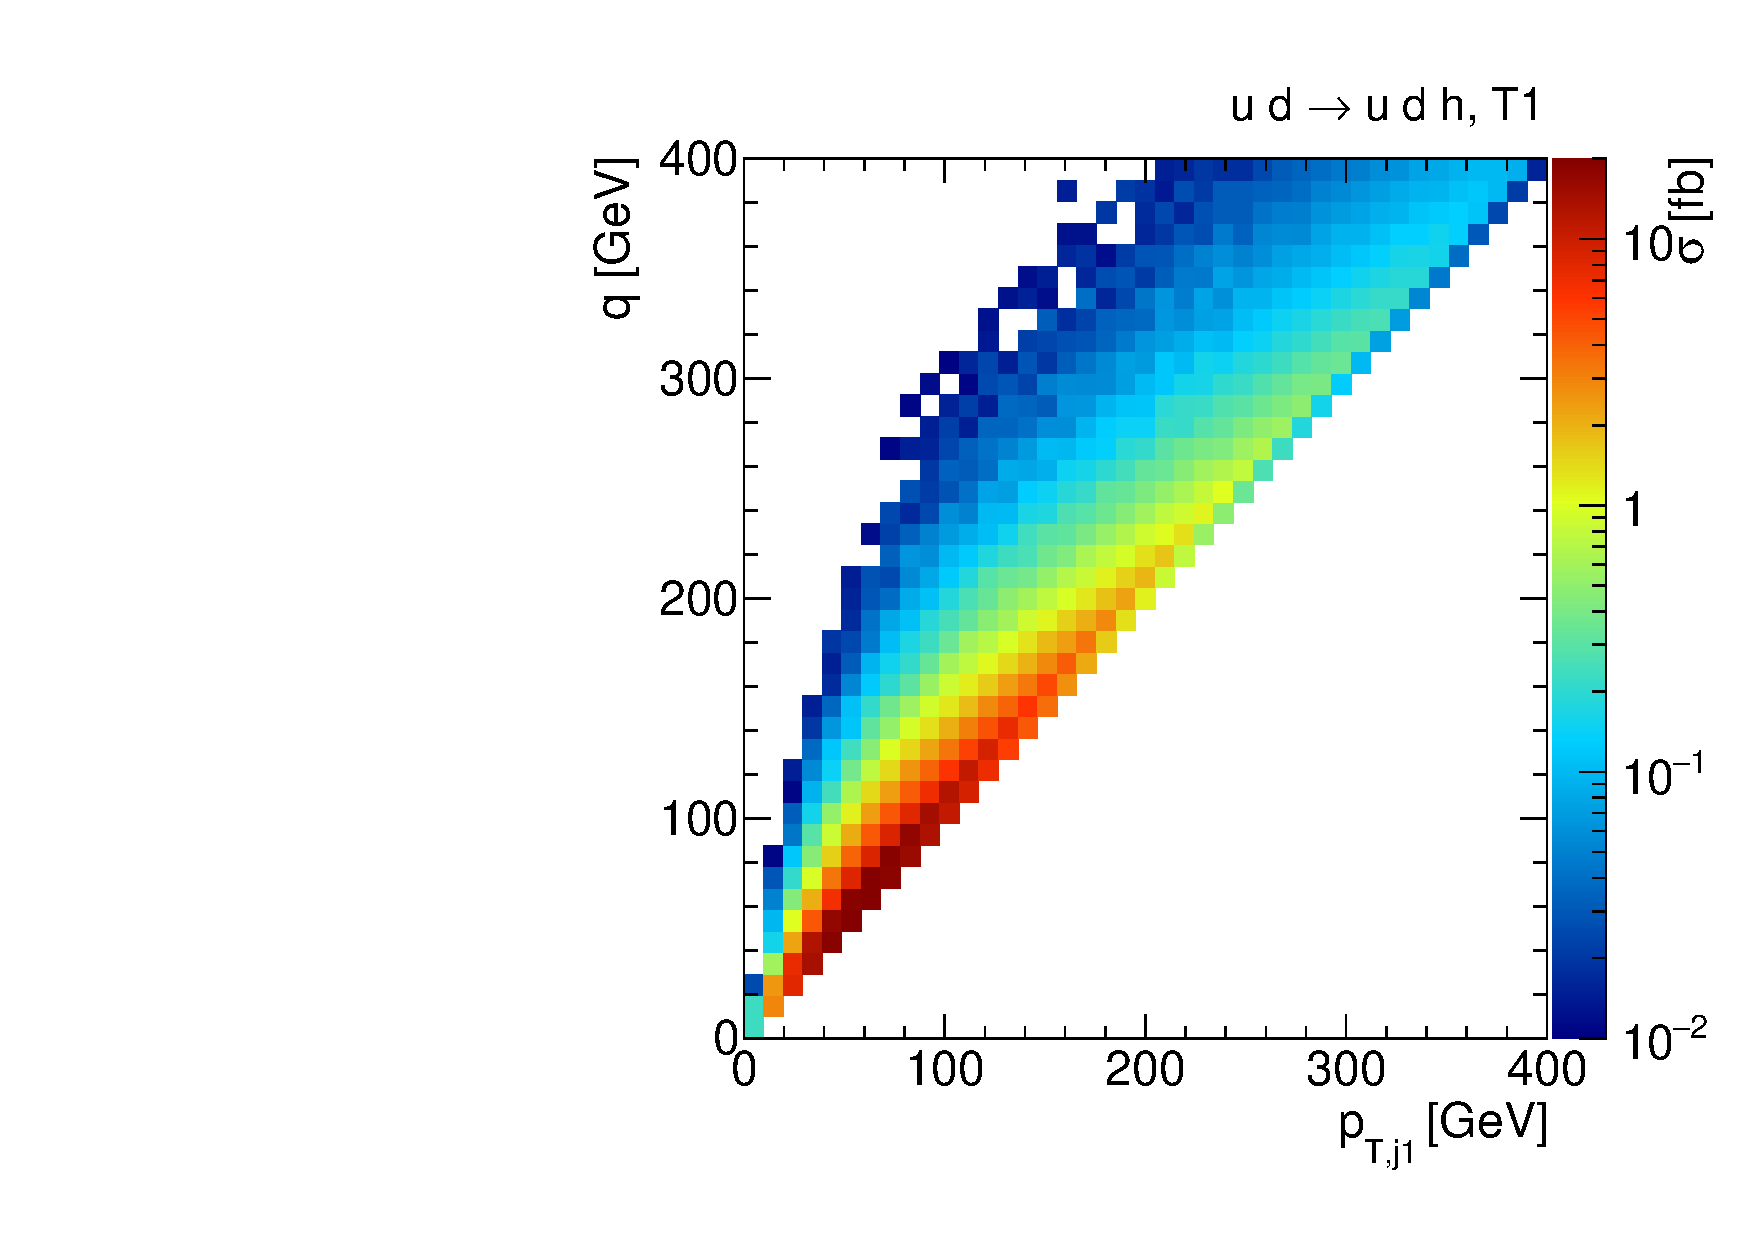
\includegraphics[width=0.49\textwidth]{fig/validity/WBF_correl_q_j1pt.pdf}%
  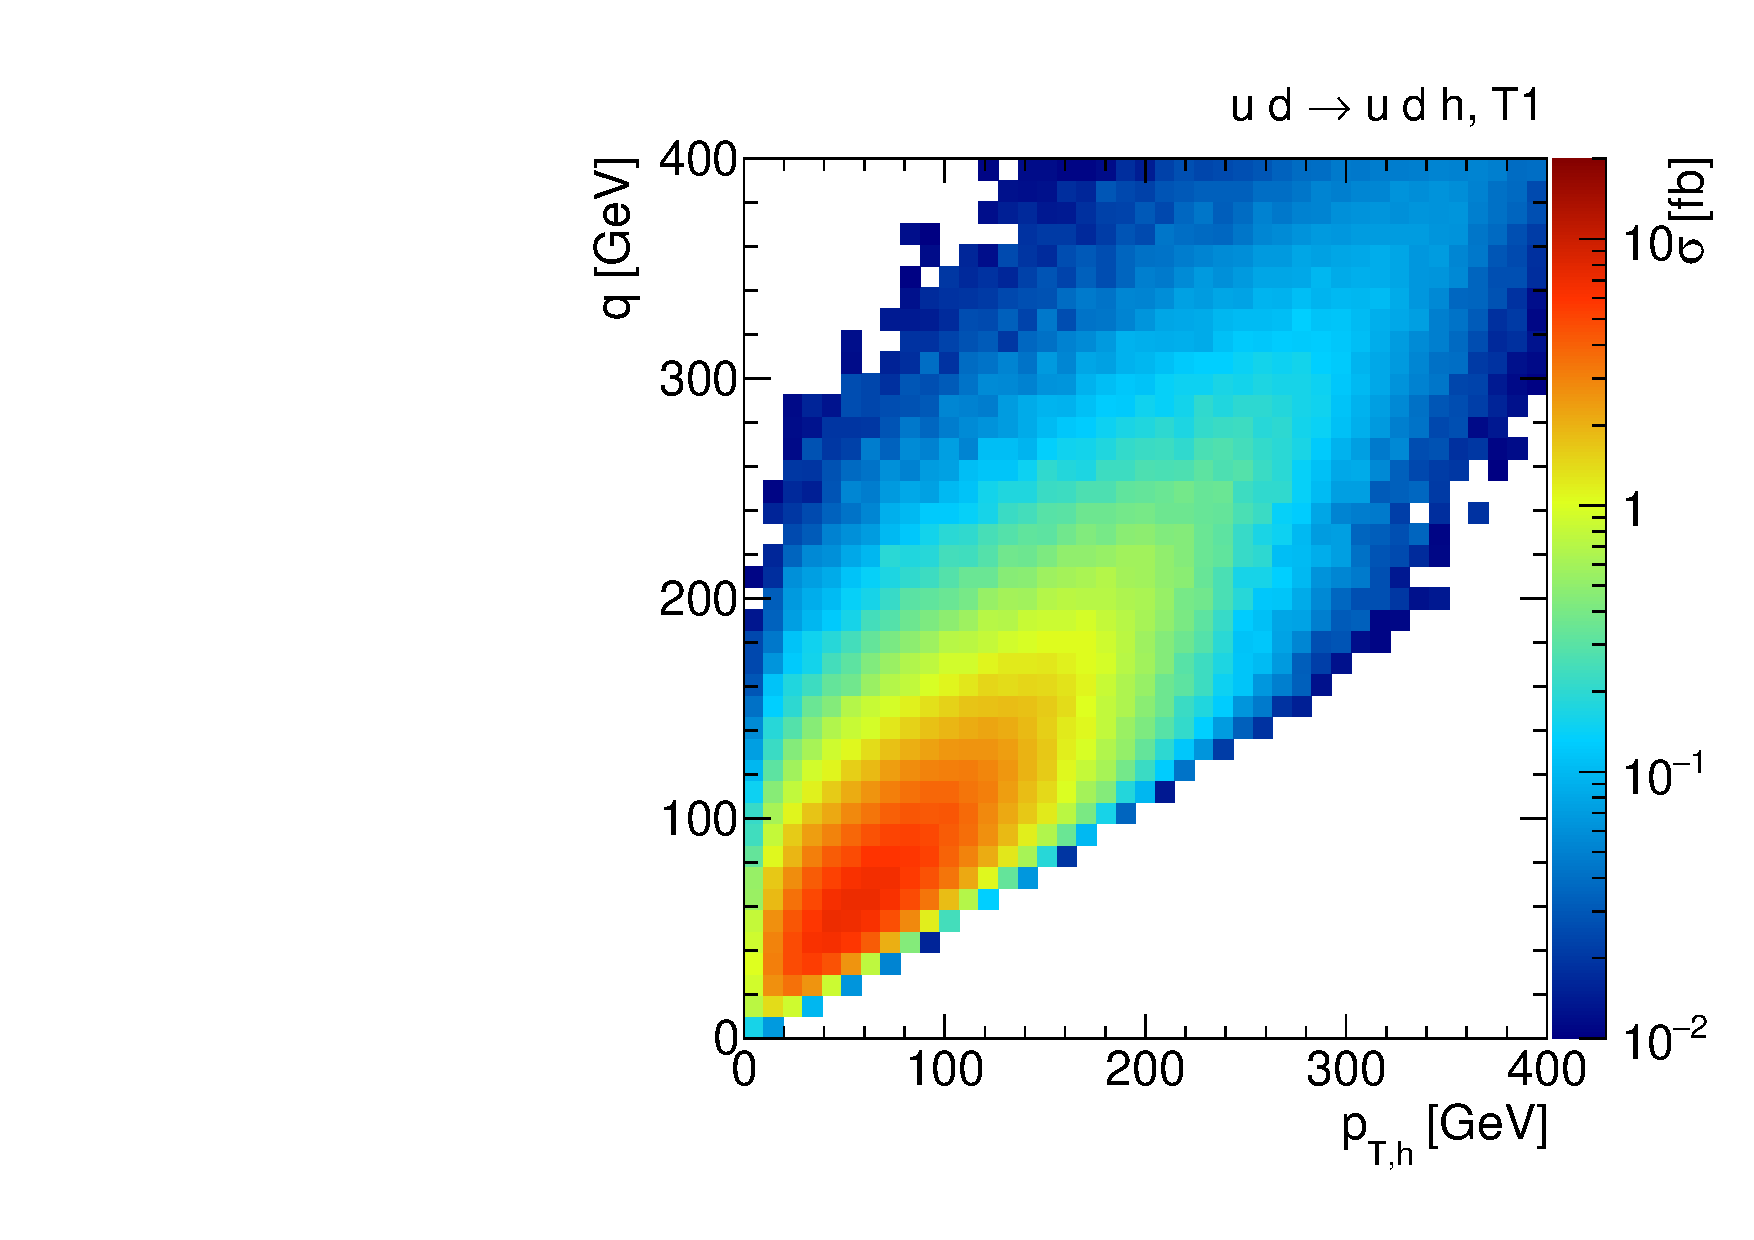
\includegraphics[width=0.49\textwidth]{fig/validity/WBF_correl_q_Hpt.pdf}%
  \caption{Correlations between the WBF momentum transfer $q$, defined
    in \autoref{eq:validity_wbf_virtuality}, and the observable
    transverse momenta $p_{T,j_1}$ (left) and $p_{T,h}$ (right).}
  \label{fig:validity_virtuality_correlations}
\end{figure}

Figure~\ref{fig:validity_virtuality_correlations} shows the
correlations of the transverse momenta of the leading tagging jet or
the Higgs boson with the virtuality $q$. Both are visibly correlated
with the momentum transfer, but the correspondence is particularly
clear for the jet $p_T$.

\newparagraph
%
From the previous section we know that an EFT analysis of kinematic
distributions faces a trade-off: on the one hand, new physics
signatures often grow with the energy scale. On the other hand, the
EFT validity is on a more secure footing at lower energy
scales. However, we have never defined the ``energy scale'' in these
statements quantitatively. We now discuss this choice for WBF Higgs
production. More precisely, we ask which observable $x$ is suitable to
%
\begin{enumerate}
\item isolate phase-space regions with interesting NP signatures with
  a cut $x > x_{\text{min}}$, and simultaneously
\item ensure the EFT validity with a cut $x < x_{\text{max}}$.
\end{enumerate}
%
We compare the observables
%
\begin{equation}
  x \in \left\{  q, \, p_{T,j_1}, \, p_{T,j_2}, \, p_{T,h} \right\} \,.
\end{equation}
%
As discussed above, they all provide probes of the momentum transfer
through the intermediate vector bosons. 

\begin{figure}
  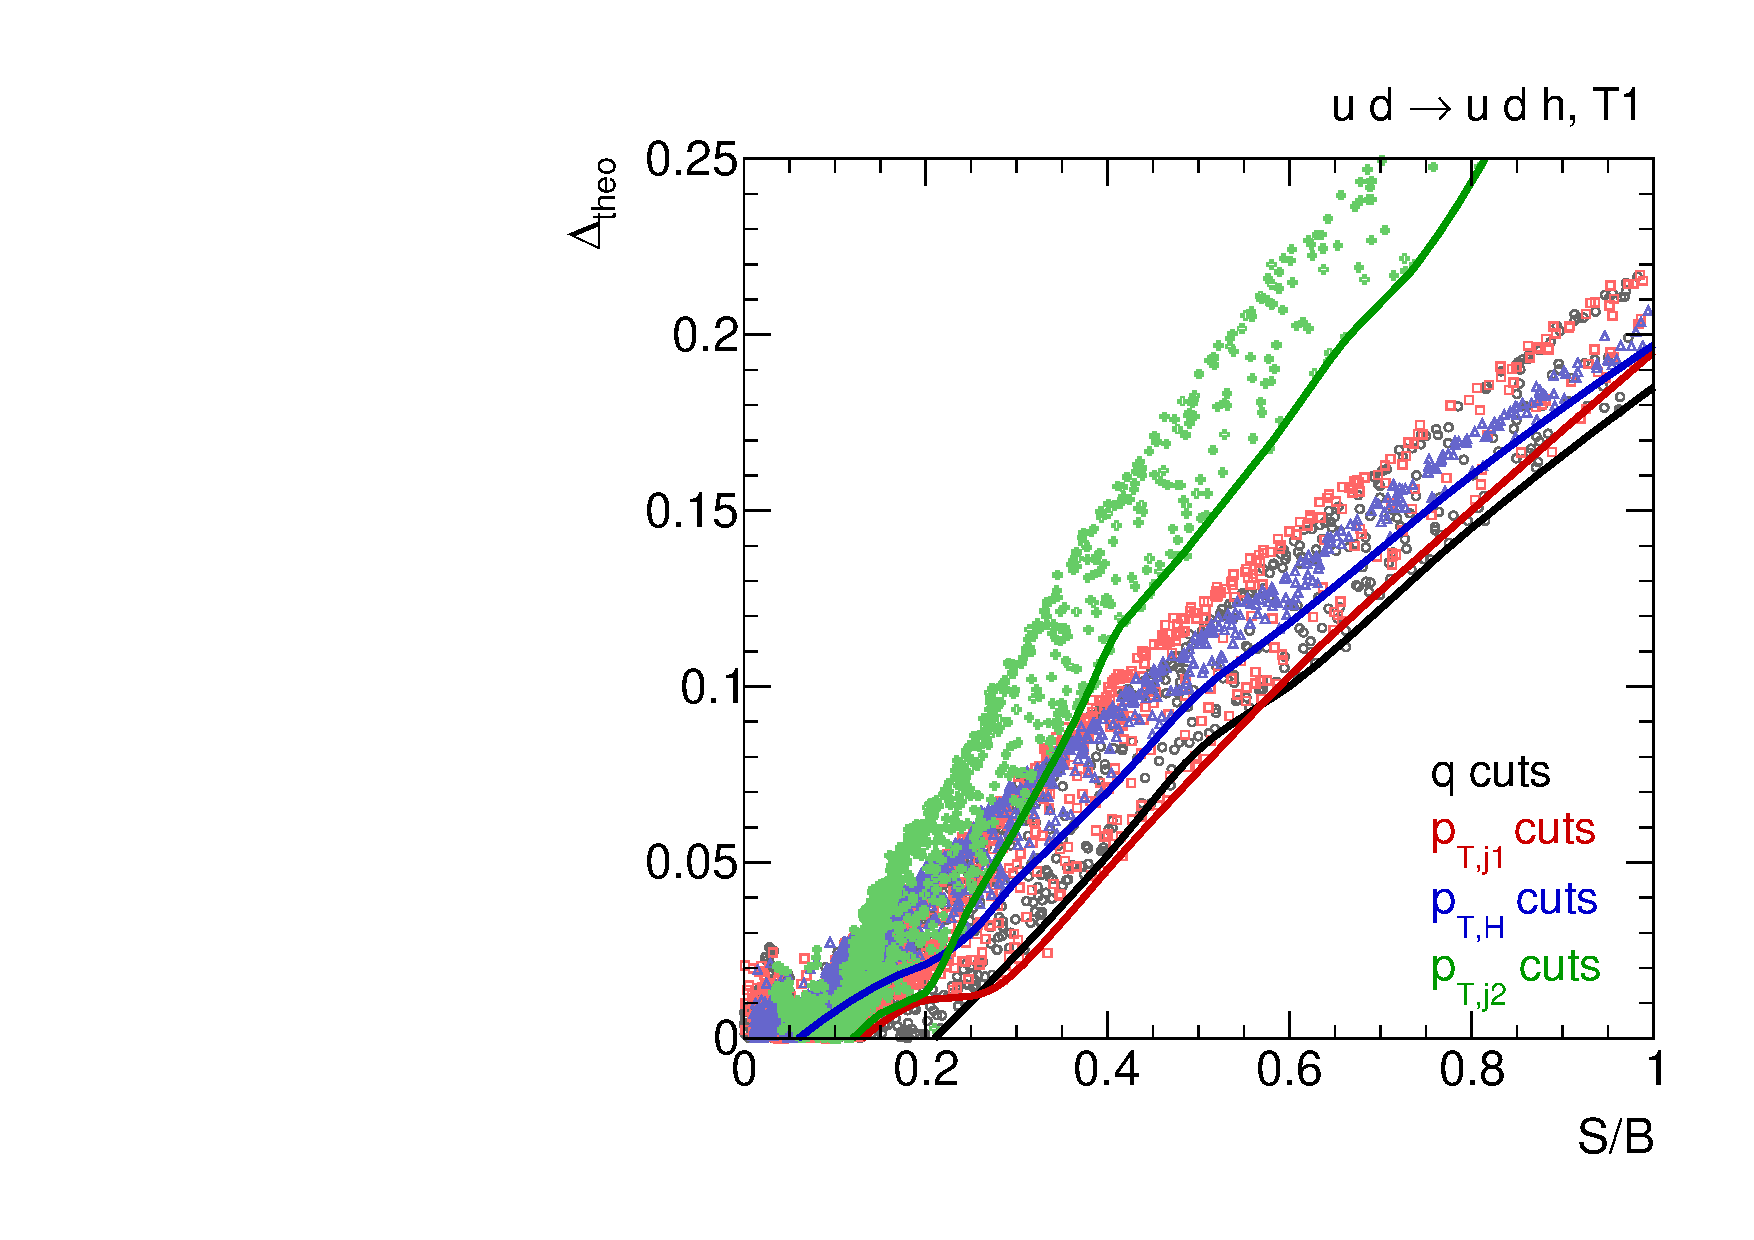
\includegraphics[width=0.49\textwidth]{fig/validity/WBF_cuts_T1_SB.pdf}%
  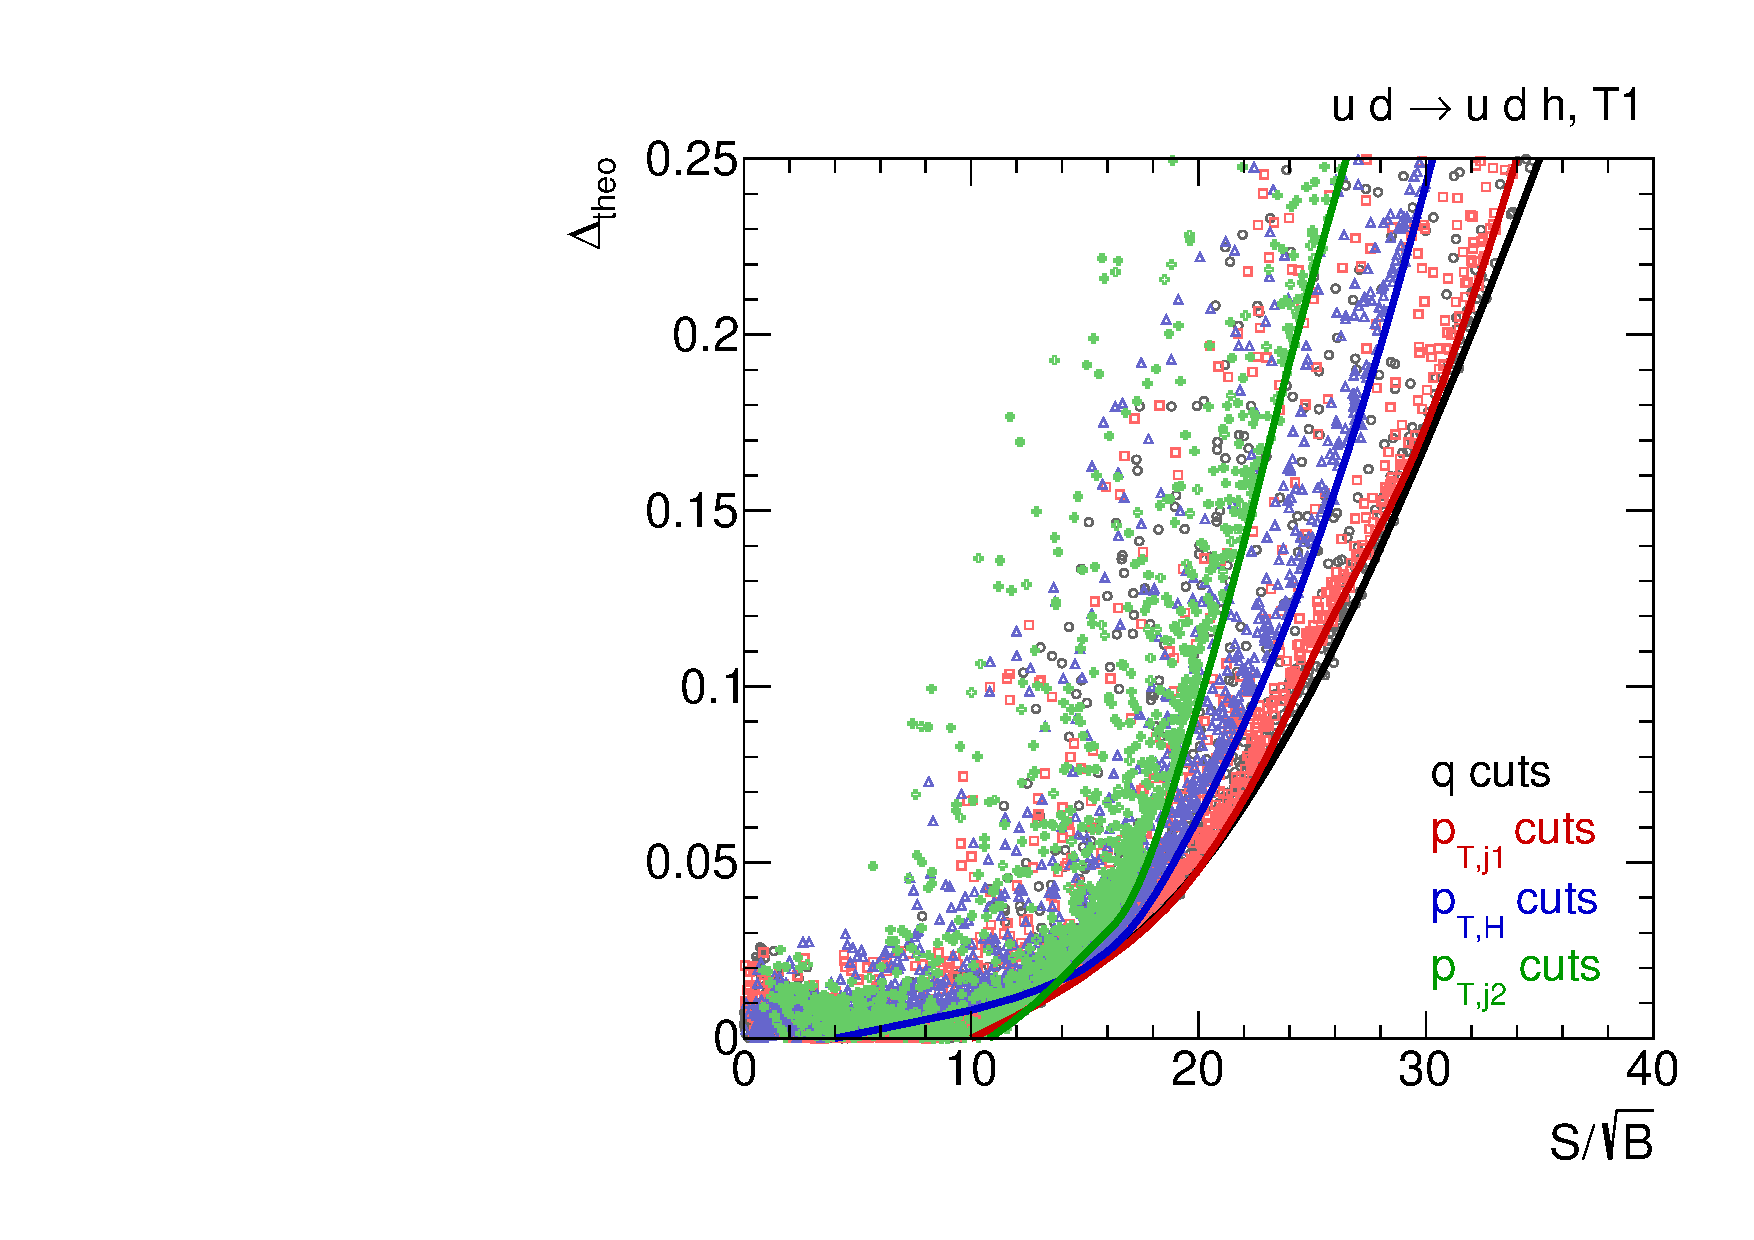
\includegraphics[width=0.49\textwidth]{fig/validity/WBF_cuts_T1_SsqrtB.pdf}%
  \caption{Significance of expected vector triplet signals vs.\
    theoretical uncertainties dimension-six description. Each point
    corresponds to a selection window
    $x_\text{min} < x < x_\text{max}$ in one of the four momentum
    observables
    $x \in \{ q, \, p_{T,j_1}, \, p_{T,j_2}, \, p_{T,h} \}$. See text
    for more details.}
  \label{fig:validity_cuts}
\end{figure}

For each observable $x$ we scan over values of $x_{\text{min}}$ and
$x_{\text{max}}$. For each window $(x_{\text{min}}, x_{\text{max}})$
we calculate the predictions for the parton-level WBF process defined
in \autoref{eq:validity_wbf_proc} for the SM, the vector triplet benchmark
point T1, and the corresponding $v$-improved EFT description. We
reject windows that only leave a signal cross section of less than
20~fb before Higgs decays. We then estimate the significance of the
vector triplet signal over the SM background, disregarding non-Higgs
backgrounds or detector effects for our toy study. In a measurement
limited by systematic uncertainties, the relevant quantity is
%
\begin{equation}
  \frac{S}{B} (x_\text{min}, x_\text{max}) 
= \left| \frac {\sigma_\text{vector triplet} - \sigma_\text{SM}} {\sigma_\text{SM}} \right| \,,
\end{equation}
%
while for a statistics-limited analysis we have to consider
%
\begin{equation}
  \frac{S}{\sqrt{B}} (x_\text{min}, x_\text{max}) 
= \sqrt{L} \, \left| \frac {\sigma_\text{vector triplet} - \sigma_\text{SM}} {\sqrt{\sigma_\text{SM}}} \right| \,.
\end{equation}
%
For our simple illustration we pick an integrated luminosity times
Higgs branching ratio times efficiencies of
$L \times \BR \times \varepsilon = 30~\ifb$.  For each window
$(x_{\text{min}}, x_{\text{max}})$ we also calculate the theory
uncertainty that quantifies the EFT error in this kinematic region as
%
\begin{align}
  \Delta_\text{theo} (x_\text{min}, x_\text{max}) 
  = \left| \frac {\sigma_\text{EFT} - \sigma_\text{vector triplet}} {\sigma_\text{vector triplet}} \right| \,.
\end{align} 

The question is for which observable $x$ we expect significant new
physics signatures, \ie large values of $S/B$ and $S/\sqrt{B}$, while
keeping the EFT error $\Delta_\text{theo}$ small. We show the results
of our scan in Figure~\ref{fig:validity_cuts}. The momentum transfer
$q$ as well as the leading tagging jet's $p_{T,j_1}$ define kinematic
regions with the highest significance for a given theoretical
uncertainty $\Delta_\text{theo}$. This indicates that as long as $q$
is not directly accessible, the transverse momentum of the leading
tagging jet indeed provides the best probe of the momentum flow
through the WBF process, and justifies our choice of observables in
the previous section.



%%%%%%%%%%%%%%%%%%%%%%%%%%%%%%%%%%%%%%%%%%%%%%%%%%%%%%%%%%%%
\subsection{To square or not to square}
\label{sec:validity_squares}
%%%%%%%%%%%%%%%%%%%%%%%%%%%%%%%%%%%%%%%%%%%%%%%%%%%%%%%%%%%%

Differential cross sections are proportional to the squared matrix
element. In our EFT approach, we have
%
\begin{equation}
  |\mat{EFT}|^2
  =
  \underbrace{ |\mat{$4$}^{\vphantom{*}} |^2 }_{\ord{1}}
  + \underbrace{
    2 \, \Real \mat{$4$}^* \mat{$6$}^{\vphantom{*}}
  }_{\ord{1/\Lambda^2}}
  + \underbrace{
    |\mat{$6$}^{\vphantom{*}}|^2 + 2 \, \Real \mat{$4$}^* \mat{$8$}^{\vphantom{*}}
}_{\ord{1/\Lambda^4}}
+ \ord{1/\Lambda^6} \,,
\end{equation}
%
where the subscripts in $\mat{$d$}$ denote the dimension of the
operators in the amplitude, \ie $\mat{$4$}$ is the SM amplitude and
$\mat{$6$}$ contains one dimension-six interaction.  The squared
amplitudes from dimension-six operators contribute at the same order
in the EFT expansion in $1/\Lambda$ as the leading contributions from
dimension-eight operators. This raises the question whether these
squared terms should be included in calculations when dimension-eight
operators are ignored~\cite{Berthier:2015oma, Berthier:2015gja,
  Englert:2015hrx, Greljo:2015sla, Contino:2016jqw, Bylund:2016phk,
  Maltoni:2016yxb}.

In a top-down perspective, \ie knowing the underlying physics, the
answer depends on the typical coupling strengths of the underlying
physics. At least for tree-level effects, the Wilson coefficients of
both dimension-six and dimension-eight operators will generally
contain two couplings of the heavy field, $f_i \sim g_{\text{UV}}^2$, and we
have to compare the terms
%
\begin{equation}
  |\mat{$6$}|^2 \sim \frac {g_{\text{UV}}^4} {\Lambda^4}
  %
  \quad \text{vs.} \quad
  %
  2 \, \text{Re} \mat{$4$}^* \mat{$8$}^{\vphantom{*}} \sim \frac {g_{\text{SM}}^2 g_{\text{UV}}^2} {\Lambda^4} \,,
  \label{eq:validity_square_uv}
\end{equation}
%
where $g_{\text{SM}}$ denotes a typical SM coupling. In strongly coupled
scenarios we therefore expect the squared dimension-six terms to
dominate over the dimension-eight contributions, and it is perfectly
justified to include the squared dimension-six term, but no
dimension-eight operators. In more weakly coupled models with
$g_{\text{UV}} \sim g_{\text{SM}}$, the two should approximately contribute equally.
The size of the squared dimension-six terms can then be seen as an
estimate for the size of the missing higher orders in the EFT
expansion, and therefore as an indicator for the validity of the EFT
approach~\cite{Englert:2015hrx}.

Of course, in practice we do not know the coupling strength of UV
physics. Generally discarding the squared dimension-six terms will
degrade the EFT performance at least for strongly coupled
scenarios. Similarly, universally using the size of the squared
dimension-six amplitude as a theory error in global fits introduces a
theory dependence in the results.

Note also that the argument in \autoref{eq:validity_square_uv} relies
on the assumption that except for the typical couplings and the
suppression scale $\Lambda$ all amplitudes have approximately the same
size. But in phase-space regions where the dimension-four contribution
is suppressed, the dimension-six squared term can easily be larger
than the interference between the SM and the dimension-eight amplitude, even if
the EFT expansion in $v/\Lambda$ holds and higher-dimensional
operators are negligible. One example is Higgs pair production with
its accidental cancellation between the two SM contributions, as
discussed in \autoref{sec:foundations_channels} and demonstrated in
\ref{sec:validity_singlet}.

\begin{figure}
  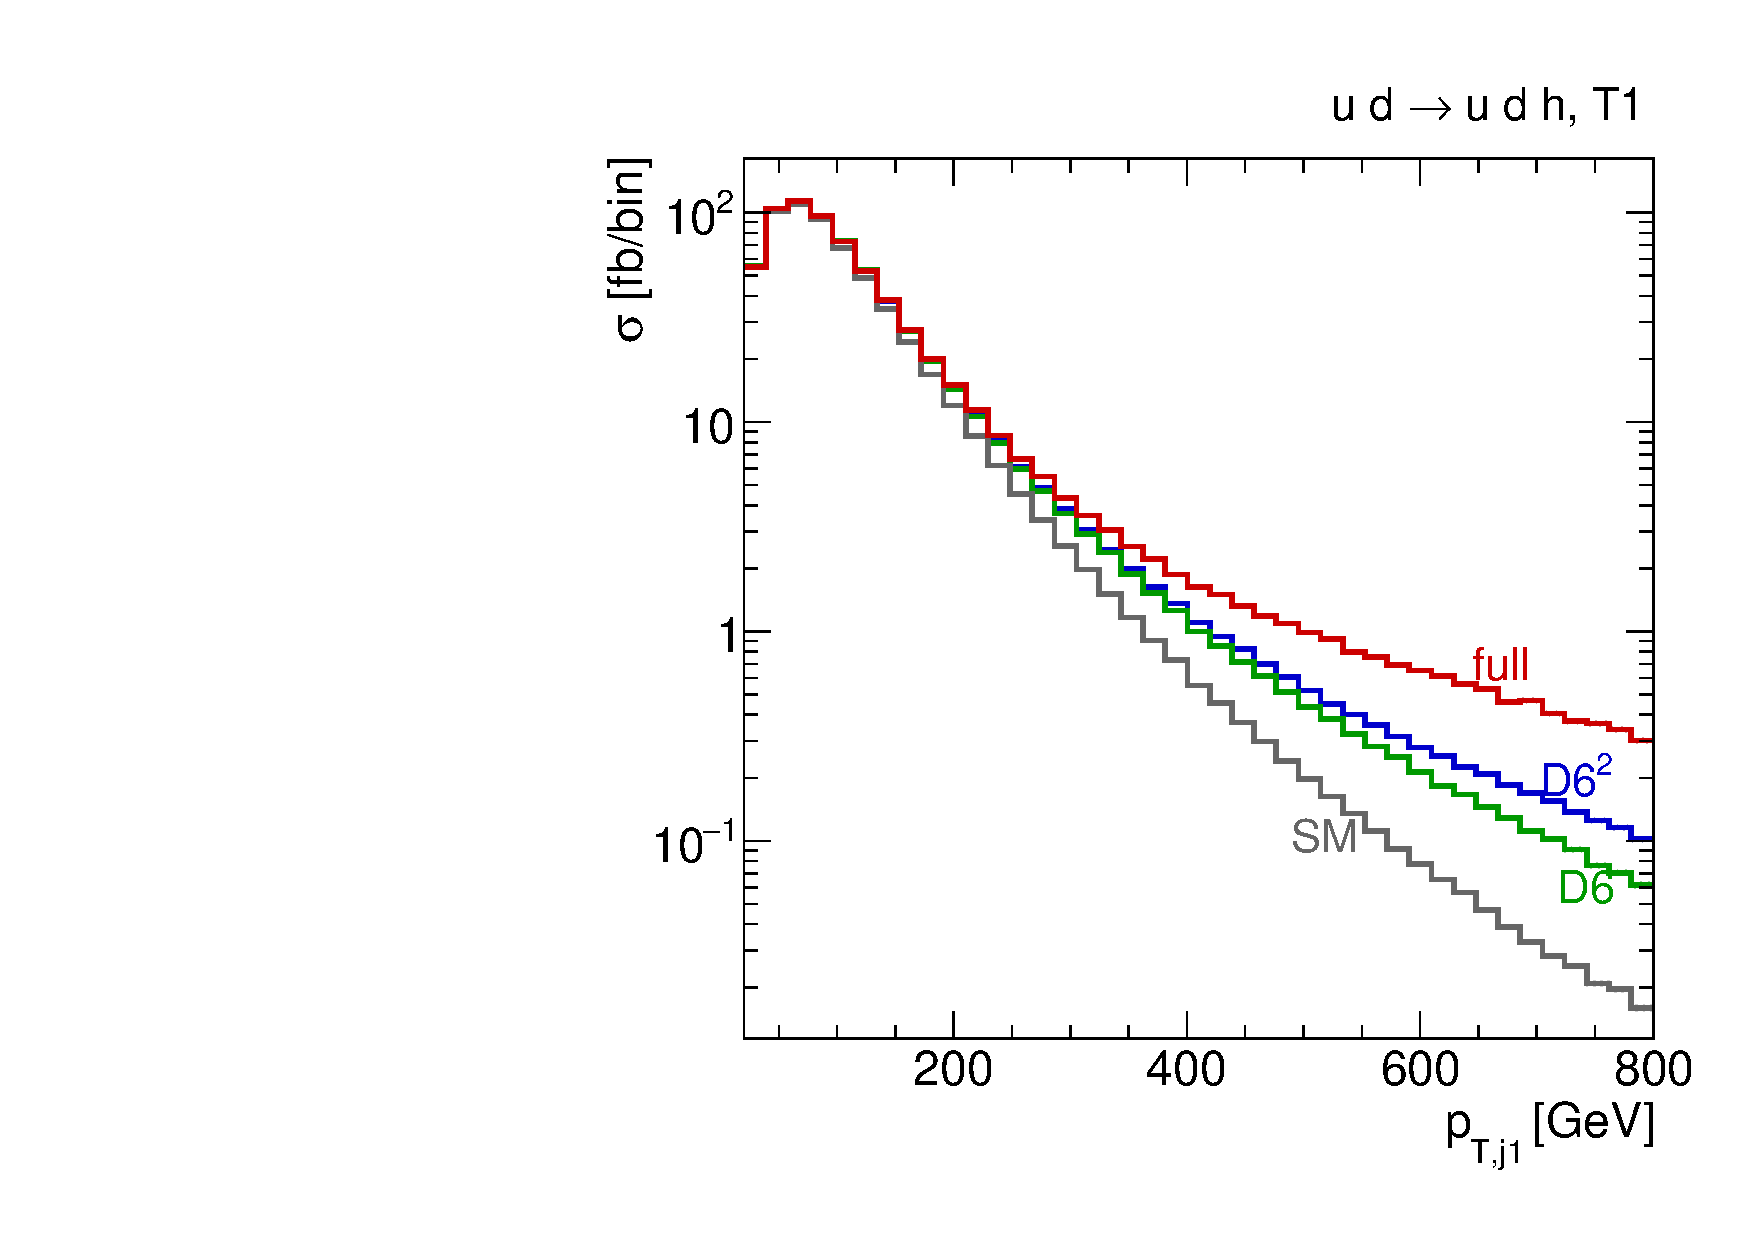
\includegraphics[width=0.49\textwidth]{fig/validity/WBF_T1_j1pt.pdf}%
  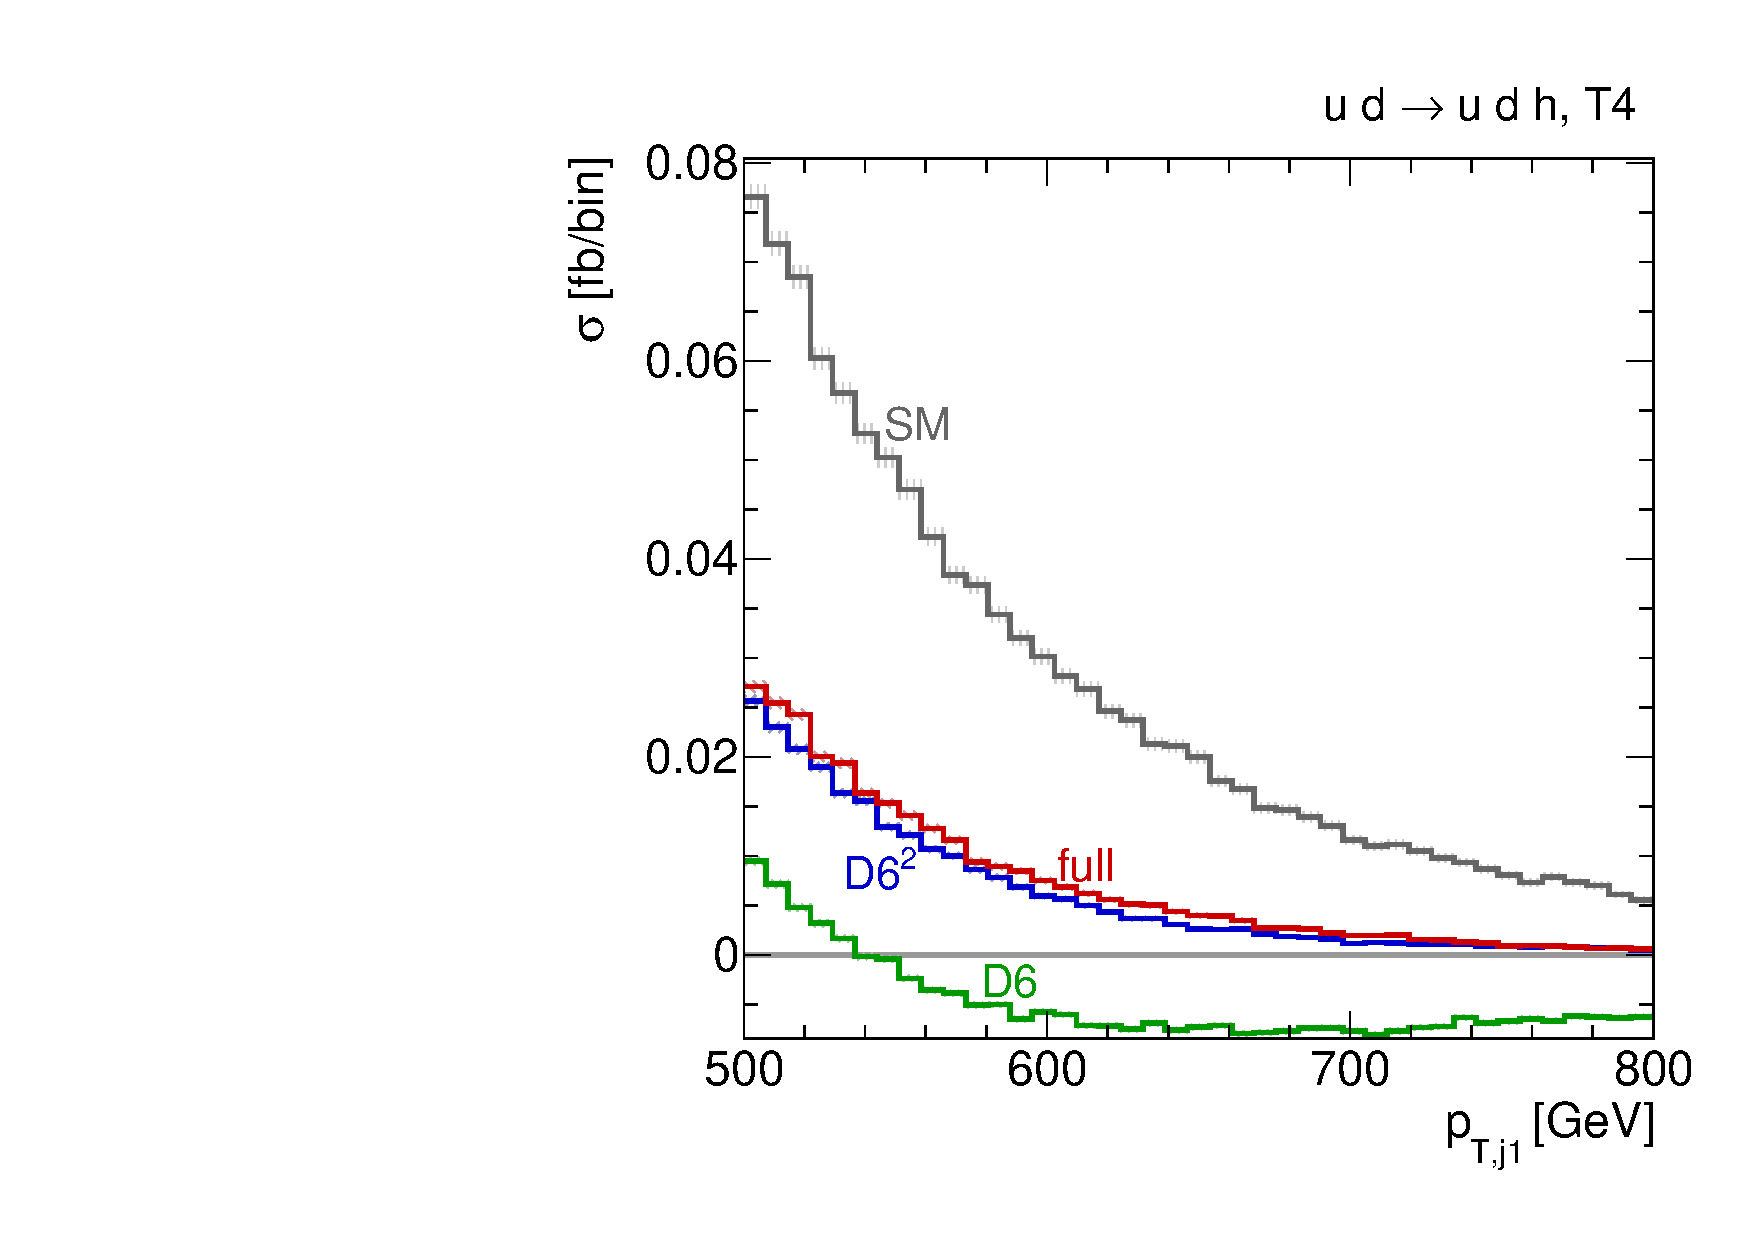
\includegraphics[width=0.49\textwidth]{fig/validity/WBF_T4_j1pt_zoom.pdf}%
  \caption{WBF distributions with (``D6$^{2}$'') and without (``D6'')
    the squared amplitudes from dimension-six operators. The right
    panel zooms in on the region where leaving out the squared
    dimension-six terms leads to a negative cross section.}
  \label{fig:validity_squared}
\end{figure}

If we consider the dimension-six Lagrangian not as the leading term of
a consistent effective field theory, but rather as a phenomenological
parametrisation describing a vast range of LHC Higgs signatures, the
counting argument becomes irrelevant and the square of dimension-six
terms should always be included.

Finally, from a technical perspective the squared dimension-six terms
are necessary to guarantee positive cross sections. Without them, the
expected rate can become negative in high-energy tails or in other
regions of the phase space where the SM predictions are small. 

\autoref{fig:validity_squared} demonstrates these considerations,
again with WBF Higgs production in the vector triplet model. The
squared dimension-six terms improve the agreement with the full model,
and in one of the two benchmarks shown they are also necessary to
avoid negative rates in the high-energy tail of the distribution.

To conclude, a simple expansion in $1/\Lambda$ suggests that the
square of dimension-six amplitudes should not be taken into account in
calculations within the dimension-six framework. But this argument is
only valid if the underlying physics is weakly coupled and in
phase-space regions with sizeable contributions from the SM. In these
situations no harm is done by including the squared dimension-six
terms. Since their inclusion can improve the EFT validity in many
other scenarios and is necessary to guarantee positive cross sections,
we recommend to include these terms in most situations.



%%%%%%%%%%%%%%%%%%%%%%%%%%%%%%%%%%%%%%%%%%%%%%%%%%%%%%%%%%%%
\subsection{Limit setting}
\label{sec:validity_fits}
%%%%%%%%%%%%%%%%%%%%%%%%%%%%%%%%%%%%%%%%%%%%%%%%%%%%%%%%%%%%

An important purpose of the dimension-six Lagrangian is to act as an
intermediate parametrisation in the process of using Higgs
measurements to set exclusion limits on the parameter space of
specific models. We now test explicitly if limits derived in this way agree
with constraints directly calculated in the full model.

We follow a simplified limit setting procedure. Expected exclusion
limits on the vector triplet in the absence of a signal are
calculated, either directly based on the full model, or first on the
dimension-six Wilson coefficients and then translated onto the full
model. Motivated by the discussion in the previous section, we also
calculate limits on the dimension-six Wilson coefficients without
taking into account the squared dimension-six contributions, and again
translate the results to the vector triplet parameters. As a process
we consider WBF Higgs production as given in
\autoref{eq:validity_wbf_proc} and multiply the total Higgs production
cross sections with a branching ratio
$\BR(h \to 2\ell 2\nu) \approx 0.01$.  We disregard non-Higgs
backgrounds as well as parton-shower or detector effects. Our limits
are based on expected event counts in two high-energy bins of the
$p_{T,j_1}$ distributions. We define a parameter point to be excluded
if $S/\sqrt{S+B} > 2$. While this statistical analysis is not designed
to be realistic, it illustrates how the validity of our dimension-six
approach affects possible limits.

We consider a two-dimensional plane in the parameter space of the
vector triplet model. It is spanned by the mass $m_\xi$ and a
universal coupling rescaling $c$, and we choose the couplings as
%
\begin{equation}
  g_V = 1 \,, \qqquad 
  c_H = c \,, \qqquad 
  c_F = \frac {g_V^2}{2g^2} \, c \,, \qqquad 
  c_{HHVV} = c^2
\end{equation}
%
such that the Wilson coefficients $f_{\phi,2}$, $f_{\phi,3}$, and $f_{t}$ vanish,
%
\begin{equation}
  f_{WW} = f_{BW} = \frac {c^2} {2g^2} \,,
\end{equation}
%
and
%
\begin{equation}
  f_W = - \frac {c^2} {g^2} \,.
\end{equation}
%
In this parameter plane, all amplitudes from dimension-six operators
scale with $c^2/m_\xi^2$. Our perturbative calculation does makes
sense for very strongly interacting systems, so we limit our analysis
to $\Gamma_{\xi}/m_{\xi} < 1/4$.

\begin{figure}
  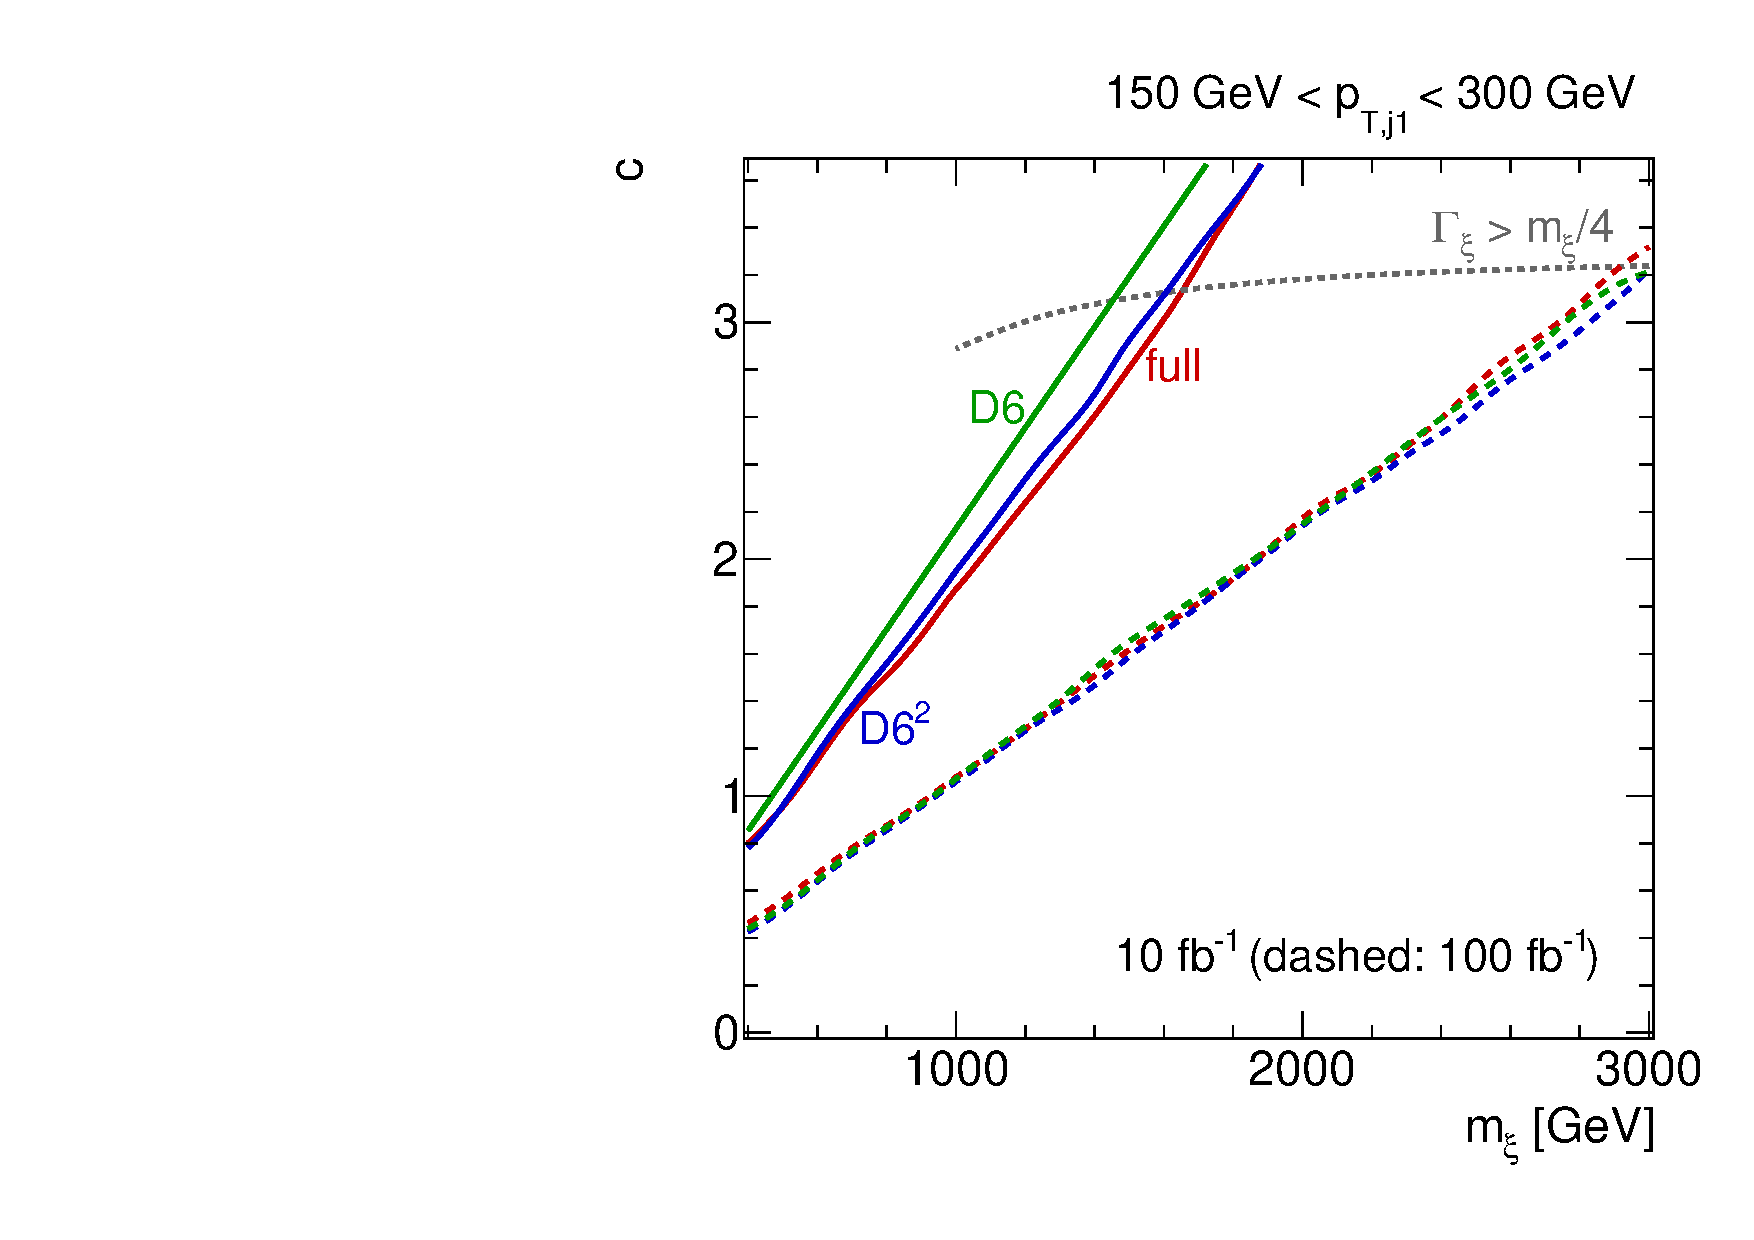
\includegraphics[width=0.49\textwidth]{fig/validity/WBF_limits_150.pdf}%
  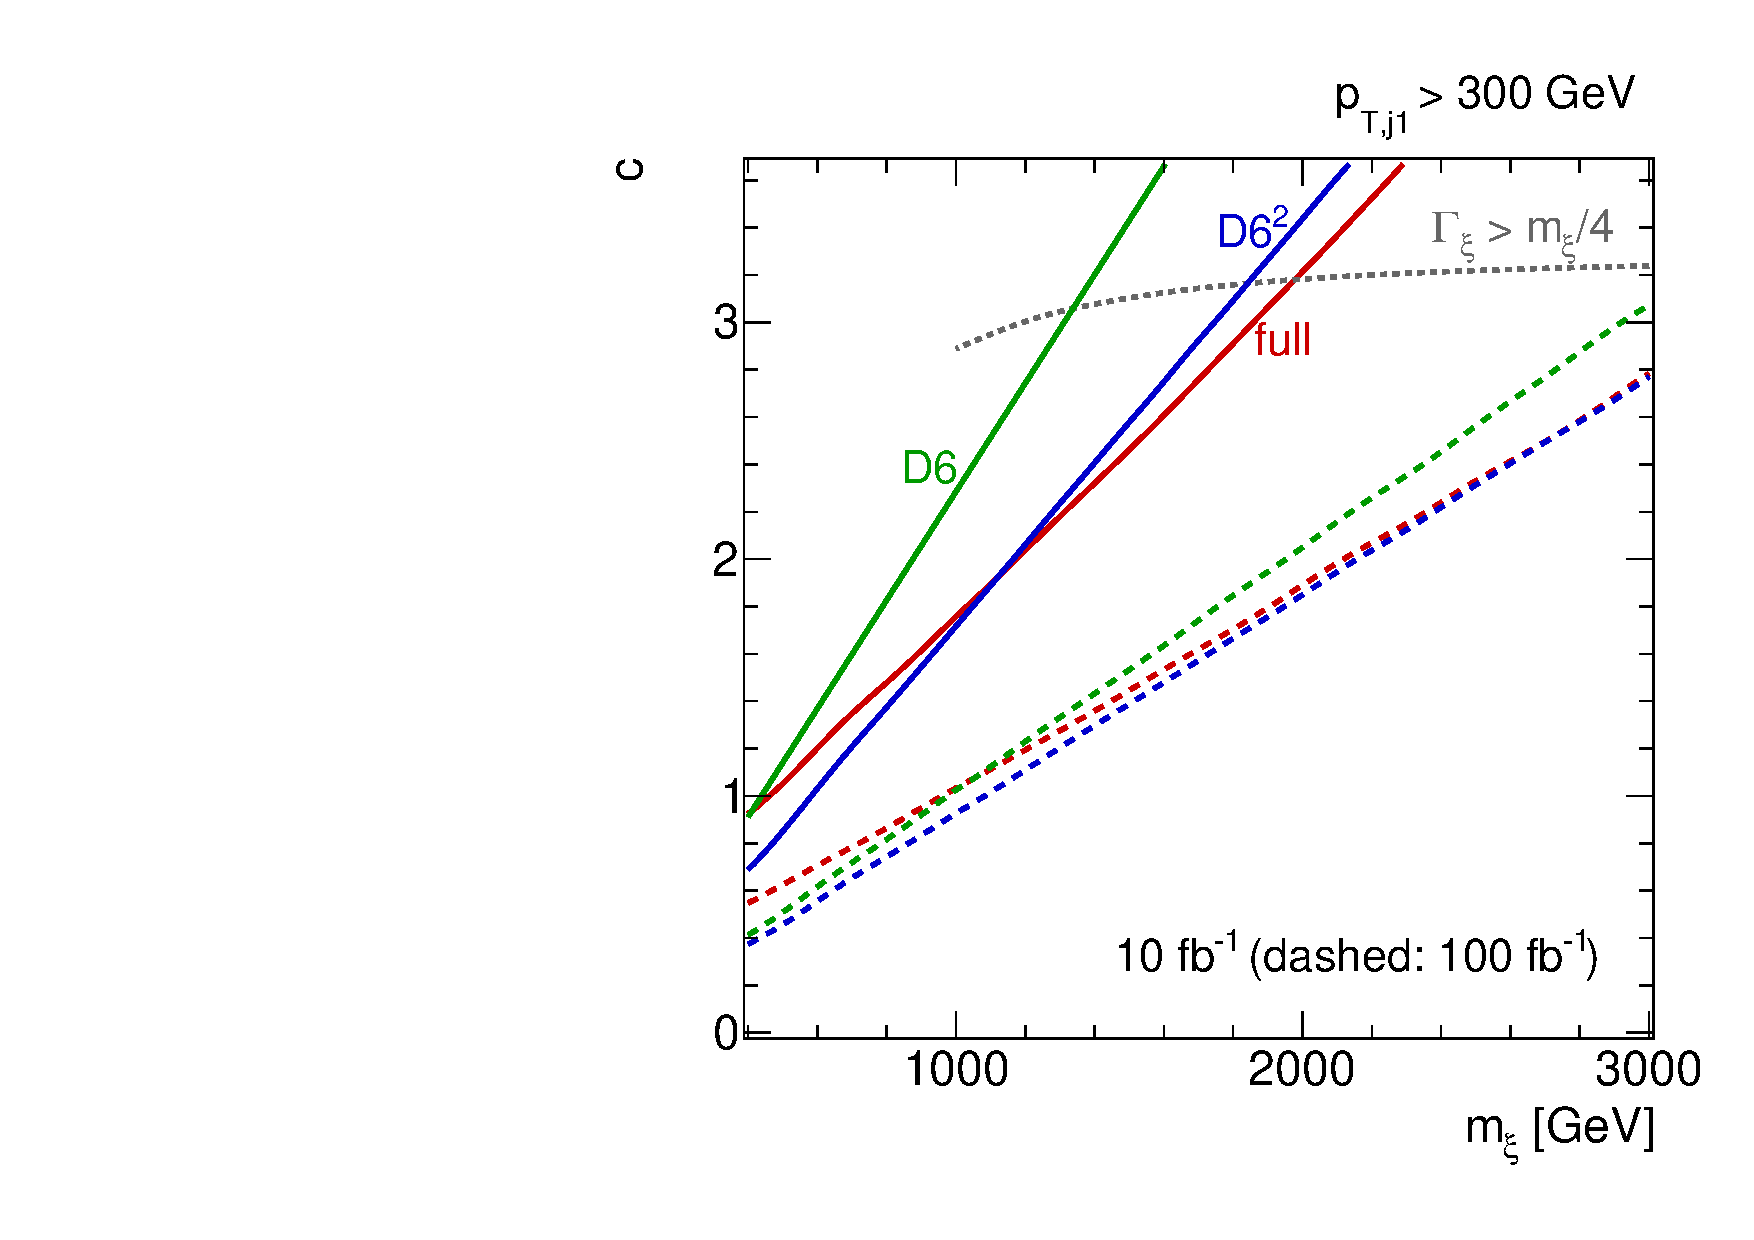
\includegraphics[width=0.49\textwidth]{fig/validity/WBF_limits_300.pdf}%
  \caption{Toy limits on a two-dimensional slice of the vector triplet
    parameter space. We show the analysis based on the event numbers
    in $150~\gev < p_{T,j_1} < 300~\gev$ (left) and based on the tail
    $p_{T,j_1} > 300$~GeV (right).}
  \label{fig:validity_limits}
\end{figure}

The resulting toy limits are shown in
\autoref{fig:validity_limits}. Based on event numbers in the range
$150~\gev < p_{T,j_1} < 300~\gev$, constraints calculated directly in
the full model and EFT limits translated to the vector triplet agree
very well. The inclusion of the dimension-six squared terms, however, can be
important for this agreement. With more statistics, the differences
between the various procedures become smaller, and ultimately the
question of whether the squared dimension-six amplitudes should be
taken into account is rendered irrelevant.

Larger differences appear when we use the information from the
high-energy tail $p_{T,j_1} > 300$~GeV to constrain vector bosons with
masses down to $m_\xi \gtrsim 500~\gev$. This lack of a scale
hierarchy does not improve with more statistics. The high-energy tail
is also more sensitive to the square of dimension-six terms.



%%%%%%%%%%%%%%%%%%%%%%%%%%%%%%%%%%%%%%%%%%%%%%%%%%%%%%%%%%%%
\section{Conclusions}
\label{sec:validity_conclusions}
%%%%%%%%%%%%%%%%%%%%%%%%%%%%%%%%%%%%%%%%%%%%%%%%%%%%%%%%%%%%

The dimension-six operators of linear Higgs effective field theory
provide a theoretically well-defined, largely model-independent, and
phenomenologically powerful framework to parametrise deviations from
the Standard Model. But the validity of the EFT approach relies on a
gap between the experimental momentum transfer and the mass scales of
the probed models of new physics. The limited precision of the LHC can
guarantee such a clear scale hierarchy only under the additional
assumption that the underlying physics is strongly coupled. For
moderately weakly to moderately strongly coupled models, LHC Higgs
measurements are sensitive to new physics scales ranging from the
electroweak scale to approximately one TeV, casting doubt on the
validity of the EFT approximation.

In this chapter we have studied the usefulness of the effective theory
for LHC Higgs measurements by comparing different complete models of
new physics to their descriptions in terms of dimension-six
operators. Our comparison included a singlet extension of the Higgs
sector, a two-Higgs doublet model, scalar top partners, and a heavy
vector triplet, focusing on parameter ranges relevant for the LHC. We
analysed Higgs couplings, total production rates, and kinematic
distributions for the main Higgs production modes and representative
decay channels.

A naive construction of the dimension-six model, where the effective
theory is matched to the full model in the unbroken phase of the
electroweak symmetry, confirms the concerns based on an estimate of
the energy scales: such a dimension-six approximation does not
describe the phenomenology of many models adequately. In Higgs
couplings and total production rates, the discrepancies between the
full model and its effective counterpart are of the order of
$v^2 / \Lambda^2$, where $\Lambda$ is the new physics scale. In the
high-energy tails of distributions, the EFT error even scales with
$E^2 / \Lambda^2$. For many weakly coupled scenarios relevant for LHC
Higgs measurements, this implies an unacceptably large error.

But this is not the end of the story. As we discussed at length in
\autoref{sec:validity_matching}, matching the dimension-six model to
the full theory is not unambiguous. First, instead of setting the
matching scale $\Lambda$ to the intrinsic new physics scale in the
Lagrangian, we can use the actual physical masses after electroweak
symmetry breaking, including contributions from the electroweak
VEV. Second, we can express the Wilson coefficients of the
dimension-six operators in terms of physical quantities such as mixing
angles instead of Lagrangian parameters. These alternative choices,
which we collectively call ``$v$-improved matching'', amount to
matching the EFT in the broken phase of the electroweak symmetry.

While a $v$-improved EFT construction may be unconventional from a
purely theoretical perspective, expressing quantities in physical
masses and mixing angles is a natural choice from a practical point of
view. It can be interpreted as a partial absorption of the
dimension-eight and higher operators of the form $(\phisq)^n \ope{i}$
into the Wilson coefficients of dimension-six operators with the
replacement $\phisq \to v^2 / 2$. In this way, it can improve the
effective description where the expansion in $v/\Lambda$ converges
slowly for the default matching; it cannot help in high-energy tails
where $E/\Lambda$ becomes large. Note that $v$-improvement does not
change the form of the effective operators, nor does it affect their
phenomenology, or the way that experimental collaborations should set
limits on operators. It purely affects the interpretation of Wilson
coefficients in terms of model parameters.

\begin{table}
\begin{tabular}{ll c ccc}
  \toprule
  %
  Model & Process && \multicolumn{3}{c}{EFT failure} \\
  %
  \cmidrule{4-6}
  %
  & && rates & kinematics & matching \\
  %
  \midrule
  %
  singlet & on-shell $h \to 4 \ell$, WBF, $Vh$ && & & \largex \\
        & off-shell WBF  && & \brlargex & \largex \\
        & $hh$ && \largex & \largex & \largex \\
  %
  2HDM & on-shell $h \to 4 \ell$, WBF, $Vh$ && \brlargex & & \largex \\
        & off-shell $h \to \gamma \gamma$ && & \brlargex & \largex \\
        & $hh$ && \largex & \largex & \largex \\
  %
  top partners & WBF, $Vh$ && \brlargex & & \brlargex \\
  %
  vector triplet & WBF && & \brlargex & \largex \\
        & $Vh$ && & \brlargex & \largex \\
  %
  \bottomrule
\end{tabular}
\caption{Possible sources of failure of the dimension-six Lagrangian in Higgs
  observables. In addition, new light resonances that
  contribute to the same final states present an obvious breakdown of the
  effective description. We use parentheses where deviations appear, but are unlikely to
  be observed in realistic scenarios. }
 \label{tbl:validity_breakdown_summary}
\end{table}

We find that with a $v$-improved matching procedure the dimension-six
operators provide an adequate description in almost all scenarios. The
exceptions that confirm the rule are summarised in
\autoref{tbl:validity_breakdown_summary}. The singlet and doublet
extensions of the Higgs sector lead to simple shifts of the SM Higgs
couplings, effects mostly well captured by the corresponding
dimension-six operators. The effective description struggles with
shifts of the Higgs-gauge couplings in the 2HDM, which only appear at
dimension eight in the EFT. A more dramatic breakdown occurs in Higgs
pair production, where two types of SM diagrams approximately cancel
and off-shell contributions from new resonances have a large impact.
With the scalar top partners, we illustrate that loop effects in
Higgs-gauge couplings are either too small to be relevant for the LHC,
or require light new particles and large couplings, in which case the
effective description clearly breaks down. The vector triplet model
generates interesting kinematic effects in $Vh$ and WBF Higgs
production at tree level. A $v$-improved dimension-six model can
describe these effects over a large part of the phase space for
realistic scenarios, breaking down only in the high-energy tails of
certain kinematic distributions. Finally, the effective theory fails
to describe new light resonances. Such a signature at the LHC would be
an obvious signal to switch to an appropriate simplified model.

Focusing on Higgs production in weak boson fusion in the vector
triplet model, we proceeded with a set of practical questions. First,
we studied how the momentum transfer in weak boson fusion can be
defined and measured, confirming the established notion that the
transverse momenta of the tagging jets provide the most useful probe
of the energy flow. We discussed the role of squared dimension-six
amplitudes, which contribute to cross sections at the same order in
the EFT expansion as the leading effects from the neglected
dimension-eight operators. Nevertheless, these squared terms can
improve the performance of the dimension-six model in many cases and
should in general be included in calculations from a bottom-up
perspective. We concluded our discussion of the vector triplet model
with a brief demonstration of how the validity of the dimension-six
model affects the setting of exclusion limits in practice. The
effective theory is less reliable when very high-energy events are
taken into account. This suggests that experiments should constrain
Wilson coefficients not only with the full event samples, but also
with additional upper bounds on the momentum transfer; alternatively,
momentum-dependent theory uncertainties can be assigned to the
events~\cite{Berthier:2016bke}.

With the limited precision of the LHC, the EFT approach is not
guaranteed to describe all potential signatures of new physics in
Higgs measurements accurately. Nevertheless, we have demonstrated that
the dimension-six model works remarkably well for a wide range of
models, parameter choices, and observables in single Higgs
production. Key to this good performance is a suitable matching
procedure, which takes into account subleading contributions from the
Higgs VEV. This does not present a complication for an experimental
fit of dimension-six operators to LHC Higgs data, it is purely a
theoretical aspect for the interpretation of the results.
